
\documentclass[10.5pt,dutch,]{article}
\usepackage{lmodern}
\usepackage[hyphens]{url}
\makeatletter
\g@addto@macro{\UrlBreaks}{\UrlOrds}
\makeatother
\expandafter\def\expandafter\UrlBreaks\expandafter{\UrlBreaks%  save the current one
  \do\a\do\b\do\c\do\d\do\e\do\f\do\g\do\h\do\i\do\j%
  \do\k\do\l\do\m\do\n\do\o\do\p\do\q\do\r\do\s\do\t%
  \do\u\do\v\do\w\do\x\do\y\do\z\do\A\do\B\do\C\do\D%
  \do\E\do\F\do\G\do\H\do\I\do\J\do\K\do\L\do\M\do\N%
  \do\O\do\P\do\Q\do\R\do\S\do\T\do\U\do\V\do\W\do\X%
  \do\Y\do\Z}

\usepackage{amssymb,amsmath}
\usepackage{ifxetex,ifluatex}
\usepackage{fixltx2e} % provides \textsubscript
\ifnum 0\ifxetex 1\fi\ifluatex 1\fi=0 % if pdftex
  \usepackage[T1]{fontenc}
  \usepackage[utf8]{inputenc}
\else % if luatex or xelatex
  \ifxetex
    \usepackage{mathspec}
  \else
    \usepackage{fontspec}
  \fi
  \defaultfontfeatures{Ligatures=TeX,Scale=MatchLowercase}
    \setmainfont[]{CMU Serif}
    \setsansfont[]{CMU Sans Serif}
    \usepackage{xeCJK}[2012/04/08 v3.0.0]
    \xeCJKDeclareSubCJKBlock{Hangul}{"1100 -> "11FF, "3130 -> "318F, "A960 -> "A97F, "AC00 -> "D7AF, "D7B0 -> "D7FF}
    %\xeCJKDeclareSubCJKBlock{Kana}{"3040 -> "309F, "30A0 -> "30FF, "31F0 -> "31FF, "1B000 -> "1B0FF}
    \setCJKmainfont[]{Kozuka Mincho Pro}
    \setCJKmainfont[Hangul]{Gulim}
%


%\setmainfont{CMU Serif}

%\usepackage{xeCJK}
%\setCJKmainfont{Kozuka Mincho Pro} % for Cn & Jp
%\setCJKmonofont{Gulim} % for Kr

%\usepackage{xeCJK}[2012/04/08 v3.0.0]



%\setCJKmainfont{SimSun}
%\setCJKmainfont[Kana]{Kozuka Mincho Pro}

\fi
% use upquote if available, for straight quotes in verbatim environments
\IfFileExists{upquote.sty}{\usepackage{upquote}}{}
% use microtype if available
\IfFileExists{microtype.sty}{%
\usepackage{microtype}
\UseMicrotypeSet[protrusion]{basicmath} % disable protrusion for tt fonts
}{}
\usepackage[lmargin=3.25cm, rmargin=2.95cm, tmargin=3cm, bmargin=3cm]{geometry}

\usepackage[stable,multiple,bottom]{footmisc} 


\ifnum 0\ifxetex 1\fi\ifluatex 1\fi=0 % if pdftex
  \usepackage[shorthands=off,main=dutch]{babel}
\else
  \usepackage{polyglossia}
  \setmainlanguage[]{dutch}
\fi








\usepackage[usenames,dvipsnames,svgnames,table]{xcolor}
% \rowcolors{3}{}{gray!25}

\usepackage{longtable,booktabs}

\usepackage{graphicx,grffile}
\makeatletter
\def\maxwidth{\ifdim\Gin@nat@width>\linewidth\linewidth\else\Gin@nat@width\fi}
\def\maxheight{\ifdim\Gin@nat@height>\textheight\textheight\else\Gin@nat@height\fi}
\makeatother
% Scale images if necessary, so that they will not overflow the page
% margins by default, and it is still possible to overwrite the defaults
% using explicit options in \includegraphics[width, height, ...]{}
\setkeys{Gin}{width=\maxwidth,height=\maxheight,keepaspectratio}



%\makeatletter
%\def\ScaleWidthIfNeeded{%
% \ifdim\Gin@nat@width>\linewidth
%    \linewidth
%  \else
%    \Gin@nat@width
%  \fi
%}
%\def\ScaleHeightIfNeeded{%
%  \ifdim\Gin@nat@height>0.9\textheight
%    0.9\textheight
%  \else
%    \Gin@nat@width
%  \fi
%}
%\makeatother

%\setkeys{Gin}{width=\ScaleWidthIfNeeded,height=\ScaleHeightIfNeeded,keepaspectratio}%



\IfFileExists{parskip.sty}{%
\usepackage{parskip}
}{% else
\setlength{\parindent}{0pt}
\setlength{\parskip}{6pt plus 2pt minus 1pt}
}
\setlength{\emergencystretch}{3em}  % prevent overfull lines
\providecommand{\tightlist}{%
  \setlength{\itemsep}{0pt}\setlength{\parskip}{0pt}}
\setcounter{secnumdepth}{5}
% Redefines (sub)paragraphs to behave more like sections
\ifx\paragraph\undefined\else
\let\oldparagraph\paragraph
\renewcommand{\paragraph}[1]{\oldparagraph{#1}\mbox{}}
\fi
\ifx\subparagraph\undefined\else
\let\oldsubparagraph\subparagraph
\renewcommand{\subparagraph}[1]{\oldsubparagraph{#1}\mbox{}}
\fi

\date{}

\usepackage{ruby}
\renewcommand{\rubysize}{0.5} % default: 0.4



%----------------------------------------------------------------------------------------
% TITLE PAGE
%----------------------------------------------------------------------------------------

\definecolor{titlepagecolor}{RGB}{63,37,29}
\usepackage{fontspec}
\setmainfont{Constantia}
\usepackage{setspace}
\newcommand*{\titleTH}{\begingroup

\noindent% just to prevent indentation narrowing the line width for this line
\includegraphics*[width=1.65in, height=0.59in, keepaspectratio=false]{images/image1}
\begin{minipage}[b]{0.7\textwidth}
\raggedleft

\begin{spacing}{0.6}
{\footnotesize KU LEUVEN}\\
{\footnotesize FACULTEIT LETTEREN}\\
{\footnotesize BLIJDE INKOMSTSTRAAT 21 BUS 3301}\\
{\footnotesize 3000 LEUVEN, BELGIË}\\
\end{spacing}


\end{minipage}~~~~~
\includegraphics*[width=0.59in, height=0.59in, keepaspectratio=false]{images/image2}

\topskip0pt
\vspace*{\fill}
\noindent

\hspace*{-0.25cm}
\makebox[\textwidth][c]{
\includegraphics[width=\paperwidth]{images/banner.png}}
\hfill \break
\hfill \break
\hfill \break
{\textcolor{titlepagecolor}{\Huge Digitaal populisme in Japan}}\\[\baselineskip] 
\hfill
{\textcolor{titlepagecolor}{\Large Een liefdesspel tussen de rechtse internetstem en politiek activist
Sakurai Makoto}}\\[\baselineskip] 
\hfill \break\break\break


\vfill
\raggedleft{{\textcolor{titlepagecolor}{\normalsize Stevie Poppe}}\par 
{\textcolor{titlepagecolor}{\normalsize Bachelorpaper aangeboden binnen de opleiding\\bachelor in de Japanologie.}}\par 
{\textcolor{titlepagecolor}{\normalsize Promoter: prof. dr. Dimitri Vanoverbeke}}\par 
{\textcolor{titlepagecolor}{\normalsize Begeleider: Hans Coppens}}\par 
{\textcolor{titlepagecolor}{\normalsize Academiejaar 2016 - 2017}}\par}

\vspace*{\fill}

\endgroup}

\newcommand*{\intro}{\begingroup
\topskip0pt

\textit{Deze bachelorpaper telt 98,384 tekens, spaties inbegrepen. De literatuurlijst, Japanse inleiding en bijlagen worden daar niet bijgerekend.}

\textbf{Onderzoeksthema}

Het gebruik van sociale media en internet door rechts-populistische
instellingen in Japan.

\textbf{Onderzoeksvraag}

Creëert het internet in Japan een voedingsbodem voor populisten? Indien
zo, op welke wijze verschilt dat Japan populisme van het populisme in
West-Europa, en welke sporen laat het achter in het huidige Japanse
politieke discours?

%\textbf{Deelvragen}

%\begin{itemize}
%\tightlist
%
%\end{itemize}

\textbf{Abstract}

De groei aan rechtspopulistische bewegingen in Europa en de Verenigde
Staten leidt tot een vernieuwde interesse in studies rond populisme en,
meer specifiek, het aandeel van (sociale) media daarin. Ook in Japan
wordt het internet en meer specifiek (anonieme) computerondersteunde
communicatie in verband gebracht met een groei aan rechtspopulistische
volksbewegingen. Zo argumenteren Yasuda
(\protect\hyperlink{ref-yasudaux5fnettoux5f2012}{2012}), Yamaguchi
(\protect\hyperlink{ref-yamaguchiux5fxenophobiaux5f2013}{2013}) en
Morris-Suzuki
(\protect\hyperlink{ref-morris-suzukiux5fbeyondux5f2015}{2015}) dat het
internet door ophefmakende groeperingen als de uiterst nationalistische
volksbeweging \emph{Zaitokukai} (在特会) niet alleen gebruikt wordt voor
de organisatie van activiteiten, maar dat ook het ontstaan van die
groepen zelf terug te leiden valt naar internetcommunicatie. Meer
specifiek wordt het internet in verband gebracht met een groeiende
extreemrechtse internetbeweging bekend onder de koepelterm \emph{netto
uyoku} (ネット右翼), ruwweg vertaald als de rechtse internetstem. Deze
paper heeft als doel die relatie tussen computerondersteunde
communicatie en populisme in Japan in kaart te brengen. Om dat te doen
bouwt deze paper eerst een conceptueel kader op over (digitaal)
populisme door middel van een literatuurstudie over recent onderzoek
naar populisme, sociale media en Japan. Vervolgens houdt deze paper een
casestudy die toespitst op de invloedrijke politieke activist Sakurai
Makoto, en de \emph{netto uyoku} als het te mobiliseren electoraat. Door
middel van een sociale identiteitsbenadering geeft deze paper een eerste
aanzet om het gedrag van de \emph{netto uyoku} te verklaren, en poogt zo
de notie van digitaal populisme verder te conceptualiseren. Ten slotte
voert deze paper een kwantitatieve tekstanalyse uit op een substantieel
deel van Sakurai Makoto's Twittergebruik om hem empirisch te koppelen
aan populisme als ideologie. Deze paper concludeert dat het gebruik van
sociale media en anonieme fora als 2channel in Japan zodanig verspreid
geraakte dat het een uitstekende omgeving biedt voor politieke
doeleinden, maar ook om een populistisch en nativistisch discours te
normaliseren. Populistische ideologieën onder de \emph{netto uyoku}
vinden we vooral terug in de antagonisatie van een veronderstelde
anti-Japanse beweging onder de Koreaanse diaspora, de Japanse
buurlanden, de politieke linkervleugel en massamedia. Die entiteiten
worden geplaatst als vijand van een geïdealiseerde homogene en
patriottische Japanse stem die wordt opgeroepen om zich te daar tegen te
verzetten. Ten slotte plaatst de literatuur Sakurai Makoto als
spilfiguur binnen de \emph{netto uyoku}, en staaft een kwantitatieve
tekstanalyse de stelling dat Sakurai's populisme, niet ongelijk aan dat
in onder andere West-Europa en de Verenigde Staten, sterk aansluit bij
die nativistische reactionaire populistische ideologieën.

\textbf{Keywords}

Netto-uyoku, Zaitokukai, cybernationalisme, digitaal populisme, Sakurai
Makoto

\endgroup}

%----------------------------------------------------------------------------------------
% BEGIN DOC 
%----------------------------------------------------------------------------------------

\usepackage[hyperfootnotes=true]{hyperref}
\hypersetup{unicode=true,
            pdfborder={0 0 0},
            breaklinks=true}
\urlstyle{same}  % don't use monospace font for urls

\newcommand\myshade{85}
\colorlet{mylinkcolor}{NavyBlue}
\colorlet{mycitecolor}{NavyBlue}
\colorlet{myurlcolor}{NavyBlue}
\hypersetup{
  linkcolor  = mylinkcolor!\myshade!black,
  citecolor  = mycitecolor!\myshade!black,
  urlcolor   = myurlcolor!\myshade!black,
  colorlinks = true,  
}

\usepackage{footnotebackref}

\usepackage{pdfpages}
\usepackage{fancyhdr}
 
\usepackage{rotating}
\usepackage{pdflscape}

\XeTeXlinebreaklocale "ja"         % for Japanese
\XeTeXlinebreakskip 0pt plus 0.1pt % sets the skip

\pagestyle{fancy}
\fancyhf{}
\rhead{Stevie Poppe}
\lhead{Digitaal populisme in Japan}
\cfoot{\thepage}

\hyphenation{Zai-tokukai}

\usepackage{verbatim}% http://ctan.org/pkg/verbatim
\makeatletter
\newcommand{\verbatimfont}[1]{\def\verbatim@font{#1}}%
\makeatother
\verbatimfont{\setmainfont{Meiryo}}

\usepackage{float}
%\floatstyle{boxed} 
\restylefloat{figure}

\renewcommand{\figurename}{Figuur}
\renewcommand{\tablename}{Tabel}

\usepackage{array}
\usepackage{ragged2e}
\newcolumntype{L}[1]{>{\raggedright\let\newline\\\arraybackslash\hspace{0pt}}m{#1}}
\newcolumntype{C}[1]{>{\centering\let\newline\\\arraybackslash\hspace{0pt}}m{#1}}
\newcolumntype{R}[1]{>{\raggedleft\let\newline\\\arraybackslash\hspace{0pt}}m{#1}}
\usepackage{underscore}

\usepackage{relsize,etoolbox}% http://ctan.org/pkg/{relsize,etoolbox}
\AtBeginEnvironment{quote}{\smaller}% Step font down one size relative to current font.

\usepackage{chngcntr}
\counterwithout*{footnote}{section}

%\usepackage{sectsty}
%\allsectionsfont{\normalfont\sffamily\bfseries}

\begin{document}

\pagenumbering{roman}
\sloppy

\clearpage\titleTH
\thispagestyle{empty}

% BoldFont={Meiryo Bold}, 
% ItalicFont={Meiryo Italic},
% BoldItalicFont={Meiryo Italic}
\setmainfont[
 BoldFont={Meiryo Bold}, 
 ItalicFont={Meiryo Italic},
 BoldItalicFont={Meiryo Bold Italic}
 ]{CMU Serif}

% BoldFont={CMU Serif Bold}, 
% ItalicFont={CMU Serif Italic},
% BoldItalicFont={CMU Serif BoldItalic} 
\newpage

\intro
\newpage


{
\renewcommand{\contentsname}{Inhoudsopgave}
\setcounter{tocdepth}{3}
\tableofcontents
\pagebreak
}





\setlength{\parindent}{2em}

\pagenumbering{arabic}

\setcounter{section}{-1}

\section*{日本語要旨}\addcontentsline{toc}{section}{日本語要旨}

\setcounter{tocdepth}{1}

\subsection*{タイトル}

日本における「ディジタル・ポピュリズム」 ー ネット右翼と桜井誠

\subsection*{氏名}

スティーヴィー・ポッペ

\subsection*{要旨}

\setcounter{tocdepth}{3}

欧州における右翼ポピュリズムの高揚が、ポピュリズムに関し、より具体的にはポピュリズムとソーシャルメディア(SNS)のつながりに関する研究を前進させた。日本でも、インターネットとコンピュータ・メディア・コミュニケーション(CMC)はポピュリスト運動と右傾化に関連付けられている。更に、安田(2012)、山口(2013)およびMorris-Suzuki(2015)はインターネットが「在日特権を許さない市民の会」(在特会)のような極端な民族主義的市民団体による活動の組織のために使用されているだけでなく、そのグループの基礎自体もCMCによるものだと言及し、そのグループの基礎がインターネット上で右翼的な発言をする人物、いわゆるネット右翼に関連しているとする。そこで、本稿はCMCと日本におけるポピュリズムの関係を明らかにする。

そのため、本稿はまず(ディジタル)ポピュリズムの概念的枠組みを示す。それは、ポピュリズム、SNS、そして日本との関係に関する最近の研究を検討することにより行う。次に、本稿は影響力がある政治活動家の桜井誠と彼によって動員された有権者のネット右翼に焦点を当てた事例研究を行う。ここでは、社会的アイデンティティ
・
アプローチを通じて、ネット右翼の行動を明らかにする最初の試みを提供し、さらに既存のディジタルポピュリズムの概念を再定義することを目指す。最後に、桜井誠のイデオロギーを定量的にポピュリズムに関連付けるために本稿は桜井誠のツイッター活用の部分にテキストの定量分析を行う。

本稿の結論では、まず、SNSや「2ちゃんねる」のような匿名掲示板は、日本で広く普及され、政治的目的のため、更にポピュリスト的な排外主義のイデオロギーを普遍化するための優れた環境を提供するものであるとした。そして、ネット右翼によるポピュリスト的なイデオロギーは主に在日コリアン、近隣諸国、左翼系、マスメディアに見られるような反日運動に対しての拮抗作用と関連しており、その理論に従えば、これらの実体はポピュリスト的なイデオロギーの敵として理想主義的・単一民族主義的・愛国的な日本人によって批判される。最後に、文献は桜井誠をネット右翼に関する著名人と見なしており、更に、定量分析により、桜井誠のイデオロギーが欧州におけるポピュリズムのような排外主義や反動主義のイデオロギーと多くの関連があることを実証した。

\newpage

\section[Inleiding]{\texorpdfstring{Inleiding\footnote{Deze paper werd
  geschreven in de opmaaktalen Markdown en Latex, en is opensource
  beschikbaar op \url{https://github.com/steviepoppe/bachelor_paper}.}}{Inleiding}}\label{inleiding75}

De tweede helft van 2016 is politiek rumoerig. In Japan haalt de
LDP-Komeitocoalitie een tweederdemeerderheid in het Hoger Huis,
voldoende om een veelbesproken grondwettelijke revisie door te kunnen
voeren. In Zuid-Korea wordt president Park Geun-hye wegens een politiek
schandaal afgezet. In West-Europa spreekt men van een opmars van
rechts-populistische partijen, en daadwerkelijk halen én het
pro-Brexitkamp in het Brits EU-referendum, én Donald Trump als
presidentiële kandidaat van de Verenigde Staten een meerderheid. Die
latere gebeurtenissen, vaak in één adem naast elkaar genoemd, worden
wereldwijd door journalisten en politici bekeken als belangrijke
overwinningen voor rechts-populisme. Sterker, onder de noemer
`post-truth politics'\footnote{\emph{Post-truth} werd door Oxford
  Dictionary verkozen tot woord van het jaar in 2016, en wordt door
  Paelinck
  (\protect\hyperlink{ref-paelinckux5fpost-truthux5f2016}{2016})
  beschreven als `omstandigheden waarbij objectieve feiten minder
  doorwegen dan emoties voor het vormen van de publieke opinie'.} worden
die overwinningen gezien als een keerpunt in politieke campagnevoering
(Sismondo
\protect\hyperlink{ref-sismondoux5fpost-truthux3fux5f2017}{2017}).

Om die groei te verklaren ontstaat er een vernieuwde interesse in
studies rond populisme en, meer specifiek, het aandeel van (sociale)
media daarin. Onder andere Kim
(\protect\hyperlink{ref-kimux5fdigitalux5f2009}{2009}), Rolfe
(\protect\hyperlink{ref-rolfeux5freinventionux5f2016}{2016}), Alvares en
Dahlgren (\protect\hyperlink{ref-alvaresux5fpopulismux5f2016}{2016}), en
Engesser e.a.
(\protect\hyperlink{ref-engesserux5fpopulismux5f2017}{2017}) observeren
in het internet een mogelijkheid tot rechtstreeks contact met de kiezer
en een grotere mobilisatiecapaciteit. Zo wordt bijvoorbeeld
geargumenteerd dat het Twitter-gebruik van huidig Amerikaans president
Trump een cruciaal onderdeel van zijn campagne is geweest (Ott
\protect\hyperlink{ref-ottux5fageux5f2017}{2017}). Sociale
netwerkdiensten als die van Google, Twitter en Facebook dragen daartoe
bij in de vorm van onder andere zogenaamde
\emph{filter-bubbles}\footnote{Algoritmes die op basis van interesses
  relatieve inhoud voordragen, waardoor het moeilijk wordt om een
  neutraal standpunt te houden.} (Zimmermann
\protect\hyperlink{ref-zimmermannux5fdigitalux5f2017}{2017}), en op
sociologisch niveau dragen meer anonieme fora als Reddit en 4chan juist
bij uit sociologische gevolgen die die anonimiteit met zich meebrengt.

Deze bachelorproef onderzoekt of ook in Japan de ontwikkeling van het
internet bijdraagt als voedingsbodem voor populisme en zijn sporen
achterlaat in het huidige Japanse politiek discours. Zo argumenteren
Yamaguchi
(\protect\hyperlink{ref-yamaguchiux5fxenophobiaux5f2013}{2013}) en
Yasuda (\protect\hyperlink{ref-yasudaux5fnettoux5f2012}{2012}) dat het
internet door ophefmakende groeperingen als de uiterst nationalistische
volksbeweging \emph{Zaitokukai} (在特会)\footnote{Afkorting van
  \emph{Zainichi Tokken o Yurusanai Shimin no Kai}
  (在日特権を許さない市民の会), vrij vertaald als `Associatie tegen het
  erkennen van Speciale Rechten voor zainichi Koreanen'. Zainichi (在日)
  betekent letterlijk `verblijven in Japan' en kan elke buitenlandse
  inwoner van Japan aanduiden, maar in deze context verwijst het naar de
  Koreaanse diaspora onder de noemer \emph{zainichi kankoku ・
  chosenjin} (在日韓国・朝鮮人).} niet alleen gebruikt wordt voor de
organisatie van activiteiten, maar dat ook het ontstaan van die groepen
zelf terug te leiden valt naar internetcommunicatie. Meer specifiek
wordt het internet in verband gebracht met een groeiende extreemrechtse
internetbeweging bekend onder de koepelterm \emph{netto uyoku}
(ネット右翼, hierna afwisselend naar verwezen met de termen `net rechts'
en `net rechtsen').\footnote{\emph{Netto-uyoku} is een samentreksel van
  \emph{intaanetto} (インターネット) en \emph{uyoku} (右翼) dat de
  rechtervleugel op het internet aanduidt. Wordt ook pejoratief afgekort
  als \emph{netouyo} (ネトウヨ). Akihiro Kitada spreekt dan weer over
  \emph{uyo-chu} (ウヨ厨) gebruikers, een samentreksel van \emph{uyoku}
  右翼 (rechtervleugel) en \emph{chūbō} 厨房 (wat gebruikt wordt voor
  ``\emph{internet trol}'' en gekozen werd door de gelijke uitspraak met
  \emph{chūbō} 中坊, wat op zich een afkorting is voor \emph{Chūgakkō no
  Bōya} 中学校の坊や). Die term ontstond als reactie op kinderachtige
  reactionaire berichten doorspekt met anti-linkse of anti-Koreaanse
  retoriek (Itō, Okabe, en Tsuji
  \protect\hyperlink{ref-itoux5ffandomux5f2012}{2012}, 80--81), maar
  lijkt nu uit de mode te zijn geraakt.} Ondanks het laag aantal
aanwezigen op protestacties en een laag geschatte aantal net rechtsen
onder Japanse internetgebruikers (Yasuda
\protect\hyperlink{ref-yasudaux5fnettoux5f2012}{2012}) zijn er toch
verschillende gebeurtenissen die een verschuiving in de Japanse
maatschappij aantonen: het stijgend gebruik van sociale netwerkdiensten
(SNS) door Japanse politici, het dalend vertrouwen in traditionele media
door Japanse burgers, en de opkomst van een nieuwe, toegankelijkere golf
van rechts-populistische bewegingen als de \emph{Zaitokukai} en
\emph{Shukenkai} (主権会).\footnote{Afkorting van \emph{Shuken Kaifuku o
  Mezasu Kai} (主権回復を目指す会), `Associatie gericht op het Herstel
  van Soevereiniteit'.}

Het eerste hoofdstuk van deze paper bouwt een conceptueel kader rond
(digitaal) populisme om vervolgens bestaand onderzoek van een
verondersteld Japans populisme en recente ontwikkelingen met betrekking
tot het internet te bespreken. Wegens de beperkte omvang van deze paper
zal het focuspunt liggen op rechtspopulisme, met een tweede en derde
hoofdstuk als casestudy die toespitst op de relatie tussen de net
rechtse stem en politiek activist Sakurai Makoto.\footnote{Men beweert
  vaak dat Sakurai Makoto een bijnaam of \emph{pen name} is. Na een
  arrestie van enkele Zaitokukai-leden publiceerde Nikkei News zijn
  echte naam als 高田誠, door een nieuwsanker uitgesproken als Takata
  Makoto (HoSyu
  \protect\hyperlink{ref-hosyuux5fzaitokukaiux5f2013}{2013}; News
  \protect\hyperlink{ref-nikkeiux5fnewsux5fdemo-meguriux5f2013}{2013}).
  Omdat hij zijn activiteiten echter blijft organiseren als Sakurai
  Makoto, zal doorheen deze paper ook die naam gebruikt blijven worden.}
Het tweede hoofdstuk voert eerst een literatuurstudie uit op de net
rechtse stem en brengt ze vervolgens, in een poging tot verdere
conceptualisatie van digitaal populisme, in verband met modellen rond
het effect van internetcommunicatie en anonimiteit op het individu. Het
derde hoofdstuk poogt, door middel van een kwantitatieve inhoudsanalyse
van zijn Twitteractiviteit, empirisch aan te tonen dat Sakurai Makoto
een populist is. Die laatste is namelijk een prominent spilfiguur van de
net rechtse beweging met een niet te verwaarlozen invloedssfeer,
verschijnt regelmatig in berichtgeving als oprichter van de
\emph{Zaitokukai}, was kandidaat tijdens de gouverneursverkiezingen van
Tokio in 2016, en richtte recentelijk de politieke Japan First Party
(日本第一党) op.\footnote{Een partij, opgericht in augustus 2016, met
  een naamgeving gehaald uit de `America First'-retoriek van President
  Trump en doelstellingen analoog aan de populistische Amerikaanse Tea
  Party, die ontstond als grassroots-beweging.} Ten slotte blikt de
conclusie terug op de bevindingen uit deze studie en stelt ze een verder
onderzoeksplan voor over zaken die buiten het bereik van deze paper
lagen.

Eerder werden die thema's al gedeeltelijk aangehaald door academici en
journalisten als Tsuji
(\protect\hyperlink{ref-tsujiux5fintanettoux5f2008}{2008}), Murai
(\protect\hyperlink{ref-muraiux5fnetux5f2012}{2012}), Yasuda
(\protect\hyperlink{ref-yasudaux5fnettoux5f2012}{2012}), Yamaguchi
(\protect\hyperlink{ref-yamaguchiux5fxenophobiaux5f2013}{2013}), Higuchi
(\protect\hyperlink{ref-higuchiux5fjapansux5f2014}{2014}\protect\hyperlink{ref-higuchiux5fjapansux5f2014}{a})
en Morris-Suzuki
(\protect\hyperlink{ref-morris-suzukiux5fbeyondux5f2015}{2015}), maar
ondanks een frequente verwijzing naar de rol van het internet in de
opkomst van populisten in Japan (Taniguchi
\protect\hyperlink{ref-taniguchiux5fchangingux5f2007}{2007}; Kobori
\protect\hyperlink{ref-koboriux5fpopulismux5f2013}{2013}; Trifu
\protect\hyperlink{ref-trifuux5fprefecturalux5f2013}{2013}; Lindgren
\protect\hyperlink{ref-lindgrenux5fdevelopingux5f2015}{2015}) zijn er
weinig stappen gezet om dat concreet te onderzoeken. Deze paper poogt
bij te dragen door gebruik te maken van nieuwe methoden van empirisch
onderzoek binnenin de sociale en politieke wetenschappen, met name die
uit het relatief nieuwe domein van de sociale netwerkanalyse.

\newpage

\section{Digitaal Populisme in Japan}\label{digitaal-populisme-in-japan}

\subsection{Populisme -- een Conceptueel
Kader}\label{populisme-een-conceptueel-kader}

De notie van populisme als theoretisch concept binnen de politieke
wetenschappen kent een moeilijke ontwikkeling. Tot nu toe lijkt er mede
uit geografische en tijdsgerelateerde contextuele verschillen in
definitie,\footnote{Mudde plaatst populisme historisch in drie golven:
  een agrarische golf ontstaan in laat-tsaristisch Rusland en onder de
  People's Party in de VS, een socioeconomisch populisme in Zuid-America
  dat pleitte voor een grotere staatsrol in economische zaken, en een
  xenofobisch populisme ontstaan in West-Europa met nadruk op cultuur en
  identiteit.} maar ook door een pejoratieve connotatie die de term met
zich meebrengt,\footnote{Eerder dan ideologie waarin een partij zich in
  kan vinden.} geen algemeen aanvaarde definitie te bestaan (Bale, Van
Kessel, en Taggart \protect\hyperlink{ref-baleux5fthrownux5f2011}{2011};
Mudde \protect\hyperlink{ref-muddeux5foxfordux5f2013}{2013}). Nochtans
toont de adoptie van de term in het mainstream discours als gevolg van
politieke verschuivingen in 2016 een nood aan verdere theoretische
uitwerking. Met een eerste `universeel toepasbare' definitie opgesteld
door Taggart (\protect\hyperlink{ref-taggartux5fpopulismux5f2000}{2000})
als basis,\footnote{Taggart definiëert populisme als ideologie aan de
  hand van volgende universele kenmerken: gevestigde politici of beleid
  als antagonist, een gebrek aan `core values', reactionisme en
  fluïditeit (Taggart
  \protect\hyperlink{ref-taggartux5fpopulismux5f2000}{2000}).} volgt
deze paper Mudde, Kaltwasser
(\protect\hyperlink{ref-muddeux5foxfordux5f2013}{2013}), Abts en Rummens
(\protect\hyperlink{ref-abtsux5fpopulismux5f2007}{2007}, 407 - 409) in
hun minimalistische definitie van populisme als `\emph{thin-centred
ideology}' -- een ideologie eerder dan politieke strategie of retoriek,
gereduceerd tot drie basiskenmerken (`\emph{a model of three logics}'),
waardoor populisme als ideologie aanleunt tegen `\emph{thick-centred}'
ideologieën als fascisme of nationalisme. De term `\emph{thin-centred}'
wordt gebruikt omdat populisme geen kernideeën of uitgebreide visie op
de maatschappij oplevert zoals `\emph{thick-centred}' ideologieën dat
doen.\footnote{\emph{thick-centred} ideologieën geven verdere inhoud aan
  populisme. In combinatie met linkse ideologieën zal de strijd tussen
  `het volk' en `de elite' bijvoorbeeld een klassenstrijd tussen
  burgerij en de arbeidersklasse aanduiden. In rechtse, nationalistische
  ideologieën zal etniciteit een belangrijke rol spelen in definitie van
  `het volk' (Abts en Rummens
  \protect\hyperlink{ref-abtsux5fpopulismux5f2007}{2007}, 409).} Die
basiskenmerken, hieronder kort besproken, zijn de idee van een homogeen
en soeverein volk, de strijd met `de elite', en de volkswil.

\subsubsection{Het Volk, de Elite en de
Volkswil}\label{het-volk-de-elite-en-de-volkswil}

Gebruik makend van een wij/zij-dichotomie die vaak
nativistisch\footnote{Mudde verklaart nativisme als een ideologie die
  stelt dat elementen die niet inherent zijn aan een oorspronkelijke
  homogene natiestaat (zoals ideeën of personen) een fundamentele
  dreiging vormen voor die natiestaat.} is van aard, worden
buitenstaanders (de \emph{Andere}) afgebeeld als de morele antagonist
van een veronderstelde homogene, van nature goedaardige wij-groep. Die
wij-groep kan onder een weinigzeggende, normatieve noemer als `het volk'
of `\emph{the heartland}'\footnote{Taggart beschrijft een
  \emph{heartland} als een geïdealiseerde voorstelling van de
  gemeenschap die een populist vertegenwoordigt, als bevolking van een
  regio gebaseerd op een geromantiseerd verleden (Taggart
  \protect\hyperlink{ref-taggartux5fpopulismux5f2000}{2000}, 95--98).}
(Taggart \protect\hyperlink{ref-taggartux5fpopulismux5f2000}{2000}) vele
vormen aannemen: het ideaalbeeld van één bevolking onder één natie, of
net ter verdediging van volkssoevereiniteit. Laclau plaatst dergelijke
terminologie zelfs centraal in zijn definitie van populisme en noemt ze
lege omhulsels of \emph{empty signifiers}, symbolen die een proces van
abstrahering ondergaan en tenslotte in hun betekenisloosheid dienen ter
expressie van universele ideeën (Laclau
\protect\hyperlink{ref-laclauux5fpopulistux5f2005}{2005},
176).\footnote{Met andere woorden, de term ondergaat als significant of
  betekenaar in Rousseauiaanse woorden, doorheen verschillende contexten
  verschillende betekenissen tot hij los staat van enige conceptuele
  inhoud.}

Die wij-groep wordt vervolgens onderdrukt door de \emph{Andere}. In
populistische ideologieën zal de \emph{Andere} voornamelijk een sociale
of economische `elite' innemen (vaak naar verwezen als `het
establishment'), met als primair kenmerk een machtspositie ten nadele
van `het volk'. Mudde beschrijft het verband tussen `elite' en economie
als specifiek belangrijk voor reeds gezetelde politici, die vaak een
gebrek aan politiek succes wijten aan die economische elite (Mudde
\protect\hyperlink{ref-muddeux5foxfordux5f2013}{2013}, 13). Naast de
\emph{Andere} als elite wordt vaak ook, in wat beschreven wordt als een
nieuwe golf van populisme, geantagoniseerd op basis van etnische
afkomst; zij het xenofobie tegenover moslims in West-Europa en de VS, of
tegen de Koreaanse diaspora in rechts-populistische retoriek in Japan.

Een derde concept als basiskenmerk van populisme is dat van de volks- of
algemene wil, een notie oorspronkelijk geconceptualiseerd door Rousseau
als vorm van directe democratie (eerder dan representatieve democratie)
waarin het volk rechtstreeks in staat is tot het opstellen van wetten.
Als populistisch concept neemt die onder rechtspopulisten vaak echter
een nativistische vorm aan dat, door de homogeniteit van een volk te
veronderstellen, neigingen heeft tot autoritarisme (Abts en Rummens
\protect\hyperlink{ref-abtsux5fpopulismux5f2007}{2007},
408--9).\footnote{Mudde verklaart autoritarisme als `het geloof in een
  strict-geordende maatschappij, met zware straffen op het schenden van
  regels opgelegd door de autoriteiten' (Mudde
  \protect\hyperlink{ref-muddeux5fpopulistux5f2007}{2007}, hfstk. 1).}
Mudde, in referentie naar Canovan, argumenteert echter ook dat populisme
niet noodzakelijk als anti-democratisch gezien moet worden: uit
democratische hoek kan het juist groepen aanduiden die zich niet
voldoende gerepresenteerd voelen. Die enerzijds ondermijnende,
anderzijds democratisch-corrigerende mogelijkheden leiden tot een
ambivalente relatie tussen populisme en democratie (Mudde
\protect\hyperlink{ref-muddeux5foxfordux5f2013}{2013}, p16-17).

Ten slotte kan het begrip populisme als ideologie, om het in Hegeliaanse
dialectiek te stellen, enkel bestaan als een directe tegenstelling
daarvan bestaat. Door de notie van populisme tot fluïde ideologie met
bovenstaande kenmerken te reduceren plaatst hij dat, als een populist
die in naam van het volk tegen de elite vecht, recht tegenover de idee
van `elitisme', die een zelfde wij/zij dichotomie tussen een
intellectuele en cultureel superieure elite plaatst tegenover een
ongecultiveerd volk, en pluralisme, dat verschillen in een maatschappij
juist als sterkte bestempelt (Mudde
\protect\hyperlink{ref-muddeux5foxfordux5f2013}{2013}).

\subsubsection{Populisme en
Macro-Economie}\label{populisme-en-macro-economie}

Door populisme als fluïde, minimalistische ideologie te definiëren stelt
Mudde de mogelijkheid om opkomst en ontwikkeling van populistische
partijen te verklaren eerder aan de hand van vraag en aanbod, dan door
het electoraat te herleiden naar een makkelijk te manipuleren massa. Hoe
groot het aandeel van elk aspect juist is, is niet meetbaar, maar Mudde
en Lindgren bevestigen een voorkeur voor supply-side verklaringen. Met
demand-side verwijst Mudde naar factoren die een vraag naar populisten
creëren: factoren op macroniveau als globalisering, immigratie, een
falende economie, enzovoort. Supply-side aan de andere kant wordt verder
opgedeeld in externe en interne kenmerken. De interne kant betreft
eerder partijstructuren als `ideologie, leiderschap, organisatie en
internationalisering'. Externe zaken omvatten dan externe instituten en
contexten die een opkomst in de hand werken: massamedia, maar ook het
politieke systeem als een geheel. Dat geheel aan opdelingen
classificeert Lindgren in \textbf{Tabel 1.1}
(\protect\hyperlink{ref-lindgrenux5fdevelopingux5f2015}{2015}).

\textbf{Tabel 1.1} Opdeling van voorbeelden in de opkomst en
ontwikkeling van populistische partijen

\begin{longtable}[]{@{}ll@{}}
\toprule
Type factoren & Voorbeelden van factoren\tabularnewline
\midrule
\endhead
Demand-side & Economische depressie\tabularnewline
& Politiek onvermogen en corruptie\tabularnewline
& Crisismodus\tabularnewline
& Het falen van de ontwikkelingsstaat\tabularnewline
Supply-side: & Ideologie\tabularnewline
intern & Leiderschap\tabularnewline
& Opbouw organisatie\tabularnewline
Supply-side: & Versoepelen van het partij-systeem\tabularnewline
extern & Groei aan zwevende kiezers\tabularnewline
& TV-democratie\tabularnewline
\bottomrule
\end{longtable}

(Bron: Lindgren
\protect\hyperlink{ref-lindgrenux5fdevelopingux5f2015}{2015}, 588)

In een volgende stap in het opstellen van dit conceptueel kader
analyseert deze paper de compatibiliteit van bovenstaand, minimalistisch
model met populisme als onderzocht in Japanse literatuur, toegepast op
Japan.

\subsubsection{\texorpdfstring{Het Japans Model van Populisme
(\emph{Nihon-gata Popyurizumu}
日本型ポピュリズム)}{Het Japans Model van Populisme (Nihon-gata Popyurizumu 日本型ポピュリズム)}}\label{het-japans-model-van-populisme-nihon-gata-popyurizumu-ux65e5ux672cux578bux30ddux30d4ux30e5ux30eaux30baux30e0}

De flamboyante verkiezingscampagne en retoriek van voormalig Eerste
Minister Koizumi Jun'ichirō, alsook zijn vele economische hervormingen
en groeiende populariteit, leiden tot een academische interesse in het
populisme in Japan. Lindgren, in zijn onderzoek over Japans populisme,
stelt dat populistische kenmerken terug te vinden zijn in
anti-establishment retoriek van verscheidene prominente politici gaande
van Tanaka Kakuei als zelf-verklaarde stem van het volk (door
Schlesinger beschreven als Japan's eerste na-oorlogse populist
(\protect\hyperlink{ref-schlesingerux5fshadowux5f1999}{1999})), tot meer
recente controversiële spelers als Ishihara Shintarō en Hashimoto Tōru,
respectievelijk ex-burgemeesters van Osaka en Tokio, en beiden verwant
aan de Japan Restoration Party\footnote{De Japan Restoration Party,
  opgericht door Hashimoto Tōru in 2012 en in 2014 hervormd tot de Japan
  Innovation Party (\emph{Ishin no Tō} 維新の党), wordt ideologisch
  beschreven als een mengeling van neoliberalisme met elementen van
  nationalisme en conservatisme.} (Lindgren
\protect\hyperlink{ref-lindgrenux5fdevelopingux5f2015}{2015}).

Aan het voortouw van studies om Japans populisme te conceptualiseren
staat Otake Hideo
(\protect\hyperlink{ref-otakeux5fnihonux5f2003}{2003}), gevolgd door
Kimura Masato
(\protect\hyperlink{ref-kimuraux5fpopyurizumuux5f2006}{2006}), Matsutani
Mitsuru (\protect\hyperlink{ref-matsutaniux5fwakamonoux5f2009}{2009};
\protect\hyperlink{ref-matsutaniux5fnihon-gataux5f2010}{2010}), Yoshida
Tōru (\protect\hyperlink{ref-yoshidaux5fpopyurizumuux5f2011}{2011}), en
Kobori Masahiro
(\protect\hyperlink{ref-koboriux5fpopulismux5f2013}{2013}). Hun
onderzoeken vertrekt telkens vanuit een focus op Koizumi, maar behandelt
ook een op regionaal niveau ervaarde `golf aan nieuw-populisme' in de
vroege jaren 2000. De hervormingen van het Japans politiek model in de
jaren '90 heeft namelijk geleid tot een bestaansmogelijk van nieuwe,
onafhankelijke politieke spelers, zoals Ishihara en Hashimoto en
partijen als de Sunrise Party (\emph{Taiyō no Tō} 太陽の党).

Lindgren, in een samenvatting van Otake's eerste definitie van Japans
populisme (\emph{nihon-gata popyurizumu} 日本型ポピュリズム), stelt dat
moderne Japanse populisten `zichzelf afschilderen als buitenstaander',
`politiek reduceren tot een gevecht tussen moreel goed en fout', en
`massamedia op theatrale wijze exploiteren om zichzelf als
anti-establishment af te schilderen' (Lindgren
\protect\hyperlink{ref-lindgrenux5fdevelopingux5f2015}{2015}, 578) --
allemaal kenmerken die compatibel zijn met Mudde's model van een
populist die een wij/zij-narratief ten nadele van `het establishment'
creëert, met zichzelf als vertegenwoordiger van de volkswil. Ook Yoshida
en Matsutani bekrachtigen Otake's stelling dat een retoriek van `wij
versus zij' gebruikt wordt om een morele strijd te creëren tussen een
fundamenteel goede bevolking (met name de populisten en hun volgers) en
een gedemoniseerde bureaucratie. Anderzijds maken Otake, Yoshida, en
Matsutani wel een onderscheidt tussen het populisme terug te vinden
onder rechtspopulisten in Europa, en een neoliberaal populisme\footnote{Neoliberaal
  populisme als een op de markt gericht beleid dat vakbonden
  antagoniseert en de eigen rol in economie en maatschappij tot een
  minimum reduceert door het privatiseren van publieke instellingen en
  reduceren van sociale voordelen (Weathers
  \protect\hyperlink{ref-weathersux5freformerux5f2014}{2014}).} van
Koizumi, dat op sociaal en cultureel vlak conservatief is maar vooral
neoliberale hervormingen wenst. Yoshida vat het model van modern Japans
populisme zelfs samen tot `neoliberale hervormingen', het `schrijven van
narratieven' (\emph{monogatari no seiji} 物語の政治) en een `politiek
van vijanden maken' (\emph{teki tsukuru seiji} 敵作る政治).\footnote{Denk
  aan Koizumi's sterk beeldende retoriek als `Ik ga de LDP vernietigen'
  (\emph{Jimintō o Bukkowasu} 「自民党をぶっ壊す!」).}

In Lindgren's woorden stelt Masato dat er daarom een onderscheid moet
gemaakt worden tussen het Europees model en het Japans neoliberale
model. Dat, omdat het rechtspopulisme in Europa er geen is dat in Japan
voorkomt. Kobori daarentegen argumenteert het tegendeel: naast een
neoliberaal populisme als dat van Koizumi op nationale schaal, ligt dat
uitgevoerd door o.a. Ishihara op plaatselijke schaal meer in lijn met
het Europees model van nativistisch rechtspopulisme. Dat staaft verder
Mudde's theorie van een `\emph{thin-centred}' populisme fuseerbaar met
andere ideologieën. Lindren legt daar tevens een verband met Betz
(\protect\hyperlink{ref-betzux5ftwoux5f1993}{1993}), die eerder al op
gelijkaardige wijze twee vormen van Europees populisme herkende:
neoliberaal en xenofoob van aard (Lindgren
\protect\hyperlink{ref-lindgrenux5fdevelopingux5f2015}{2015}, 581). Hij
typeert aan de hand van dat onderzoek \textbf{Tabel 1.2}: een
categorisering van mogelijke \emph{thick-centred} ideologieën in Japans
populisme.

\textbf{Tabel 1.2} Potentiële ideologieën in Japanse populisme en
voorbeelden van populistische politici die aan die ideologieën voldoen

\begin{longtable}[]{@{}lll@{}}
\toprule
\begin{minipage}[b]{0.21\columnwidth}\raggedright\strut
Ideologie
\strut\end{minipage} &
\begin{minipage}[b]{0.35\columnwidth}\raggedright\strut
Voorname standpunten
\strut\end{minipage} &
\begin{minipage}[b]{0.35\columnwidth}\raggedright\strut
Voorbeelden van potentiële kandidaten
\strut\end{minipage}\tabularnewline
\midrule
\endhead
\begin{minipage}[t]{0.21\columnwidth}\raggedright\strut
Neoliberalisme
\strut\end{minipage} &
\begin{minipage}[t]{0.35\columnwidth}\raggedright\strut
Neoliberale hervormingen
\strut\end{minipage} &
\begin{minipage}[t]{0.35\columnwidth}\raggedright\strut
Koizumi, Hashimoto, Kawamura, Ozawa, Watanabe
\strut\end{minipage}\tabularnewline
\begin{minipage}[t]{0.21\columnwidth}\raggedright\strut
Welzijnsoriëntatie
\strut\end{minipage} &
\begin{minipage}[t]{0.35\columnwidth}\raggedright\strut
Verdeling van rijkdom
\strut\end{minipage} &
\begin{minipage}[t]{0.35\columnwidth}\raggedright\strut
Tanaka, Hatoyama
\strut\end{minipage}\tabularnewline
\begin{minipage}[t]{0.21\columnwidth}\raggedright\strut
Anti-materialisme
\strut\end{minipage} &
\begin{minipage}[t]{0.35\columnwidth}\raggedright\strut
Kritiek op hebzucht en materialisme
\strut\end{minipage} &
\begin{minipage}[t]{0.35\columnwidth}\raggedright\strut
Ishihara
\strut\end{minipage}\tabularnewline
\begin{minipage}[t]{0.21\columnwidth}\raggedright\strut
Nativisme
\strut\end{minipage} &
\begin{minipage}[t]{0.35\columnwidth}\raggedright\strut
Xenofobe meningen over niet-Japanners
\strut\end{minipage} &
\begin{minipage}[t]{0.35\columnwidth}\raggedright\strut
Ishihara, Koizumi?, Hashimoto?
\strut\end{minipage}\tabularnewline
\begin{minipage}[t]{0.21\columnwidth}\raggedright\strut
Revisionisme
\strut\end{minipage} &
\begin{minipage}[t]{0.35\columnwidth}\raggedright\strut
Herinterpretatie van de Japanse geschiedenis
\strut\end{minipage} &
\begin{minipage}[t]{0.35\columnwidth}\raggedright\strut
Ishihara, Koizumi?, Hashimoto?
\strut\end{minipage}\tabularnewline
\bottomrule
\end{longtable}

(Bron: Lindgren
\protect\hyperlink{ref-lindgrenux5fdevelopingux5f2015}{2015}, 586)

Kobori bekijkt de impact van populistische ideologiëen op het Japanse
politieke landschap. De JRP (\emph{Nippon Ishin no Kai} 日本維新の会,
Japan Restoration Party) won tijdens de verkiezingen in 2012
bijvoorbeeld 54 zetels en werd daarmee de derde grootste partij in het
Lager Huis. Mede-oprichter Hashimoto Tōru won een jaar eerder al
burgemeestersverkiezingen in Osaka. Een gevolg daarvan is dat gevestigde
partijen geforceerd worden om beleidgeving te assimileren door middel
van wat hij beschijft als `\emph{blame-avoidance}' strategiëen (Kobori
\protect\hyperlink{ref-koboriux5fpopulismux5f2013}{2013}, 108; Lindgren
\protect\hyperlink{ref-lindgrenux5fdevelopingux5f2015}{2015}, 579). In
Kobori's woorden beïnvloedt het populisme de publieke opinie namelijk
zodanig dat grotere partijen hun beleid wel moeten assimileren om
politieke afstraffing te vermijden. Het nationaliseren van de
Pinnacle-eilanden\footnote{Ook bekend onder de Japanse naam als
  Senkaku-eilanden of onder de Chinese naamgeving Diaoyu-eilanden.} in
2012 door de sterke steun die het publieke discours gaf aan Ishihara
Shintarō en zijn intentie om die over te kopen kan als dergelijk zo'n
voorbeeld gezien worden. Horiuchi argumenteert dat, doordat een private
aankoop door Ishihara zowel tot overheidskritiek zou kunnen leiden als
tot provocatie van China, de Democratische Partij Japan (DPJ) werd
geforceerd tot een positie van nationalisering (Horiuchi
\protect\hyperlink{ref-horiuchiux5fpublicux5f2014}{2014}, 36--38).

Onderzoek naar de demografie van het electoraat van populisten in Japan
is relatief schaars en lijkt niet gezien te worden binnen de context van
een aanhoudende vergrijzing in Japan. Matsutani hield bijvoorbeeld een
enquête rond stemgedrag na de burgemeestersverkiezingen van 2011 in
Osaka en concludeerde daaruit dat de grootste steungroep van Hashimoto
een socio-economische groep was met leden van de hogere en middenklasse,
voornamelijk ouder dan 60 jaar, en een voorkeur voor liberale
hervormingen (Matsutani
\protect\hyperlink{ref-matsutaniux5fpopyurizumuux5f2011}{2011}). Kobori
stelt zelfs kort door de bocht dat die toename aan neoliberale
populisten simpelweg `\emph{the people's opinion}' reflecteert en in
rechtstreekse tegenstelling staat tot een electoraat in West-Europa, dat
vaak in verband wordt gebracht met een economisch lagere klasse en
gebrek aan onderwijs (Kobori
\protect\hyperlink{ref-koboriux5fpopulismux5f2013}{2013}, 115--16).

Bovenstaand Japans onderzoek over populisme past ideologisch binnen de
universele \emph{thin-centred} definitie van populisme als beschreven
door Mudde, mits Betz' `\emph{two faces}' in acht wordt genomen: een
ofwel bijkomende neoliberale, ofwel conservatieve ideologie. Dat, omdat
verschillende Japanse academici een `ideologisch verschil' lijken te
suggereren tussen het Japans model van populisme en het Europees of
Noord-Amerikaans model. Om het in Betz' woorden te stellen zou dan vanaf
de 21ste eeuw vooral het nationalistische, xenofobe populisme in Europa
en Noord-Amerika aan populariteit winnen, terwijl volgens Kobori in
Japan het nieuw-populisme vanaf 2000 voornamelijk een neoliberaal beleid
voor ogen heeft, met een lichtere focus op cultureel en sociaal vlak.
Enkel onder enkele lokale politici als de hierboven vernoemde Hashimoto
Tōru en Ishihara Shintarō vindt hij uitzonderingen die meer aan het
Europees of Noord-Amerikaans model voldoen.

Kobori en anderen stellen volgens Lindgren's typologie vooral een
demand-side verklaring voor om die groei aan populisme uit te leggen,
met onder andere de langdurige economische crisis (de `\emph{lost
decade}'), de Hanshin-aardbeving van 1995, terreur onder Aum Shinrikyo,
de Fukushima-aardbeving van 2011 en de daaropvolgende nucleare crisis
als ontstaansreden. Anderzijds argumenteert Kobori ook dat massamedia en
internetcommunicatie interesse in populisme verhoogd door de aandacht
besteed aan deze populistische `nieuwkomers'. Zich toespitsend op een
supply-side als onderdeel in een groei aan modern populisme,
veronderstelt deze paper, met \textbf{tabel 1.1} in gedachten, een
`E-democratie'\footnote{Een samentreksel van \emph{electronic} en
  \emph{democracy}, als verwijzing naar een democratische vorm waarin
  internetcommunicatie participatie van een gemeenschap stimuleert.} als
aanvulling van deze typologie. Lindgren
(\protect\hyperlink{ref-lindgrenux5fdevelopingux5f2015}{2015}, 589)
argumenteert namelijk als volgt:

\begin{quote}
``A third explanation for populist success may be the increased
importance of TV and the internet as mediums for political messages.
Politicians with less resources, no formal clientele, and without the
capacity to exploit the finances of the state for pork and barrel
politics (as LDP politicians traditionally have accessed) can, in
particular if they are charismatic and gifted with rhetorical skills,
utilize the opportunities offered by `TV democracy'.''
\end{quote}

\subsection{\texorpdfstring{E-democratie en `Digitaal
Populisme'}{E-democratie en Digitaal Populisme}}\label{e-democratie-en-digitaal-populisme}

De discussie over het aandeel van internetcommunicatie in populisme is
verhit. Aan de ene kant van het spectrum halen enkelen het argument aan
dat het digitale medium de offline trend van populistische groei enkel
verderzet en dat `het politieke landschap niet fundamenteel zou
veranderen {[}zonder sociale media{]}' (Zimmermann
\protect\hyperlink{ref-zimmermannux5fdigitalux5f2017}{2017}). Bimber
(\protect\hyperlink{ref-bimberux5finternetux5f1998}{1998}) stelde
bijvoorbeeld bijna 20 jaar geleden dat ondanks het slimme gebruik van
sociale en digitale media, politieke opinievorming nog voornamelijk door
mainstream berichtgeving gebeurt en er dus geen grote invloed zou zijn.
Aan de andere kant van het spectrum gaan er ondertussen echter vele
stemmen akkoord met het belang van telecommunicatietechnologie in de
evolutie van politieke participatie, met voorbeelden van nieuwe sociale
bewegingen allerhande: de Egyptische en Tunesische revolutie, protesten
in Brazilïe, de Koreaanse presidentsverkiezing van Roh Moo-hyun in 2003,
enzovoort (Murai \protect\hyperlink{ref-muraiux5fnetux5f2012}{2012};
Hale e.a. \protect\hyperlink{ref-haleux5fpoliticalux5f2016}{2016};
Ricardo Buettner
\protect\hyperlink{ref-ricardoux5fbuettnerux5fsystematicux5f2016}{2016}).
Politieke participatie en de vraag daarnaar zijn namelijk zowel
logistiek als financiëel eenvoudig te creëren op het internet en hebben
een lagere instapdrempel (Tamura en Kobayashi
\protect\hyperlink{ref-tamuraux5fnigglingux5f2014}{2014}).\footnote{Benjamin
  Krämer legt een verband maar stelt dat een structurele analyse van de
  relatie tussen internetcommunicatie en populisme een verdere analyse
  van onderliggende sociale, technologische en linguistische structuren
  vereist (\protect\hyperlink{ref-kramerux5fmediaux5f2014}{2014}, 53).
  Iets waar deze paper een eerste poging tot geeft.}

Niettemin neemt, in de eerder opgestelde definitie van populisme, het
internet als rechtstreeks contactmiddel tussen het archetype van de
populist en het volk echter een belangrijke rol in: die in de creatie
van het wij/zij-narratief waarin mainstream-nieuwsgeving dient als
manipulatiemiddel van de gedemoniseerde elite. Een ander kenmerk van
digitaal populisme, alsook bijwerking van de decentralisatie van het
internet, ligt in de groei en verspreiding van nieuwe en alternatieve
media. Iets wat als alternatief dient voor wat meer en meer
afgeschilderd wordt als `\emph{Lügenpresse}', `\emph{masugomi}'
(マスゴミ)\footnote{Een woordspelling op de afkorting voor \emph{mass
  media}, \emph{masukomi} (マスコミ). \emph{Gomi} (ゴミ) betekent hier
  rommel of rotzooi.} of `\emph{fake news}'. Dat zijn termen voor de
pers die zich niet zou houden aan neutrale journalistieke standaarden.
Discussies worden ondermijnd enerzijds door de onderliggende idee dat
informatie gehaald uit media foutief zou zijn, en anderzijds door de
opkomst van alternatieve bronnen die vaak in stijl mainstream media
kopiëren maar zelf geen gebruik maken van die journalistieke
standaarden.

Verder brengt een individualisering en fragmentering van een
maatschappij als gevolg van een aanhoudende globalisatie en verspreiding
van massamedia bepaalde veranderingen mee. Het idee van één
conventionele partij voor één sociale classe als electoraat is niet
langer van toepassing, en aldus worden politieke partijen niet langer
als het meest representatief gezien. Tamura argumenteert dat dat leidt
tot een groeiende twijfel in gevestigde politieke partijen en aldus de
noodzaak voor politici om zich aan te passen aan deze individualisering
(\protect\hyperlink{ref-tamuraux5fnigglingux5f2014}{2014}, 123). Als
weerspiegeling van die democratische veranderingen stelt hij een
categorisering van mogelijke vormen van democratie voor onder typologie
\textbf{Tabel 1.3}.

\textbf{Tabel 1.3} Voorbeelden van democratische vormen

\begin{longtable}[]{@{}lll@{}}
\toprule
\begin{minipage}[b]{0.32\columnwidth}\raggedright\strut
Type
\strut\end{minipage} &
\begin{minipage}[b]{0.38\columnwidth}\raggedright\strut
Medium ter creatie van een gemeenschappelijke `wij'-heid
\strut\end{minipage} &
\begin{minipage}[b]{0.21\columnwidth}\raggedright\strut
Politieke deelname
\strut\end{minipage}\tabularnewline
\midrule
\endhead
\begin{minipage}[t]{0.32\columnwidth}\raggedright\strut
1 Populistische democratie\footnotemark{}
\strut\end{minipage}
\footnotetext{Tamura definiëert `populist democracy' in deze context als
  de vraag naar sterk leiderschap door charismatische politici die de
  stem van `het volk' of een \emph{heartland} representeren. Ook Tamura
  gebruikt als voornaamste voorbeeld in Japan voormalig eerste minister
  Jun'ichiro Koizumi, Ishihara Shintarō, Hashimoto Tōru, Kawamura
  Takashi en Takehara Shinichi (Tamura en Kobayashi
  \protect\hyperlink{ref-tamuraux5fnigglingux5f2014}{2014}, 125).} &
\begin{minipage}[t]{0.38\columnwidth}\raggedright\strut
Leiderschap door specifieke individuele politici
\strut\end{minipage} &
\begin{minipage}[t]{0.21\columnwidth}\raggedright\strut
Passief
\strut\end{minipage}\tabularnewline
\begin{minipage}[t]{0.32\columnwidth}\raggedright\strut
2 Overleggende democratie
\strut\end{minipage} &
\begin{minipage}[t]{0.38\columnwidth}\raggedright\strut
Overleg in kleinschalige forums als mini-`publiek'
\strut\end{minipage} &
\begin{minipage}[t]{0.21\columnwidth}\raggedright\strut
Positief
\strut\end{minipage}\tabularnewline
\begin{minipage}[t]{0.32\columnwidth}\raggedright\strut
3 Strijdbare democratie\footnotemark{}
\strut\end{minipage}
\footnotetext{Tamura en Kobayashi
  (\protect\hyperlink{ref-tamuraux5fnigglingux5f2014}{2014}) beschrijven
  dat als een vorm die actieve participatie van burgers aanmoedigt in de
  vorm van protestacties.} &
\begin{minipage}[t]{0.38\columnwidth}\raggedright\strut
Protest
\strut\end{minipage} &
\begin{minipage}[t]{0.21\columnwidth}\raggedright\strut
Positief
\strut\end{minipage}\tabularnewline
\begin{minipage}[t]{0.32\columnwidth}\raggedright\strut
4 Internetdemocratie
\strut\end{minipage} &
\begin{minipage}[t]{0.38\columnwidth}\raggedright\strut
Internet
\strut\end{minipage} &
\begin{minipage}[t]{0.21\columnwidth}\raggedright\strut
Participatief maar passief
\strut\end{minipage}\tabularnewline
\bottomrule
\end{longtable}

(Bron: Tamura en Kobayashi
\protect\hyperlink{ref-tamuraux5fnigglingux5f2014}{2014})

Tamura en Kobayashi
(\protect\hyperlink{ref-tamuraux5fnigglingux5f2014}{2014}) parafraseren
Azuma Hiroki uit zijn 2011 essay \emph{Ippan Ishi 2.0} (『一般意志2.0』,
`Volkswil 2.0') over de rol van het internet in de democratie. Dat werk
leest Rousseau's notie van een volkswil in een technologische evolutie,
en meer specifiek in de opkomst van het internet en sociale media als
Twitter. Hij stelt dat internetcommunicatie zodanig enige individuele
wil omvormt tot een volks- of algemene wil dat het leidt tot een nieuwe
vorm van democratie met `de burger' als passief participerende
`\emph{netizen}', zoals gesteld in tabel 1.3
(\protect\hyperlink{ref-tamuraux5fnigglingux5f2014}{2014}). Binnen
Mudde's (\protect\hyperlink{ref-muddeux5foxfordux5f2013}{2013}) model
van populisme als ideologie kan bovenstaand argument van
internetcommunicatie als creatie van een volkswil ook ten voordele van
populisten werken.

Een specifiek kenmerk van sociale media, en de huidige staat van het
internet, ter verdediging van die laatste stelling is die van de
zogenaamde `echokamers'\footnote{In de context van massacommunicatie
  wordt de term echokamer gebruikt als metafoor voor het versterken van
  ideeën door middel van repetitie.} en `\emph{filter bubbles}'. Hoewel
de achterliggende idee van `opinievorming door media' uiteraard al
langer bestaat, wordt ze des te meer versterkt op het internet.
Enerzijds door algoritmes als die van Facebook, Google en Twitter die
aan de hand van individueel gebruik relevante informatie voorleggen, en
anderzijds door een tendens van cultureel tribalisme op het internet:
het opzoeken en opbouwen van online gemeenschappen van gelijkgezinden.
Youngmi Kim, in haar paper over opkomend populisme in Zuid-Korea
(\protect\hyperlink{ref-kimux5fdigitalux5f2009}{2009}), argumenteert op
gelijkaardige wijze dat digitaal populisme een verdergedreven vorm van
politiekvoering is, die gebaseerd is op emotie in plaats van
rationaliteit. Dat als gevolg van een ongecontroleerde groei aan
alternatieve informatiebronnen. Kenmerken van het internet als cruciaal
voor digitaal populisme vat ze op volgende wijze samen
(\protect\hyperlink{ref-kimux5fdigitalux5f2009}{2009}, 3--4):

\begin{itemize}
\tightlist
\item
  Rechtstreekse, kosteloze toegang tot grassroots-bewegingen en een
  grotere mobilisatiecapaciteit.
\item
  De ongemedieerde aard van het internet staat op anonieme wijze open
  discussie toe via messageboards, chatplatformen en blogs.
\item
  Het proces van `\emph{Othering}'\footnote{Het sociale proces van de
    ik-persoon of wij-groep te differentiëren van anderen door actoren
    buiten deze groep als anders of negatief te klassificeren.} wordt
  vereenvoudigd door ongestraft verbaal geweld.
\end{itemize}

Mark Rolfe gaat een stap verder door het `discours van digitaal
populisme' zelf terug te sporen naar het ontstaan van een hackers-ethos
rond het einde van de jaren `80. Die ethos plaatst de hacker
(of'\emph{hacktivist}') als een soort moderne Robin Hood tegen een
onderdrukkende elite in de strijd voor vrijheid van informatie
(\protect\hyperlink{ref-rolfeux5freinventionux5f2016}{2016}, 145 - 159).
Dat is inhoudelijk herkenbaar als de hedendaagse retoriek gebruikt door
nieuwe grassroots-bewegingen die het internet aanschouwen als
mogelijkheid tot rechtstreekse democratie.

Samenvattend creëert het internet in zijn kosteloze, ongemedieerde aard
en langdurige retoriek van de internetgebruiker als \emph{heartland} een
platform voor populisten om ideologieën te propageren. Kenmerken
specifiek aan sociale media of zoekmachines versterken opinievorming en
werken politieke polarisatie verder in de hand. Aldus lijkt het internet
dankzij die kenmerken een uitstekend middel voor charismatische
persoonlijkheden om rechtstreeks in aanraking te komen met het
electoraat, maar ook om gevestigde media en politici te antagoniseren.

\subsection[E-democratie, (Digitaal) Populisme en
Japan]{\texorpdfstring{E-democratie, (Digitaal) Populisme en
Japan\footnote{De International Telecommunication Union rapporteert dat
  in 2015 91,06\% van de totale bevolking gebruik maakt van het
  internet, wat hoger is dan in België en de VS, en ongeveer gelijk ligt
  met het Verenigd Koninkrijk. Volgens Technorati Japan werden er in
  2007 meer blogs geschreven in het Japans dan in het Engels (37\%
  Japans tegenover 36\% in het Engels). In 2011 kwamen 25\% van alle
  Twitterberichten uit Japan.}}{E-democratie, (Digitaal) Populisme en Japan}}\label{e-democratie-digitaal-populisme-en-japan39}

Rimmer en Morris-Suzuki
(\protect\hyperlink{ref-rimmerux5fjapaneseux5f1999}{1999}) anticiperen
al in een vroeg stadium dat het internet in Japan een belangrijke rol
kan spelen in het creëren van politiek actieve \emph{netizens} en het
vormen van nieuwe grass-rootsbewegingen, mits het politieke systeem
wordt geherstructureerd. Dat doen zij aan de hand van werken van Kumon
Shumpei en Masuda Yoneji, sociologen die vanaf eind jaren `70 speculeren
over een utopische \emph{information society} of \emph{teledemocracy}
dat ook aan minderheden een stem in de maatschappij biedt
(\protect\hyperlink{ref-rimmerux5fjapaneseux5f1999}{1999}). Ook Gottlieb
en McLelland
(\protect\hyperlink{ref-gottliebux5fjapaneseux5f2003}{2003})
parafraseren Kumon Shumpei als voorspellend dat 'het internet op
fundamentele wijze ons denkpatroon en gedrag wijzigt' en dat `de macht
van de regering, de zakenwereld en massamedia om een maatschappij te
beheersen zal overgaan naar \emph{netizens}'
(\protect\hyperlink{ref-gottliebux5fjapaneseux5f2003}{2003},
162--64).\footnote{Vervolgens tonen ze enkele voorbeelden van netizen
  activisme. Een online gemeenschap aan vredesactivisten genaamd
  `Chance!' leidde na de terreuraanslagen in de Verenigde Staten
  respectievelijk demonstraties van 8000 mensen in Hibiya op 18 oktober
  2001 en 25,000 mensen in Yoyogi Park op 23 oktober. Een andere online
  campagne verzamelde in Japan en de Verenigde Staten \$100,000 ter
  publicatie van een een anti-oorlogsbrief in The New York Times.}
Beiden nuanceren echter die visie als utopisch en stellen dat de
ontwikkeling van het internet als bruikbaar voor democratische
veranderingen moet gezien worden binnen de context van economische,
politieke en culturele structuren.

Analoog met Tamura en Kobayashi
(\protect\hyperlink{ref-tamuraux5fnigglingux5f2014}{2014}) argumenteert
ook Taniguchi dat massamedia (en later ook het internet) in Japan
democratische participatie verhogen door een aanhoudende stijging aan
`\emph{infotainment}' en `\emph{soft news}'.\footnote{Als journalistieke
  term staat \emph{soft news} voor nieuws dat vooral een entertainende
  functie heeft zoals \emph{human interest}-verhalen, raportages over
  kunst, enzovoort. \emph{Hard news} daarentegen betreft zaken zoals
  politieke kwesties, misdaden, economie, enzovoort.} Daarvoor refereert
hij als keerpunt naar nieuwsanker Kume Hiroshi die in de jaren `80 met
zijn `witty talk and casual style' nieuws op entertainende wijze
toegankelijk maakte (Taniguchi
\protect\hyperlink{ref-taniguchiux5fchangingux5f2007}{2007}, 148). Een
indirect gevolg daarvan was een economische noodzaak voor \emph{hard
news} journalisten om hun programma te herzien.\footnote{``There is `the
  eternal dilemma' of the news program. What a journalist wants to show
  and what an audience wants to watch are not always consistent.''
  (Chikushi, Tetsuya (2002) Nieuwsanker, Tokyo: Shueisha: 213--214)} Hij
plaatst het succesvol doorvoeren van Koizumi's controversiële
privatisering van het postsysteem bijvoorbeeld in rechtstreeks verband
met een populistisch gebruik van massamedia en meer specifiek \emph{wide
shows}.\footnote{Van \emph{waidoshō} (ワイドショー), een Japanse term
  geconstrueerd uit Engelse leenwoorden als overkoepelende term voor
  talk- en variety shows met een focus op nieuwsgeving.}

Sinds de jaren `90 valt een correlatie tussen politieke voorkeuren en
een stijging aan massamedia op in de vorm van 'zwevende kiezers'
(\emph{fudō-hyō} 浮動票, lett. \emph{drijvende stemmen}), stemmers die
zich niet affiliëren aan een bepaalde partij. Er wordt bijvoorbeeld
geschat dat televisie en andere media een belangrijke rol hebben
gespeeld in het creëren van vijandelijkheid tegenover de
Liberaal-Democratische Partij (LDP) ten voordele van het
Hosokawa-kabinet (1993-1994), maar ook dat ze instrumenteel waren voor
het succes van Koizumi Jun'ichiro (Trifu
\protect\hyperlink{ref-trifuux5fprefecturalux5f2013}{2013}). Weathers
(\protect\hyperlink{ref-weathersux5freformerux5f2014}{2014}) herkent dan
weer in Hashimoto, die ideologisch geässocieerd wordt met een
neoliberaal populisme, een meester in televisie- en sociale
mediagebruik. In 2013 had hij meer dan één miljoen volgers op Twitter en
plaatste soms tot honderd Tweetberichten per dag
(\protect\hyperlink{ref-weathersux5freformerux5f2014}{2014}, 83).

Als iemand uit een gezin van gevestigde politici, met zelf een lange
politieke carrière achter zich, wordt Abe Shinzō zelden in verband
gebracht met populisme en het anti-elitisme dat daaruit voorkomt.
Anderzijds maakt hij gebruik van sociale media als Facebook om, in
Horiuchi's woorden, volgers op te roepen in een gevecht tegen massamedia
(Horiuchi \protect\hyperlink{ref-horiuchiux5fpublicux5f2014}{2014}; T.
Stewart en Wasserstrom
\protect\hyperlink{ref-t.ux5fstewartux5fglobalux5f2016}{2016}). Ook
speelde Abe in op een internet-haatcampagne tegen de sociaal-liberale
DPJ door tijdens de verkiezingscampagne in 2012 een persconferentie in
Akihabara te houden en frequent live uit te zenden op
video-uploadwebsite \emph{Niconico} (ニコニコ) (Hollihan
\protect\hyperlink{ref-hollihanux5fdisputeux5f2014}{2014}, 181--91). Om
jongeren (en specifiek jongeren actief op het internet) aan te spreken
werden vervolgens de kieswetten om politieke campagnevoering op het
internet toe te laten in 2013 herzien.\footnote{Als gevolg hielden
  verschillende partijen internetcampagnes om jongeren politiek bewust
  te maken. de JCP ontwierp o.a. een animatiereeks en de LDP bracht een
  mangapamflet `Aan het Land Bezorgen' (\emph{kuni ni todoke} 国に届け)
  uit dat de geschiedenis van de LDP alsook stemprocedures beschreef
  (Shimbun
  \protect\hyperlink{ref-asahiux5fshimbunux5felectionsux5f2016}{2016}).}
Tenslotte werd in 2016 de kiesleeftijd van 20 jaar naar 18 jaar
verlaagd, wat 2.4 miljoen extra stemgerechtigden opleverde.

Deze paper wil onder meer aantonen dat er nood is aan verder onderzoek
naar correlaties tussen internetcommunicatie en de groei aan populisme.
Als case-study en eerste aanzet daartoe gaat deze paper verder in op de
synergie tussen de rechtsnationalistische \emph{netto-uyoku}
internetstem als potentiëel electoraat of \emph{heartland}, en Sakurai
Makoto, oprichter van de ultranationalistische grassroots-beweging
\emph{Zaitokukai} en Japan First Party.

\newpage

\section{De Netto-Uyoku
(ネット右翼)}\label{de-netto-uyoku-ux30cdux30c3ux30c8ux53f3ux7ffc}

\begin{quote}
``The current nationalist movement in Japan is a loose alliance of
conservative politicians, rightist activist groups, commentators, and
business executives brought closer together through the Internet.''
(Horiuchi \protect\hyperlink{ref-horiuchiux5fpublicux5f2014}{2014})
\end{quote}

Traditioneel wordt de rechts-nationalistische stem in het na-oorlogse
Japan vertegenwoordigd door de \emph{uyoku-dantai} (右翼団体): een
koepelterm voor losstaande nationalistische organisaties die omwille van
hun agressieve, militaristische retoriek en associaties met
georganiseerde misdaad door het grote publiek eerder met argusogen
worden bekeken. In een cultuur waar enorme druk wordt gelegd op het
bewaren van de openbare orde worden affiliaties hiermee a fortiori ook
ontmoedigd. Het ontstaan van volksbewegingen als de Zaitokukai of media
als de revisionistische manga \emph{Manga Kenkanryū} (マンガ嫌韓流,
`manga: haat jegens de \emph{Korean Wave}'),\footnote{Ontstaan in 2005
  als protest tegen het stijgende succes van Zuid-Koreanse populaire
  media in Japan (de \emph{Korean Wave}). Een sequel werd in 2006
  uitgebracht.} duidt echter op de opkomst van een nieuwe,
toegankelijkere golf van rechts-nationalistische bewegingen -- een golf
die vooral gedecentraliseerd en backstage, in de anonimiteit van het
internet, plaatsvindt en geassociëerd wordt met de koepelterm
\emph{netto-uyoku}.

De term \emph{netto-uyoku} staat voor de extreem-rechtsgezinde
internetgebruikers, vooral actief op (anonieme) fora als 2channel
(2ちゃんねる), video-uploadwebsites als Niconico (ニコニコ) en Channel
sakura (\emph{nihonbunka chan'neru sakura},
日本文化チャンネル桜),\footnote{Channel Sakura is een televisiekanaal en
  video-uploadsite geassocieert met o.a. Nippon Kaigi en de Sunrise
  Party, en programmeert conservatieve programma's met vaak historisch
  revisionistische thematiek.} en meer recent, microblogging-sites als
Facebook en Twitter. Leden uit deze sociale verzameling vermijden zelf
dergelijke terminologie en bekijken ze eerder als constructen van
`anti-Japan'-activisten en massamedia, die ze steeds vaker met de term
\emph{masugomi} aangeven (Z.N.
\protect\hyperlink{ref-z.n.ux5fkokuminux5f2011}{2011}). Verder
beschrijven ze zichzelf eerder als patriottische, politiek geëngageerde
internetactivisten (`\emph{netizens}') die de Japanse natie enerzijds
willen beschermen tegen `linkse Anti-Japan activisten' (\emph{han'nichi
sayoku} 反日左翼), en anderzijds willen versterken om haar burgers te
kunnen beschermen. Argumenten luiden vaak dat de net rechtse stem en de
daaruit ontwikkelde xenofobische volksbewegingen een klein, te
verwaarlozen onderdeel zijn van de Japanse maatschappij (Penney
\protect\hyperlink{ref-penneyux5fracistsux5f2013}{2013}), maar dat die
stem zich niet enkel beperkt tot de duistere regionen van de
\emph{cyberspace}, bewijst een onderzoek naar hate speech doe door het
Japanse ministerie van Justitie in maart 2016 werd gepubliceerd: tussen
april 2012 en september 2015 werden er over heel Japan 1152 xenofobische
protestacties gehouden (Nikaido
\protect\hyperlink{ref-ux5fheitosupiichiux5f2016}{2016}).

Sterk actuele thema's die een crisis in identiteitsvorming met zich
meebrengen zijn onder andere de groeiende onrust onder jongeren door een
stagnerende economie,\footnote{Het barsten van de bubbeleconomie maakt
  het significant moeilijker om een stabiele job te vinden als een
  jongere, wat volgens Rumi
  (\protect\hyperlink{ref-rumiux5fkoreansux5f2011}{2011}) leidt tot het
  ontstaan van een `nieuwe lagere klasse'.} spanningen met buurlanden,
de \emph{zainichi}-problematiek, territoriale disputen en de
Noord-Koreaanse ontvoeringen van Japanse burgers. In de anonimiteit van
het internet kan men een drang terugvinden naar samenhorigheid,
interactie en alternatieve, open vormen van media. Daar ligt echter een
risico tot groepspolarisatie en het creëren van een exclusief discours
waar sociaal afgezonderden of uitgeslotenen als \emph{hikikomori}
(引き籠もり),\footnote{Een fenomeen waarbij iemand zich sociaal volledig
  terugtrekt.} \emph{NEETs}\footnote{Afkorting voor `Not in Education,
  Employment, or Training'. Een term ontstaan in het Verenigd Koninkrijk
  en sinds de jaren 2000 sterk in gebruik in Japan.} en \emph{freeters}
(フリーター),\footnote{Mengwoord uit het Engelse \emph{free} (of
  \emph{freelance}) en het Duitse \emph{Arbeiter} (`arbeider') dat
  jongeren, met uitzondering van huisvrouwen en studenten, aanduidt die
  geen voltijdse baan hebben of werkloos zijn.} uit een drang naar
samenhorigheid, zich makkelijk in kunnen verliezen (Mihashi
\protect\hyperlink{ref-izumiux5fmihashiux5fconfessionsux5f2015}{2015}).

Met de net rechtse beweging als potentiëel \emph{heartland} onderneemt
dit hoofdstuk twee zaken. Eerst beschrijft het de net rechtse stem door
de voornaamste methoden tot internetcommunicatie, ideologische
standpunten en interactie met beleid en maatschappij in kaart te
brengen. Dat wordt gedaan met een literatuurstudie over de net rechtse
stem. Ten slotte poogt het op theoretische wijze de dispersie van
rechtspopulistische ideologieën door middel van het internet te
verklaren.

\subsection{Ideologie en Definitie}\label{ideologie-en-definitie}

Hack argumenteert dat een primair kenmerk van het uit een ironische
inside joke gegroeide nationalistische, net rechtse discours\footnote{Kitada
  Akihiro stelt dat de cynische schrijfstijl op 2channel die momenteel
  gehanteerd wordt ter groepsvorming, ontstaan is als ironische kritiek
  op media en sociale fenomenen. Dat werd gedaan door leden die
  enerzijds voldoende zijn gesocialiseerd door die media om de
  intertekstualiteit daarin te lezen, en anderzijds afstand zoeken om
  zichzelf op romantische wijze als transcendente waarheidszoekers te
  plaatsen (Itō, Okabe, en Tsuji
  \protect\hyperlink{ref-itoux5ffandomux5f2012}{2012}, 69--82).} een
aanhoudende etnisch exclusionisme en etnocentrisme inhoudt dat vooral
dient ter bescherming van een eigen identiteit (Hack
\protect\hyperlink{ref-hackux5fsubcultureux5f2016}{2016}). Ook Murai
(\protect\hyperlink{ref-muraiux5fnetux5f2012}{2012}) ziet in de leidende
ideologie achter de collectieve camaraderie van de net rechtsen een
radicaal nationalisme
(\protect\hyperlink{ref-muraiux5fnetux5f2012}{2012}, 375). Higuchi
(\protect\hyperlink{ref-higuchiux5fjapansux5f2014}{2014}\protect\hyperlink{ref-higuchiux5fjapansux5f2014}{a})
plaatst die groep in contrast met hun tegenhangers in Europa en de
Verenigde Staten. Daar wordt naast het nativisme ook gebruik gemaakt van
economische narratieven als die van de dreiging van immigratie op de
arbeidsmarkt. In het eerste kwantitatieve onderzoek over die groep
definiëert Tsuji
(\protect\hyperlink{ref-tsujiux5fintanettoux5f2008}{2008}, 10--11) de
net rechtse stem echter aan de hand van volgende drie karaktertrekken:

\begin{enumerate}
\def\labelenumi{\arabic{enumi}.}
\tightlist
\item
  Anti-Koreaans en/of anti-Chinees sentiment.
\item
  Een voorkeur voor een conservatief beleid en charismatische leiders,
  met name voor het populisme onder Koizumi en kwesties als meer
  patriottistisch onderwijs, staatsbezoeken aan het Yasukuni-schrijn,
  enzovoort.
\item
  Actieve participatie aan internetcommunicatie door middel van blogs,
  messageboards als 2channel, enzovoort.
\end{enumerate}

\begin{figure}[htbp]
\centering
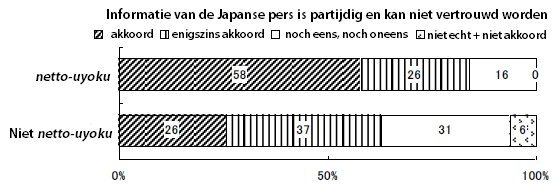
\includegraphics{images/tsuji_masukomi_translated.jpg}
\caption{(onder de versoepelde voorwaarden): geloofwaardigheid van
massamedia onder net rechtsen. (Bron: Tsuji
\protect\hyperlink{ref-tsujiux5fintanettoux5f2008}{2008}, 14)}
\end{figure}

In een online enquête\footnote{Om conclussies te kunnen trekken
  reduceerde Tsuji de resultaten tot een totaal van 998, met een gelijke
  verdeling tussen het aantal mannen en vrouwen, alsook het aantal
  mensen met een leeftijd tussen 20-24, 25-29, 30-34, 35-39 en 40-44.}
merkt Tsuji (\protect\hyperlink{ref-tsujiux5fintanettoux5f2008}{2008},
10--12) vooral bij mannen neigingen tot die karaktertrekken op. Ook ziet
hij een correlatie tussen een gevoel van eenzaamheid bij de deelnemers
en dat anti-Koreaans en/of anti-Chinees sentiment, iets dat volgens hem
misschien eerder aan de basis van dat sentiment ligt dan
nationalistische ideologieën. Leeftijd en onderwijs lijken echter geen
belangrijke rol te spelen. Ten slotte concludeert Tsuji wel dat slechts
1.3\% (13 mensen) van de deelnemers met alle stellingen uit de enquête
akkoord gingen en aldus aan alledrie de kenmerken van de net rechtse
stem voldeden.\footnote{36.8\% (367 mensen) voelden anti-Koreaans of
  anti-Chinees sentiment, 6.4\% (64 mensen) gingen akkoord met politiek
  conservatieve en nationalistische kwesties, en 15.2\% (152 mensen)
  maakten gebruik van computerondersteunde communicatie om
  maatschappelijke en politieke kwesties te bespreken (Tsuji
  \protect\hyperlink{ref-tsujiux5fintanettoux5f2008}{2008}, 11).} Om
meer betrouwbare resultaten te verwerven werden de voorwaarden om tot
die groep te horen iets uitgebreidt (tot deelnemers die akkoord gaan met
meer dan de helft van alle stellingen per karaktertrek), met als
resultaat een nieuw totaal van 31 personen. Uit die resultaten vindt
Tsuji twee andere kenmerken terug in berichten van net rechtsen: een
achterdocht jegens massamedia\footnote{Net zoals Rolfe en zijn idee van
  een anti-massamedia \emph{underground} \emph{netizen}-beweging
  argumenteert ook Akihiro Kitada dat het hele discours van 2channel
  ontstond uit een cynische kijk op massamedia (Itō, Okabe, en Tsuji
  \protect\hyperlink{ref-itoux5ffandomux5f2012}{2012}, hfst. 3).} (zie
\textbf{figuur 1}) en het frequent deelnemen aan internet
`\emph{flaming}' (炎上).\footnote{Het plaatsen van vijandelijke of
  beledigende berichten op internetdiscussies.}

\subsubsection{\texorpdfstring{Anti-Koreaans en/of anti-Chinees
sentiment (\emph{kenkan kenchū}
嫌韓嫌中)}{Anti-Koreaans en/of anti-Chinees sentiment (kenkan kenchū 嫌韓嫌中)}}\label{anti-koreaans-enof-anti-chinees-sentiment-kenkan-kenchux16b-ux5accux97d3ux5accux4e2d}

Xenofoob sentiment tegenover de Aziatische buurlanden omvat enerzijds
historische problemen (\emph{rekishi mondai} 歴史問題) en anderzijds
diplomatieke problemen (\emph{gaikōmondai} 外交問題). Onder historische
problemen komen vooral de `troostmeisjes'-discussie (\emph{ianfu}
慰安婦) en de `Slachting van Nanjing' (\emph{nankindaigyakusatsu}
南京大虐殺) sterk ter sprake. Diplomatische problemen omvatten dan weer
territoriale disputen en het afkoelen van relaties sinds dat plannen ter
hervorming van schoolboeken historische problemen begonnen te
bagatelliseren.

Negatief sentiment op het internet richt zich ook sterk reactionair
tegen de idee dat onderwijs in China, beide Korea's en Koreaanse scholen
in Japan anti-Japanse opvoeding (\emph{han'nichi kyōiku} 反日教育)
aanbiedt en aldus haat zaait onder diens inwoners. Net rechtsen delen
ook frequent door middel van alternatieve nieuwsbronnen en
video-uploadwebsites incidenten die `anti-Japanse' ideologieën zouden
meedragen, vaak met de boodschap dat mainstream media deze `waarheid
probeert te verbergen' (Yasuda
\protect\hyperlink{ref-yasudaux5fnettoux5f2012}{2012}; Taka
\protect\hyperlink{ref-takaux5ftwitterux5f2015-1}{2015}\protect\hyperlink{ref-takaux5ftwitterux5f2015-1}{a},
144).\footnote{In een kwantitatieve analyse van Japanse
  Twitter-berichten merkt Taka
  (\protect\hyperlink{ref-takaux5ftwitterux5f2015-1}{2015}\protect\hyperlink{ref-takaux5ftwitterux5f2015-1}{a})
  ook een frequent voorkomen van termen als `fabricatie' (\emph{netsuzō}
  捏造, 2,472 keer), `leugen' (\emph{uso} 噓, 2,170 keer) en
  `\emph{masugomi}' (マスゴミ, 1,290) die een wantrouwen jegens
  mainstream nieuwsgeving en massamedia aantonen.}

\paragraph{China}\label{china}

Een recent incident dat anti-Chinees sentiment online in de hand werkte
was het `Minjinyu 5179'-incident in 2010. Een aanvaring tussen een
Chinese vissersboot en twee Japanse kustvaartschepen op betwist gebied
nabij de Pinnacle-eilanden leidde tot het afkoelen van Sino-Japanse
diplomatieke betrekkingen en sterke discussies op het internet. De
terughoudendheid van de Japanse overheid om videomateriaal van dat
accident vrij te geven, alsook het ingaan op de eisen gesteld door
China, leidden tot ook antagonisering van de DPJ.

Ook wanneer toenmalig gouverneur van Tokyo Ishihara Shintarō in 2012
bekend maakte de Pinnacle-eilanden (een belangrijk pijnpunt in huidige
Sino-Japanse relaties) te willen overkopen en een online-crowdfunding
campagne opstartte, was het diezelfde stem die zich hier collectief bij
aansloot en aanzette tot donaties, met een uiteindelijke 1,485,201,967
yen\footnote{In 2012 kwam dit bedrag overeen met 14,067,361 euro.}
verzameld door 113,602 burgers (Hollihan
\protect\hyperlink{ref-hollihanux5fdisputeux5f2014}{2014}, 185; Horiuchi
\protect\hyperlink{ref-horiuchiux5fpublicux5f2014}{2014}, 36--38).

\paragraph{Noord-Korea}\label{noord-korea}

Japan's relaties met Noord-Korea zijn nooit formeel genormaliseerd. De
recente publieke perceptie in Japan is reeds overheersend
negatief\footnote{In een internationale enquête uitgevoerd in 2014 door
  BBC World Service werd Noord-Korea door 91\% van de Japanse bevolking
  als negatief bestempeld. Anderzijds is negatief sentiment jegens Japan
  in zowel Zuid-Korea en China sterk gestegen met een hoogtepunt van
  respectievelijk 79\% en 90\% (Poll
  \protect\hyperlink{ref-bbcux5fworldux5fserviceux5fpollux5f2014ux5f2014}{2014}).}
en stemt vooral uit de kidnappingskwestie van Japanse burgers eind jaren
'70 (die onder Koizumi in een normalisatiegesprek met Kim Jong-il in
2002 formeel erkend werd) en een aanhoudende militarisering. Specifiek
het nucleair wapenprogramma en het testen van langeafstandsraketten over
Japans territorium wekken nieuwe angst op.\footnote{Voor een beknopte
  analyse van bilaterale relaties tussen Japan en Noord-Korea verwijs ik
  naar Morris-Suzuki
  (\protect\hyperlink{ref-morris-suzukiux5fre-imaginingux5f2011}{2011}).}
Beide zaken worden dan ook uitvoerig online gediscussiëerd ter
versterking van (Noord-)Korea als de \emph{Ander} en leiden tot haat en
vooroordelen jegens iedereen of alles geassocieerd met Noord-Korea (Mie
\protect\hyperlink{ref-mieux5fxenophobiaux5f2013}{2013}; Itagaki
\protect\hyperlink{ref-itagakiux5fanatomyux5f2015}{2015}, 50).

\paragraph{Zuid-Korea}\label{zuid-korea}

Naast bovenstaande formele erkenning in 2002 beschrijft Itagaki
(\protect\hyperlink{ref-itagakiux5fanatomyux5f2015}{2015}) ook het 2002
FIFA wereldkampioenschap voetbal, georganiseerd door Japan en Zuid-Korea
ter bevordering van wederzijdse vriendschap en respect, als een keerpunt
in net rechtse perceptie van Zuid-Korea.\footnote{Na een overwinning van
  schaatskampioene Yu-Na Kim tegenover Asada Mao op de 2010 olympische
  winterspelen ontstond er een klein media-incident als gevolg van een
  cyberaanval op 2channel. Door een online lastercampagne die beweerde
  dat de jury werd omgekocht door de Zuid-Koreaanse overheid, hielden
  meer dan 10,000 Koreaanse \emph{netizens} op 1 maart 2010 een poging
  om 2channel stil te leggen. Die dag werd gekozen als verwijzing naar
  de \emph{Sam-il} (3·1) beweging in 1919, het eerste Koreaans protest
  tijdens de Japanse kolonisatie.} Online ontstond de perceptie dat
Zuid-Korea gebruik maakte van \emph{soft power}-middelen als populaire
cultuur om Japans territorium binnen te dringen en een anti-Japans
beleid door te voeren. Itagaki
(\protect\hyperlink{ref-itagakiux5fanatomyux5f2015}{2015}) beschrijft
dat fenomeen vervolgens als een vorm van cultureel racisme onder de
noemer `Korea-phobia' en traceert het historisch terug naar de
kolonisatie van Korea in 1910. Termen die historisch in een koloniaal
discours gebruikt werden om pejoratief te verwijzen\footnote{Een
  opvallend kenmerk van die termen zijn echter het gebrek van visuele of
  biologische kenmerken als bijvoorbeeld huidskleur. Ze vallen terug op
  vage elementen die niet op `raciaal' gebied een machtsrelatie uiten op
  cultureel of politiek gebied.} naar etnische Koreanen vonden ook hun
weg terug naar het online discours gehandhaafd door net rechtsen.
Voorbeelden van pejoratieve terminologie jegens etnische Koreanen zijn
legio, maar vooral historische termen \emph{futei senjin} (不逞鮮人,
opstandige koreanen) and \emph{sangokujin} (三国人, derdelandsonderdaan)
kennen een heropkomst nu gericht op de Koreaanse diaspora.

\paragraph{Koreaanse Diaspora}\label{koreaanse-diaspora}

De negatieve positie van de net rechtse stem tegenover de Zainichi (de
Koreaanse diaspora in Japan)\footnote{De zainichi-identiteit en
  discriminatie daartegen kent een lange, ingewikkelde geschiedenis.
  Voor een verdere uiteenzetting verwijs ik naar (Lie
  \protect\hyperlink{ref-lieux5fzainichiux5f2008}{2008}).} berust zich
voornamelijk op drie zaken: de speciale rechten die die diaspora zou
ontvangen in de vorm van onder andere sociale zekerheidsvoordelen en het
statuut als Speciale Permanente Inwoners,\footnote{Speciale Permanente
  Inwoners (\emph{tokubetsueijūsha} 特別永住者) zijn burgers in Japan
  met een speciaal statuut om permanent in Japan te verblijven. Het
  betreft vooral inwoners met een Koreaanse achtergrond die, na het
  Vredesverdrag van San Francisco in 1952, hun status als koloniale
  inwoners verloren en niet naturaliseerden als Japanse burgers.} het
gebruik van aliasen (\emph{tsūmei} 通名)\footnote{Gezien de onthulling
  dat de naam Sakurai Makoto zelf een alias is, kan in die kritiek een
  zekere ironie gelezen worden.} om zich te vermommen als `echte
Japanners', en een associatie met misdaad. Onder de naam \emph{zainichi
tokken} (Speciale Rechten voor Zainichi, 在日特権) zouden Koreaanse
inwoners van Japan genieten van zaken als belastingsverlaging, kosteloze
leningen, een hogere sociale uitkering, en andere bevoordeelde
behandelingen tegenover Japanners en andere buitenlandse inwoners
(Yasuda \protect\hyperlink{ref-yasudaux5fnettoux5f2012}{2012}).

Itagaki beschrijft de negativiteit ontstaan tegenover die ervaarde
bevoordeelde behandelingen als een ervaarde invasie van een verbeelde
Japanse ruimte. In net rechtse retoriek betekent positieve discriminatie
namelijk een verlies van rechten voor Japanners. Die logica waarin zaken
als mensenrechten tot schaarse goederen worden gereduceerd, komt overeen
met de logica van het economische \emph{zero-sum game} (nulsomspel)
model: de wij-groep dient evenveel rechten in als de zij-groep ontvangt
(\protect\hyperlink{ref-itagakiux5fanatomyux5f2015}{2015},
60).\footnote{Zie ook Morris-Suzuki
  (\protect\hyperlink{ref-morris-suzukiux5fbeyondux5f2015}{2015}). Zij
  vergelijkt dergelijke retoriek van `\emph{Zero-Sum Citizenship}' met
  die van extreem-rechtse groeperingen in Europa en de Verenigde staten,
  en stelt `\emph{Semi-Citizenship}' als theoretisch framework om
  dergelijke redenatie te overkomen.}

Afgaande op het model van digitaal populisme eerder opgesteld, wordt dat
idee verder in stand gezet door het digitaal verspreiden van valse
informatie (\emph{gasaneta} ガセネタ) en geruchten (\emph{dema} デマ,
\emph{ryūgen} 流言 of \emph{uwasa} うわさ). Yasuda
(\protect\hyperlink{ref-yasudaux5fnettoux5f2012}{2012}, 219) beschrijft
bijvoorbeeld het vaak voorkomend gerucht van een zogenaamde `Koreaanse
Bezettingsmacht' (\emph{chōsen shinchūgun} 朝鮮進駐軍), georganiseerde
Anti-japanse misdaad gepleegd door etnische Koreanen in Japan na de
Tweede Wereldoorlog. Ook na de aardbeving in 2011 deden er online
allerhande geruchten de ronde dat Zainichi Koreanen zich aan diverse
criminele activiteiten zouden hebben schuldig gemaakt.\footnote{Zie ook
  Ogiue (\protect\hyperlink{ref-ogiueux5fkenshoux5f2011}{2011}).}
Twitterberichten verzameld door een zekere \emph{mutsuo\_toi}
(\protect\hyperlink{ref-mutsuoux5ftoiux5fhigashinihonux5f2011}{2011}) op
een persoonlijke blog stellen dat er etnische Koreanen zijn overgegaan
tot moord, diefstal en verkrachting. In een ander blogbericht stelt
Yahoo! Japan gebruiker \emph{nanako\_1892}
(\protect\hyperlink{ref-nanakoux5f1892ux5fzainichikankokujinux5f2014}{2014})
bijvoorbeeld dat er misbruik gemaakt werd van de aardbeving om de
identiteit van gestorven of vermiste Japanners over te nemen.\footnote{Die
  geruchten kunnen echter sterke consequenties hebben. Na de Grote Kanto
  Aardbeving van 1923 ontstonden er geruchten dat Koreanen in Japan
  gebruik maakten van de situatie om rel te schoppen en drinkwater te
  vergiftigen. Die geruchten leidden tot een heksenjacht op Koreanen met
  minstens 6.000 doden als gevolg (Jooeun
  \protect\hyperlink{ref-jooeunux5fgreatux5f2011}{2011}).}

\subsubsection{Politieke Voorkeur}\label{politieke-voorkeur}

Op nationale schaal wordt de net rechtse stem vooral verbonden aan Abe
Shinzo en het nationalistisch beleid dat daar aan gekoppeld gaat. Murai
(\protect\hyperlink{ref-muraiux5fnetux5f2012}{2012}) analyseert
maandelijkse opiniepeilingen naar politieke voorkeuren gehouden op
video-uploadwebsite Niconico en merkt, wanneer vergeleken met
offlinecijfers, een sterkere neiging naar conservatisme en steun voor de
Liberaal-Democratische Partij (LDP), ten koste van de Democratische
Partij Japan (DPJ). Na het doorbreken van de machtspositie van de LDP
door de JDP in 2009 groeide er een anti-JDP sentiment op
internetgemeenschappen frequent geassocieerd met net rechts. Zij bekeken
de JDP als een anti-Japanse (\emph{han'nichi} 反日) partij bestaande uit
voornamelijk zainichi Koreanen die werken tegen het beste belang van een
homogene Japanse bevolking.

Een ander aspect van beide opiniepeilingen, aan de andere kant, levert
inzicht over de tevredenheid in politiek en toont een sterker
scepticisme bij online deelnemers. Murai trekt aldus de conclusie,
afgaande op de cijfers gehaald uit de internetgemeenschappen opgebouwd
rond Niconico en publieke opiniepeilingen, dat \emph{netizens} een
sterkere politieke bewustheid hebben dan leeftijdsgenoten die aan de
offline opiniepeiling deelnamen, maar anderzijds ook dat er onder
jongere mensen veel meer zwevende (\emph{fudō-hyō} 浮動票) dan vaste
kiezers (\emph{kotei-hyō} 固定票) voorkomen. Hij concludeert als volgt:

\begin{quote}
This is an ideal condition for Net Uyoku's ideology to pervade. When
susceptible people meet sensational videos, they may easily embrace the
advertised ideology.
(\protect\hyperlink{ref-muraiux5fnetux5f2012}{2012}, 371)
\end{quote}

\subsubsection{Internetcommunicatie}\label{internetcommunicatie}

De net rechtse beweging en rechts-nationalistische internetdiscussies in
Japan worden het meest in verband gebracht met online
communicatieplatformen 2channel en Niconico (Katayama
\protect\hyperlink{ref-katayamaux5f2-channelux5f2007}{2007}; Tsuji
\protect\hyperlink{ref-tsujiux5fintanettoux5f2008}{2008}; Rumi
\protect\hyperlink{ref-rumiux5fkoreansux5f2011}{2011}; Murai
\protect\hyperlink{ref-muraiux5fnetux5f2012}{2012}), maar recentlijk ook
Twitter (Yasuda \protect\hyperlink{ref-yasudaux5fnettoux5f2012}{2012};
Morris-Suzuki
\protect\hyperlink{ref-morris-suzukiux5ffreedomux5f2013}{2013}; Taka
\protect\hyperlink{ref-takaux5ftwitterux5f2015-1}{2015}\protect\hyperlink{ref-takaux5ftwitterux5f2015-1}{a}).
Alledrie behoren in 2017 tot de meest bezochte websites van Japan
(Alexa.com
\protect\hyperlink{ref-alexa.comux5ftopux5f2017}{2017}\protect\hyperlink{ref-alexa.comux5ftopux5f2017}{b}).\footnote{De
  top tien bestaat uit in afnemende mate uit zoekmachine google.co.jp,
  google.com, internetportaal Yahoo.co.jp, youtube.com, E-commercesite
  amazon.co.jp, Facebook, Twitter, bloghost-site FC2.co.jp, Wikipedia en
  E-commercesite Rakuten.co.jp. Niconico staat op de elfde positie, een
  daling van achtste positie in september 2015. 2channel staat op de
  achttiende positie.}

\paragraph{2channel}\label{channel}

2channel\footnote{In april 2017 kwam 95.8\% van het aantal bezoekers uit
  Japan, 2.2\% uit Zuid-Korea en 0.6\% uit China. Alexa statistieken
  stellen verder dat het publiek verschilt van de gemiddelde
  internetbezoeker met een sterke meerderheid aan mannen en bezoekers
  zonder (nog) enige vorm van hogere opleiding (Alexa.com
  \protect\hyperlink{ref-alexa.comux5ftopux5f2017}{2017}\protect\hyperlink{ref-alexa.comux5ftopux5f2017}{b}).}
is een anoniem internetforum opgericht in 1999 door een toenmalige
Japanse uitwisselstudent in de Verenigde Staten, Hiroyuki Nishimura, en
ervaarde een gestage groei tot grootste anonieme internetforum in Japan,
met in 2007 2.7 miljoen berichten per dag verspreid\footnote{Tien jaar
  later worden er nog ongeveer twee miljoen berichten per dag geplaatst
  (2ch.net \protect\hyperlink{ref-2ch.netux5fsuzumeux5f2017}{2017}).}
over 800 categoriëen (Katayama
\protect\hyperlink{ref-katayamaux5f2-channelux5f2007}{2007}). Enerzijds
blijkt het, door de anonimiteit en lakse regulering ervan, een geliefd
middel om op grassroots niveau politiek en media te discussiëren (Maslow
\protect\hyperlink{ref-maslowux5fnationalismux5f2011-1}{2011}).
Anderzijds resulteerde diezelfde lakse regulering echter wel in 50
civiele rechtszaken en meer dan vier miljoen dollar aan
schadevergoedingen of sancties voor zaken als laster en schending van
auteursrecht (Katayama
\protect\hyperlink{ref-katayamaux5f2-channelux5f2007}{2007}).

Door de grote schaal van het platform wordt 2channel geciteerd als
invloedrijk platform op vlak van mainstream opinievorming. Auteurs als
Rumi en Yasuda beschouwen het platform dan ook als voornaamste
communicatiemiddel van \emph{netizens} met ideologieën van de net
rechtsen,\footnote{Ook Tsuji
  (\protect\hyperlink{ref-tsujiux5fintanettoux5f2008}{2008}) leest in de
  resultaten van zijn enquête een correlatie tussen 2channel en
  rechtsnationalistisch gedachtengoed.} en brengen het ook in
rechtstreeks verband met het ontstaan van nationalistische
volksbewegingen als de Zaitokukai (Rumi
\protect\hyperlink{ref-rumiux5fkoreansux5f2011}{2011}; Yasuda
\protect\hyperlink{ref-yasudaux5fnettoux5f2012}{2012}). In een studie
over internetnationalisme observeert Rumi
(\protect\hyperlink{ref-rumiux5fkoreansux5f2011}{2011}) bijvoorbeeld een
\emph{thread}\footnote{Een specifieke conversatie die wordt opgestart op
  een internetforum (of andere vormen van internetcommunicatie) waarin
  gebruikers bijdragen tot discussie door het plaatsen van reacties.}
die een Koreaans webartikel over `Takeshima Day'\footnote{Om Japans
  aanspraak op de eilanden in het territoriaal dispuut rond de Liancourt
  Rocks te benadrukken houdt de Shimane-prefectuur een jaarlijkse
  viering op 22 februari. Op die dag werden de eilanden in 1905, tijdens
  de Russisch-Japanse oorlog, geannexeerd als Japans territorium en tot
  onderdeel van Shimane gemaakt.} discussieert. Op vier dagen tijd
werden er 7,000 berichten geplaatst die al snel inhoudelijk devieerden
van het oorspronkelijk onderwerp en herleid werden naar herhalingen van
typische net rechtse retoriek. Eerder dan discussie werd op dergelijke
manier het beeld van Koreanen als een geweldadige, irrationele Andere in
stand gehouden en versterkt; enige poging tot discussie zelf werd al
snel genegeerd of afgeschreven als berichten van anti-Japanse spionnen
(\protect\hyperlink{ref-rumiux5fkoreansux5f2011}{2011}, 5--8).

\begin{quote}
``Collectively, the 7,000 postings produced and reinforced the negative
image of Korea and Koreans far beyond the Tsushima issue. Forum
participants brought up a multitude of Korearelated issues which had
nothing to do with Korean tourists on Tsushima: the `special tax and
welfare privileges' that zainichi Koreans allegedly enjoy, the `illegal
occupation' of Takeshima Island', kimchi with parasite eggs, or crimes
by Koreans in Japan and overseas. Links were made to a TV news item
about a Japanese boy who was attacked in Korea, snapshots of
anti-Japanese artwork by Korean school children, a Youtube clip on a
rape by a zainichi Korean, 2-chan threads on zainichi pension
entitlement and welfare benefits, shocking images of anti-Japanese
demonstrators slaughtering pheasants (Japan's national bird) in front of
the Japanese Embassy, and many more. These and other unrelated events
and images are linked together under the unifying but empty sign of the
`Koreans'.'' (Rumi
\protect\hyperlink{ref-rumiux5fkoreansux5f2011}{2011}, p5)
\end{quote}

Een voorbeeld van nationalistische discussies gestart op 2channel die
zich offline uiten zien we in enkele protestacties die voor het eerst op
7 en 21 augustus 2011 werden gehouden aan het hoofdkantoor van Fuji
Television in Tokio (Itagaki
\protect\hyperlink{ref-itagakiux5fanatomyux5f2015}{2015}). Er ontstond
woede uit het idee dat Fuji Television, onder de stijgende populariteit
van Koreaanse pop-cultuur, voornamelijk Koreaanse drama's uitzond,
waardoor ze vervolgens werden bestempeld als een `\emph{traitor
network}'.\footnote{Fuji TV kwam in 2015 nogmaals onder vuur, op dat
  moment voor wat werd beschouwd als het opzettelijk haat zaaien tussen
  Zuid-Korea en Japan. Doormiddel van foutief gebruikte Japanse
  ondertitels van geïnterviewde Zuid-Koreanen in Japan onstond de
  perceptie dat de geïnterviewden `Japan haten' (Osaki
  \protect\hyperlink{ref-osakiux5ffujiux5f2015}{2015}).} Het aantal
deelnemers werd door verschillende online kranten, waaronder ook
Zuid-Koreaanse, tussen de 2,000 en 10,000 geschat (The Chosun Ilbo
\protect\hyperlink{ref-theux5fchosunux5filboux5fjapaneseux5f2011}{2011};
The Donga Ilbo
\protect\hyperlink{ref-theux5fdongaux5filboux5fjapansux5f2011}{2011};
Schilling \protect\hyperlink{ref-schillingux5fjapaneseux5f2011}{2011}),
maar had verder echter geen invloed op de programmatie van Fuji
Television. In die protesten diende Fuji Television uiteraard als object
ter representatie van een diepgewortelde ontevredenheid onder deelnemers
in Tokio. Dat tegenover een ervaren Zuid-Koreaanse \emph{soft-power}
dreiging in de vorm van de \emph{Korean Wave} enerzijds, en tegenover
massamedia en veronderstelde mediamanipulatie anderzijds. Die protesten
werden live uitgezonden op verschillende video-uploadsites, waaronder de
populaire Japanse Niconico.

\paragraph{Niconico}\label{niconico}

Niconico (ニコニコ),\footnote{Volgens Alexa Rank kwam in april 2017
  92.9\% van het internetverkeer uit Japan, gevolgd door 2.7\% uit
  China, 1.4\% uit Taiwan en 1.2\% uit Zuid-Korea. Vervolgens blijken
  Niconico bezoekers het meeste te overlappen met die van 2channel
  (Alexa.com
  \protect\hyperlink{ref-alexa.comux5fnicovideo.jpux5f2017}{2017}\protect\hyperlink{ref-alexa.comux5fnicovideo.jpux5f2017}{a}).}
in 2006 opgericht als Nico Nico Douga (\emph{Niko Niko Dōga}
ニコニコ動画), is een Japanse video-uploadwebsite met als specifiek
kenmerk de mogelijkheid tot het plaatsen van commentaar rechtstreeks op
het videoscherm zelf om een soort gemeenschappelijke kijkervaring te
bekomen. In 2015 verklaarden de ontwikkelaars een record van 50 miljoen
geregistreerde gebruikers en een extra 2,5 miljoen betalende gebruikers
te hebben overschreden (Nicovideo.jp
\protect\hyperlink{ref-nicovideo.jpux5fpuremiamuux5f2015}{2015}).

\begin{figure}[htbp]
\centering
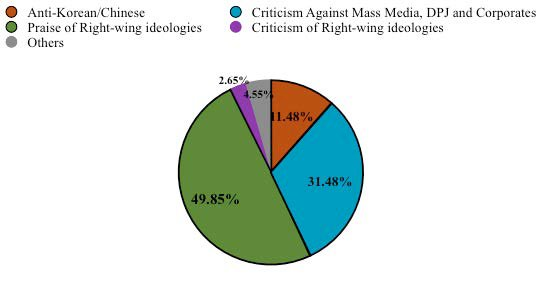
\includegraphics{images/murai_2012_nico.jpg}
\caption{Thematische categorisering van video's op de
`politics'-categorie van Niconico. (Bron: Murai
\protect\hyperlink{ref-muraiux5fnetux5f2012}{2012}, 370)}
\end{figure}

Hoewel Niconico vooral gericht is op populaire sub-culturen als die van
o.a. Japanse animatie en videospellen, met een doelpubliek overlappend
met 2channel, heeft het ook een actieve `\emph{Politics}' categorie. Die
categorie brengt Murai
(\protect\hyperlink{ref-muraiux5fnetux5f2012}{2012}) in verband met net
rechtse ideologiëen: onvrede jegens de DPJ, massamedia en
Oost-Aziatische landen als Zuid-Korea en China. Hij merkte na
kwantitatief onderzoek op dat 92.8\% (3712/4000) van het aantal
populairste videos in de categorie `politics' ideologieën van de net
rechtsen bevatten, met slechts 2.65\% (106/4000) videos die daar kritiek
op gaven (\protect\hyperlink{ref-muraiux5fnetux5f2012}{2012}, 370).
\textbf{Figuur 2} deelt dat verder onder.

\paragraph{Twitter}\label{twitter}

Ook in Japan is Twitter uitgegroeid tot een uiterst populaire vorm van
sociale media, met in 2001 een aandeel van 25\% van alle berichten op
Twitter geschreven in het Japans. Het net rechtse gebruikersbestand op
Twitter, vaak onder een koepelterm `Hinomaru factie' (\emph{hinomaru
kurasuto} 日の丸クラスト), kenmerkt zich enerzijds door een Japanse
vlag\footnote{De \emph{hinomaru} (日の丸) of officieel de
  \emph{nisshōki} (日章旗) is de officiële vlag van Japan. Een andere
  vaakgebruikte variant is de Rijzende Zon-vlag (\emph{Kyokujitsu hata}
  旭日旗), een vlag geassocieerd met oorlogsvoering tussen de
  Edo-periode en het einde van de Tweede Wereldoorlog, en in buurlanden
  met het Japanse militarisme.} op de profielfoto, vaak in combinatie
met militaire middelen en/of Japanse cartoonpersonages, en anderzijds
door de aan net rechtse verbonden retoriek in de introductiekolom van de
gebruiker (Hack
\protect\hyperlink{ref-hackux5fsubcultureux5f2016}{2016}).\footnote{Met
  variaties op `Ik hou van Japan' (\emph{nihon daisuki} 「日本大好き」)
  wordt vaak de liefde verklaard voor Japan, en met variaties van `ik
  ben simpelweg een in Japan geboren Japanner' (\emph{tan'naru Nihon
  umare no nihonjin} 「単なる日本生まれの日本人。」) wordt de
  nationalistische retoriek van de gebruiker genormaliseerd tot iets wat
  voor de hand liggend is voor een gewone Japanse burger.} Zie
\textbf{Figuur 3} voor voorbeelden daarvan.

\begin{figure}[htbp]
\centering

\includegraphics{images/twitter_hinomaru_crest.jpg}
\caption{Voorbeelden van `Hinomaru faction' Twitter-accounts. (Bron:
Twitter)}
\end{figure}

Taka Fumiaki stelt dat sociale media een belangrijke rol heeft gespeeld
in de groei van modern racisme\footnote{Ook wel symbolisch racisme, in
  tegenstelling tot ouderwets racisme, gebaseerd op werken van David
  Sears en John McConahay. Wordt samengevat tot vier punten: 1.
  Minderheden worden niet langer geconfronteerd met vooroordelen en
  discriminatie. 2. Ongelijkheid komt als gevolg voort uit een gebrek
  aan inspanning door die minderheden. 3. Zelfs dan nog stellen
  minderheden in een protest tegen discriminatie te veel eisen. 4.
  Minderheden hebben meer voorrechten gekregen dan dat ze verdienen
  (Taka
  \protect\hyperlink{ref-takaux5ftwitterux5f2015-1}{2015}\protect\hyperlink{ref-takaux5ftwitterux5f2015-1}{a},
  143).} en xenofobie in Japan. Om dat te onderzoeken voerde hij een
kwantitatieve tekstanalyse uit op een databank van Twitterberichten
handmatig opgehaald door middel van kernwoorden met betrekking op
Koreanen
(\protect\hyperlink{ref-takaux5ftwitterux5f2015-1}{2015}\protect\hyperlink{ref-takaux5ftwitterux5f2015-1}{a})
en China
(\protect\hyperlink{ref-takaux5ftwitterux5f2015}{2015}\protect\hyperlink{ref-takaux5ftwitterux5f2015}{b}).
Taka concludeert dat het merendeel van die berichten negatief
sentiment\footnote{Respectievelijk uit 109,589 berichten 70\% negatief
  sentiment tegenover Koreanen en uit 67,884 berichten 67.3\% negatief
  sentiment tegenover China.} bevat, vooral met betrekking tot misdaad,
speciale rechten, anti-Japans gedrag of corruptie in het politieke
landschap. Daarvoor wordt vaak gerefereerd naar alternatieve
nieuwsbronnen, met name verzamelblogs verbonden aan 2channel
(\emph{2-channeru matome burogu} 2ちゃんねるまとめブログ). Ten slotte
zijn discussies met betrekking tot Koreanen opvallend omvangrijker.

\subsection{Theoretische Benadering}\label{theoretische-benadering}

Net als Matsumura e.a.
(\protect\hyperlink{ref-matsumuraux5fdynamismux5f2005}{2005}), Murai
(\protect\hyperlink{ref-muraiux5fnetux5f2012}{2012}) en Rumi
(\protect\hyperlink{ref-rumiux5fkoreansux5f2011}{2011}) poogt deze paper
vanuit theoretisch perspectief een verklaring te geven aan het
nationalisme en de ideologische polarisatie die plaatsvind in de
anonimiteit van bovenstaande communicatieplatformen. Kiesler, Siegel, en
McGuire (\protect\hyperlink{ref-kieslerux5fsocialux5f1984}{1984}), en
Lea (\protect\hyperlink{ref-leaux5fsocialux5f1992}{1992}) zijn koplopers
op gebied van studies rond sociale en psychologische gevolgen uit
anonieme computerondersteunde communicatie. Zij toonden aan dat
anonimiteit een gebrek aan sociale verantwoordelijkheid en groepsvorming
gebaseerd op retoriek kan meebrengen, dat weer leidt tot verdere
groepspolarisatie. Deze paper, in een sociale identiteitsbenadering,
analyseert de net rechtse beweging als een verbeelde gemeenschap vanuit
recentere modellen die verder op bovenstaande theorieën bouwen.

\subsubsection{Verbeelde
(cyber)Gemeenschappen}\label{verbeelde-cybergemeenschappen}

In zijn onderzoek naar nationalisme bedacht Anderson
(\protect\hyperlink{ref-andersonux5fimaginedux5f2006}{2006}) de term
`verbeelde gemeenschap' (\emph{imagined community}), een sociale
constructie ter verklaring van een bindingsgevoel dat leidde tot
nationalisme vanaf de vroege negentiende eeuw. In een drang naar sociale
interactie worden, door categorisering, arbitraire overeenkomstigheden
gebruikt ter creatie van verbeelde gemeenschappen. Verbeeld, omdat leden
van gemeenschappen, hoewel ze elkaar nog ontmoet hebben, toch een gevoel
van eendracht bezitten en zich aldus als een relatief homogene groep
plaatsen tegen mensen buiten die groep. Anderson beschouwd de natiestaat
als een verbeelde gemeenschap omdat het bindingsgevoel onder leden
daarvan wordt geconstrueerd uit etnische afkomst en een nationale ethos.
In de creatie van een verbeelde gemeenschap spelen vooral het
printkapitalisme en het ontstaan van een gemeenschappelijke taal door
printmedia een primaire rol, aldus Anderson. De daaruit gegroeide
massamedia propageert binnen een vaak geografische afgebakende regio,
staatsgeleide, homogene narratieven van identiteit in de vorm van
gemeenschappelijke herinneringen.

Met de opkomst van het internet als nieuwe mediavorm argumenteert
Appadurai (\protect\hyperlink{ref-appaduraiux5fmodernityux5f1996}{1996},
hfstk. 3 - 4) dat die opkomst kan leiden tot creatie van nieuwe
transnationale, verbeelde gemeenschappen. Die gemeenschappen zouden
gebaseerd zijn op ideologie eerder dan op de natiestaat, en met
gehanteerde narratieven die afwijken van die voortgebracht uit
traditionele media. De eentaligheid van Japanse \emph{netizens}
limiteert echter de mogelijkheid tot transnationaliteit. Als enige
sociale markeerders in een anonieme sfeer (zoals die van 2channel)
worden taal en ideologie de belangrijkste bindingsmiddelen van net
rechts als verbeelde, cybergemeenschap (Murai
\protect\hyperlink{ref-muraiux5fnetux5f2012}{2012}, 375--76).

\subsubsection{SIDE-model}\label{side-model}

Er bestaan omtrend de impact van anonimiteit op groepsvorming en
mogelijke (negatieve) gevolgen daaruit, zoals afwijkend gedrag en
geweldpleging, verschillende theoretische modellen. De klassieke
deïndividuatietheorie stelt bijvoorbeeld dat anonimiteit door middel van
aanwezigheid in een menigte leidt tot een verlies van zelfbewustzijn en
aldus persoonlijke verantwoordelijkheid. Dat zou leiden tot
antinormatief gedrag.

De ontwikkeling van het internet en daarmee verbonden grootschalige
computerondersteunde communicatie geeft echter een nieuwe context van
anonimiteit en ideeën over sociale signalen. Lea en Spears
(\protect\hyperlink{ref-leaux5fcomputer-mediatedux5f1991}{1991}) en Lea
(\protect\hyperlink{ref-leaux5fsocialux5f1992}{1992}) ervaren
anonimiteit in de context van het SIDE-model (\emph{social identity
model of deindividuation effects}) als een minimale mogelijkheid om
individuele verschillen te markeren, en nuanceren dat er onder invloed
van de sociale identiteitstheorie\footnote{Die theorie stelt dat de
  identiteitservaring gebaseerd wordt op de perceptie van zichzelf
  binnen een groep, en van de groep collectief tegenover andere groepen.
  Eerst zal men zichzelf en anderen categoriseren in groepen. Vervolgens
  zal men aan de hand van die groepen zichzelf (en anderen)
  identificeren en zich conformeren naar het gedrag dat van die groep
  verwacht wordt. Tenslotte begint het process van vergelijken. Gevolgen
  daarvan zijn dat de groep waar men toe behoort, de in-groep (`wij'),
  ter verhoging van eigenwaarde, de andere groep zal discrimineren.}
geen sprake is van een echt verlies van zelfbewustzijn. Dat, aangezien
volgens die theorie identiteit mee opgebouwd wordt door
zelf-categorisering in verschillende groepen. Volgens het SIDE-model
veschuift de persoonlijke identiteit juist naar die van de menigte en
wordt er aldus een groepsmentaliteit gevormd. Het eerder beschreven
antinormatief gedrag wordt dan juist uitgevoerd op basis van wat wel
telt als normatief gedrag in die groep -- al zijn het zelfs
gemeenschappelijke ideeën die geen basis hebben in de realiteit.

Verder doorgetrokken stelt deze theorie dat, mits er reeds enige
affiniteit bestaat met de groep in kwestie, anonimiteit groepsidentiteit
zal opleggen en versterken, maar ook bepaald gedrag zal normaliseren.
Indien dat niet het geval is zal het omgekeerde effect plaatsvinden en
versterkt de persoonlijke identiteit als los van de groep.

\subsubsection{Referent Informational Influence
Theory}\label{referent-informational-influence-theory}

Groepspolarisatie wordt beschreven als de neiging om als groep extremere
opvattingen te hanteren dan wat een individu eerst als intentie had.
Daarrond bestaan verschillende modellen. De \emph{Social comparison
theory} stelt bijvoorbeeld dat leden beginnen met een gematigde mening
en, door het vergelijken met die van anderen, als middel tot
onderscheiding een iets extremer standpunt innemen dat toch overeenkomt
met dat van de groep. De \emph{informational influence theory} stelt
eerder dat groepspolarisatie het gevolg is van de overtuigingskracht van
argumenten van de meerderheid in een groep. In een groep met een
gelijkaardige meningen worden verschillende argumenten bovengehaald ter
ondersteuning, en voor leden die deze argumenten nog kenden zorgt dat
voor een verdere versterking van die mening.

Een derde model, de \emph{referent informational influence theory} (of
``\emph{the social identity theory of influence in groups}'') bouwt
verder op de zelf-categorisatietheorie\footnote{De
  zelf-categorisatietheorie stemt voort uit de sociale
  identiteitstheorie en analyseert de cognitieve processen in
  zelf-categorisatie door de vraag te stellen wanneer, waarom en op
  welke basis we ons eerder als groep categoriseren dan als individu,
  alsook wat de psychologische gevolgen daarvan zijn. Op basis van
  sociale categoriëen gevormd uit geobserveerde overeenkomstigheden en
  contrasten categorizeren we anderen, maar veranderen we ook onze
  representatie van die leden. Ze worden niet langer gezien als unieke
  individuen maar als een uiting van attributen uit die groep en werken
  dus stereotypering in de hand. Op eenzelfde wijze wordt ook gedrag als
  conformiteit of etnocentrisme verklaard.} en verklaart
groepspolarisatie als een psychologische conformiteit (eerder dan
naleving of gehoorzaamheid) aan waarden in een bepaalde \emph{in}-groep.
Dat wordt gedaan wanneer men zich sterk identificeert met de normen van
die groep en die aldus opneemt als deel van de eigen identiteit. Om
zichzelf tot het uiterste te differentiëren tot een \emph{out}-groep,
eerder dan tot onderscheiding in de \emph{in}-groep, wordt er echter een
extremer standpunt ingenomen dan wat gemiddeld telt. In die theorie is
het dus ook niet de inhoud van de argumenten die telt, maar de sociale
positie van zichzelf in de groep waar de informatie uit komt (Turner,
Wetherell, en Hogg
\protect\hyperlink{ref-turnerux5freferentux5f1989}{1989}).

Eun-Ju Lee, in haar studie over deïndividuatie en groepspolarisatie
binnen computerondersteunde communicatie
(\protect\hyperlink{ref-leeux5fdeindividuationux5f2007}{2007}), past het
SIDE-model toe in combinatie met de \emph{referent informational
influence theory}. Ze concludeert dat het gebrek aan sociale signalen en
herkenningsattributen als kenmerk van computerondersteunde communicatie
sociale categorisatie en groepsidentificatie in de hand werkt wat, in
het distantiëren tot de \emph{out}-groep, tot groepspolarisatie leidt.
Aan de hand van die bevindingen stelt ze dat politieke discussies
uitgevoerd op anonieme fora, waarin argumenten langs beide kanten een
contrast creëeren tussen \emph{in} en \emph{out}-groep,
groepspolarisatie meebrengen enerzijds om de sociale positie in de groep
te verduidelijken, en anderzijds om zich te distantiëren van de
\emph{out}-groep. In dat geval, vermoedt ze, kan de discussie een
verdeeldheid in stand houden en versterken, eerder dan tot een publieke
consensus te komen.

De exclusiviteit van het net rechtse discours is daar een rechtstreeks
gevolg van. Door het proces van groepspolarisatie wordt er een selectie
gemaakt van `goede', patriottische burgers met gemeenschappelijke morele
waarden en normen ter creatie van een ideologisch homogene gemeenschap.
Nationalisme en patriottisme worden als primaire, juiste ideologieën
aangenomen en de daaruit vloeiende taal dient als signaal ter
identificatie van gelijkgestemden. De ideologieën van de groep worden
enerzijds op een gelijk niveau gebracht doordat ze zich omwikkelen in
deze gemeenschap, en anderzijds worden de meningen ter bescherming van
de eigen groep versterkt als contrast met de \emph{out}-groep.
Tegenstanders komen in hun gebrek aan patriottisme collectief
anti-Japans over en worden aldus volledig genegeerd. Ook Murai stelt dat
groepspolarizatie kenmerkend is voor de ideologieën die net rechtsen
handhaven. Murai stelt dat, zelfs als dat niet zou leiden tot enige vorm
van (online) activisme, het discours als een spiraal zodanig groeit dat
het op normatieve wijze wordt overgenomen door anderen, die
oorspronkelijk nog geen conservatieve neigingen hebben maar wel
toesluiting zoeken tot de online gemeenschap (Murai
\protect\hyperlink{ref-muraiux5fnetux5f2012}{2012}, 373--74).

Dankzij de anonieme aard van internetcommunicatie, en de rol van het
internet als een \emph{volkswil 2.0}, kunnen extremistische
volksbewegingen niet alleen hun radicale aard verbergen, ook consensus
wordt op die wijze gecreëerd. Dat doen ze door in te spelen op de morele
waarden en homogene \emph{wij}-heid van Japanse \emph{netizens}, en door
het antagoniseren van zowel andere mediavormen (de rol van massamedia
als manipulatief en het bewust verbergen van waarheden), als van
kritische tegenstanders -- zij worden afgestempeld als Koreaanse
anti-Japanse spionnen. De wij-groep wordt overtuigd om actie te
ondernemen en waarheden over Japanse vijanden te verspreiden om anderen
te doen ontwaken. Op die wijze maken ze zichzelf zowel tot patriottische
burgers als tot activisten die dankzij het medium zonder moeite kunnen
participeren door bijvoorbeeld video's te delen of deel te nemen in
discussies.

\subsection{Conclusie}\label{conclusie}

De populariteit van bovenstaande platformen toont aan dat in de
anonimiteit van het internet, en meer specifiek platformen als 2channel
waar ook een gebruikersnaam als herkenningsmiddel vermeden wordt, het
toch mogelijk is een gevoel van gemeenschap te creëren ondanks een
gebrek aan fysieke kenmerken. Dat wordt verklaard door een
gemeenschappelijke identiteit als patriottische \emph{netizens}, met
enerzijds de nativistische intentie om slechte anti-Japanse invloeden af
te weren en anderzijds ook een antagonisering van tegengestelde
meningen. Omdat er geen andere kenmerken ter herkenning zijn wordt dat
imago geheel opgebouwd uit de schrijfstijl en opbouw van geplaatste
berichten. Naar bovenstaande logica worden \emph{netizens}, aan de hand
van de ideologieën die in de anonieme berichten voorkomen, dan ook
geklassificeerd als ofwel patriottische \emph{netizens} ofwel
`anti-Japanse' vijanden (Murai
\protect\hyperlink{ref-muraiux5fnetux5f2012}{2012}, 374).

Met Mudde (\protect\hyperlink{ref-muddeux5foxfordux5f2013}{2013}) en
Lindgren (\protect\hyperlink{ref-lindgrenux5fdevelopingux5f2015}{2015})
in gedachten definieerde deze paper in het eerste deel aan de hand van
eerder onderzoek Japans populisme en bracht het in verband met
internetcommunicatie en sociale media. In het tweede deel werd verder
ingegaan op mogelijke sociale effecten van internetcommunicatie op de
maatschappij door als case-study de extreem-rechtse, nationalistische
internet-stem te nemen en diens politieke beweegredenen te bekijken. Het
tweede deel concludeert dat het internet in een creatie van
\emph{imagined cybercommunities} zowel polariseert als nationalistische
retoriek normaliseert, en aldus vrij spel creëert voor populisten.
Samenvattend voldoen de ideologieën die de net rechtsen voorhanden
hebben in grote lijnen aan de eerder opgestelde definitie van populisme.
Als gevolg van historische ontwikkelingen zijn ze inhoudelijk echter
vaak nativistisch door buitenlandse invloeden als anti-Japans te
plaatsen, en autoritair door de intentie die anti-Japanse invloeden te
straffen. In lijn met Rolfe
(\protect\hyperlink{ref-rolfeux5freinventionux5f2016}{2016}) worden
daarnaast ook, inherent aan het \emph{netizens}-discours, massamedia
afgeschilderd als de manipulatieve elite. Dit hoofdstuk plaatste de net
rechtse \emph{netizen}-groep als wij-groep of \emph{heartland} in
functie van populistische politici. In het laatste deel onderneemt deze
paper een poging om de ideologieën van Sakurai Makoto te classificeren:
iemand die zich opstelt als representatief voor die groep, en in de
literatuur daar vaak aan verbonden wordt.

\newpage

\section{Sakurai Makoto
(桜井誠)}\label{sakurai-makoto-ux685cux4e95ux8aa0}

Het hoeft niet gezegd te worden dat als spilfiguur in de discussie rond
hatespeech in Japan Sakurai Makoto een controversieel figuur is in het
Japanse medialandschap. Als zelfverklaarde internet-activist en
oprichter van de Zaitokukai haalt hij frequent het nieuws door
aaneenhoudende conflicten met o.a. de Koreaanse diaspora, en na een
aanklacht leidde dat in 2014 zelfs tot een veelbesproken publiek debat
met Hashimoto Tōru.\footnote{Enkele maanden eerder oordeelde een
  rechtbank in Osaka dat de haatdragende protestacties van de Zaitokukai
  onwetting waren. Op aandringen ging Hashimoto akkoord met het debat,
  maar na enkele minuten ging het debat over in een scheldpartij langs
  beide kanten.} Na een eerste poging om tot het politieke landschap van
japan toe te treden tijdens de Tokio 2016 gouverneursverkiezingen,
besloot hij een onafhankelijke partij op te richten met de Tokio
districtsverkiezingen van 2 juli 2017 op het oog: de Japan First Party.

\subsection{Achtergrond}\label{achtergrond}

Volgens een uitgebreid interview met de conservatieve centrum-rechtse
krant Sankei News in 2016 groeide Sakurai, geboren op 15 februari 1972,
vaderloos op in Fukuoka, waar hij studeerde aan Fukuoka Kenritsu Nakama
High School, tot hij in Edogawa, Tokio ging werken als part-time
administratief bediende. In dat interview haalt hij enkele anekdotes
naar boven die zijn huidige politieke ideologieën zouden hebben bepaald.
Voorbeelden omvatten een geschiedenisleerkracht die frequent vrijaf nam
om deel te nemen aan vakbondsacties van de Japan Teachers'
Union,\footnote{De Japan Teachers' Union (\emph{nihonkyoshokuinkumiai},
  日本教職員組合), Afgekort als JTU of \emph{nikkyōso} (日教組),
  functioneert als grootste onderwijsvakbond in Japan en neemt een
  kritisch standpunt in tegen het conservatieve beleid onder de LDP.}
studenten uit een school geaffillieerd aan Noord-Korea\footnote{\emph{Chōsen
  gakkō} (朝鮮学校) zijn Koreaanse scholen opgericht voor de Koreaanse
  diaspora in Japan, gesubsidieerd door Chongryon, een organisatie
  gekoppeld aan Noord-Korea.} die frequent geweld zouden plegen of
andere studenten bedreigden voor geld (Sankei News
\protect\hyperlink{ref-sankeiux5fnewsux5ftokyochiji-senux5f2016-1}{2016}\protect\hyperlink{ref-sankeiux5fnewsux5ftokyochiji-senux5f2016-1}{b}),
en lokale politici die stemmen omkochten door het sociale
zekerheidssysteem te misbruiken.

Als startpunt voor zijn anti-Koreaanse activiteiten (\emph{kenkan
katsudō} 嫌韓活動) geeft hij echter een anekdote over zijn ervaring op
een digitaal forum tijdens het FIFA wereldkampioenschap voetbal in 2002
georganiseerd in Seoul, Zuid-Korea. Ondanks volgens hem massale steun
voor Zuid-Korea vanuit Japan kwam er toch anti-Japans sentiment uit
Zuid-Koreaanse hoek (\emph{Nihon makero} 日本負けろ, `verlies, Japan!').
Vervolgens stelt hij dat Zuid-Koreanen geen genoegen nemen met het
1964-verdrag (dat de relatie tussen Zuid-Korea en Japan
normaliseerde)\footnote{Treaty on Basic Relations between Japan and the
  Republic of Korea (\emph{Nikkankihonjōyaku}, 日韓基本条約), getekend
  op 22 juni 1965.} en zaken als het `troostmeisjes-probleem' onnodig
laten aanslepen.

\begin{quote}
``Na dat drie jaar te hebben volgehouden {[}het online discussiëren met
Zuid-Koreanen{]} zei ik hun op het moment van mijn laatste discussie het
volgende: `Jullie stellen dat Koreanen {[}onder Japans colonialisme{]}
massaal werden geëxecuteerd. Waarom verdubbelde de bevolking dan tijdens
de annexatie?' Die cijfers staan in Zuid-Koreaanse schoolboeken hoor! In
schoolboeken door de Koreaanse overheid gepubliceerd! Daarom liet ik die
schoolboeken aan hun zien. Ik kreeg het volgende antwoord: `Nee, het
Japans Keizerrijk deed de bevolking stijgen om slaven te maken.' Toen
was ik uitgeput. Nu is het genoeg, ik kan niet verder blijven
argumenteren.'' (Sankei News
\protect\hyperlink{ref-sankeiux5fnewsux5ftokyochiji-senux5f2016-1}{2016}\protect\hyperlink{ref-sankeiux5fnewsux5ftokyochiji-senux5f2016-1}{b})
\end{quote}

\subsection{Activisme}\label{activisme}

Onder de gebruikersnaam \emph{konkon} begon Sakurai zijn anti-Koreaanse
internetactiviteiten, als iemand uit de net rechtse beweging, in 2002 op
een vertaalforum\footnote{Een vertaalforum (\emph{hon'yaku keijiban}
  翻訳掲示板) is een forum met achterliggende software die berichten op
  machinale wijze automatisch vertaalt naar de taal van de gebruiker.}
van de Zuid-Koreaanse krant `JoongAng Ilbo'. Vervolgens ging hij onder
zijn huidige gebruikersnaam \emph{Doronpa} over naar een vertaalforum
van Zuid-Koreaans internetportaal NAVER in 2003, en naar een van `Go
Korea' in 2004. Zijn frequente berichtgeving werd positief geëvalueerd
onder net rechtsen en leidde vervolgens tot het oprichten van zowel een
eigen site `Zuid-Korea, het vreemde land' (\emph{fushigi no kuni no
kankoku} 「不思議の国の韓国」)\footnote{Een woordspeling op het boek
  ``Alice in Wonderland'' (\emph{Gushigi no Kuni no Arisu}
  「不思議の国のアリス」)} als een forum genaamd `live discussie over
Korea' (\emph{Kankoku nama tōron} 「韓国生討論」). In januari 2005 werd
hij als gast van een publiek \emph{panel} gevraagd op een Nippon TV
(日本テレビ) \emph{variety}-programma `Generation Jungle'
(\emph{jenejan} 「ジェネジャン」) om vervolgens periodiek door Channel
Sakura uitgenodigd te worden.

Onder die nieuwverworven populariteit richtte hij in april 2005 een
rechtse volksbeweging op onder de naam `Onderzoeksgroep over het
probleem van de Japans-Koreanse geschiedenis' (\emph{Nikkan rekishi
mondai kenkyūkai}「日韓歴史問題研究会」),\footnote{Werd in 2006 hernoemd
  tot `Onderzoeksgroep over het probleem van Oost-Azië' (\emph{higashi
  ajia mondai kenkyūkai} 東亜細亜問題研究会).} met een eerste symposium
`het uit de hand gelopen anti-Japanse Zuid-Korea' (\emph{Bōsō suru
Kankoku no han'nichi} 「暴走する韓国の反日」) datzelfde jaar in juli.
Participatie daarvan wordt op ongeveer vijftig leden geschat. Periodieke
symposia, lezingen en zogenaamde studiegroepen leidden tot een stijging
van volgers en met enkele volgers startte hij vervolgens een eigen
internet-radioshow.

In december 2005 begon hij een carrière als schrijver met zijn eerste
eerste boek `Haat jegens de Korean Wave, een praktisch handboek: een
handleiding om ondoordachte Anti-Japanse opmerkingen af te weren'
(\emph{Kenkanryū jissen handobukku han'nichi mōgen gekitai manyuaru}
「嫌韓流 実践ハンドブック 反日妄言撃退マニュアル」) gepubliceerd door
uitgever Shinyusha Co., Ltd. (晋遊舎).\footnote{Door Yamano Sharin werd
  onder dezelfde uitgever ook de controversiële \emph{Manga Kenkanryu}
  (マンガ 嫌韓流, `Haat voor de Korean Wave') en \emph{Manga
  Kenchugokuryu} (マンガ嫌中国流, `Haat voor de Chinese Wave')
  uitgebracht.} Onder Seirindō (青林堂)\footnote{Een uitgever die vooral
  bekend staat voor de publicatie van de maandelijkse avant-garde manga
  Garo (ガロ).} en Shinyusha en bracht hij vervolgens zowel
solo-publicaties uit als contributies tot bestaande magazines als
\emph{Japanism} (「ジャパニズム」) (Yasuda
\protect\hyperlink{ref-yasudaux5fnettoux5f2012}{2012}).

\subsection{Zaitokukai}\label{zaitokukai}

Sakurai richtte de groep in 2006 op als protest jegens de zainichi
Koreanen, de Koreaanse diaspora in Japan, die misbruik zouden maken van
een oneerlijk systeem van sociale zekerheid ter compensatie van door
Koreanen gefabriceerde oorlogsmisdaden in de Tweede Wereldoorlog. Uit
een patriottisch idee om dergelijk anti-Japans gedrag te bestrijden en
Japan terug in handen van `echte Japanners' te geven houdt de groep
frequent protestacties (Yasuda
\protect\hyperlink{ref-yasudaux5fnettoux5f2012}{2012}; Murai
\protect\hyperlink{ref-muraiux5fnetux5f2012}{2012}, 373). Sakurai
weigert echter vergelijkingen met neo-nazisme en racistische
ideologieën, en verduidelijkt de groep te hebben gebaseerd op de
Noord-Amerikaanse Tea Party na het analyseren van diens campagnevideos.
Dat doet hij omdat hij op zelfde wijze overtuigd is dat Japan door de
invloed van linkse politici, media en buitenlanders een verkeerde
richting opgaat (Fackler
\protect\hyperlink{ref-facklerux5fnewux5f2010}{2010}).

\textbf{7 campagnepunten}

\begin{quote}
\begin{enumerate}
\def\labelenumi{\arabic{enumi}.}
\tightlist
\item
  ``De Zaitokukai laat de eis naar speciale voorrechten voor zainichi
  Koreanen die met `discrimatie' zwaaien, absoluut niet toe.''
\end{enumerate}
\end{quote}

\begin{quote}
\begin{enumerate}
\def\labelenumi{\arabic{enumi}.}
\setcounter{enumi}{1}
\tightlist
\item
  ``We voeren actief een verspreiding van kennis uit over het
  zainichi-probleem door van allerlei media gebruik te maken zoals het
  uitbreiden van onze officiële site, in verschillende regio's lezingen
  houden, enzovoort.''
\end{enumerate}
\end{quote}

\begin{quote}
\begin{enumerate}
\def\labelenumi{\arabic{enumi}.}
\setcounter{enumi}{2}
\tightlist
\item
  ``Als er vanuit bepaalde plekken een vraag komt naar een spreker, zal
  de Zaitokukai er voor zover mogelijk op reageren en, ongeacht de
  schaal van de bijeenkomst, een spreker uitzenden.''
\end{enumerate}
\end{quote}

\begin{quote}
\begin{enumerate}
\def\labelenumi{\arabic{enumi}.}
\setcounter{enumi}{3}
\tightlist
\item
  ``Met doelen als `pertinent tegen de speciale voorrechten voor de
  zainichi Koreanen' en `we laten het zainichi-probleem niet over aan de
  volgende generaties' zullen we het aansluiten aan de Zaitokukai sterk
  aanmoedigen.''
\end{enumerate}
\end{quote}

\begin{quote}
\begin{enumerate}
\def\labelenumi{\arabic{enumi}.}
\setcounter{enumi}{4}
\tightlist
\item
  ``Zodra we ons huidig doel van 10.000 geregistreerde leden hebben
  bereikt, starten we een petitie gericht naar de politieautoriteiten,
  gerechtelijke instanties, lokale overheden, politici, enzovoort, om
  tot een resultaat te komen van het zainichi-probleem.''
\end{enumerate}
\end{quote}

\begin{quote}
\begin{enumerate}
\def\labelenumi{\arabic{enumi}.}
\setcounter{enumi}{5}
\tightlist
\item
  ``Als er langs de kant van zainichi Koreanen een wens bestaat, zullen
  we via allerlei media als publicaties, uitzendingen, enzovoort,
  reageren met een openlijk debat.''
\end{enumerate}
\end{quote}

\begin{quote}
\begin{enumerate}
\def\labelenumi{\arabic{enumi}.}
\setcounter{enumi}{6}
\tightlist
\item
  ``De Zaikokai streeft naar het helpen om de werkelijke staat van
  plaatsen die lijden onder misdadig gedrag van opstandige zainichi
  Koreanen bekend te maken.''
\end{enumerate}
\end{quote}

(Zaitokukai.info
\protect\hyperlink{ref-zaitokukai.infoux5fzaitokukaiux5f2017}{2017})

\subsubsection{Demografie}\label{demografie}

In 2017 heeft de Zaitokukai naast het hoofdkantoor 36 afdelingen
verspreid over Japan. Een interactieve kaart op de officiële pagina van
de Zaitokukai (zie \textbf{figuur 4}) weergeeft per regio de demografie
van het ledenbestand. Indien die kaart up-to-date wordt gehouden omvat
het totaal aantal gebruikers op april 2017 volgens de organisatie 16399
leden,\footnote{Het totaal bevat een discrepantie van exact tien leden
  wanneer het vergeleken wordt met het opgetelde totaal (16,389 leden)
  van alle regio's in de interactieve kaart zelf.} waarvan 14079
(85,85\%) mannen en 2315 (14,12\%) vrouwen. Volgens \textbf{figuur 5}
zou het hoogst aantal leden komen uit Tokio (2945 leden of een 17,97\%
aandeel), gevolgd door Kanagawa (1313 leden of 8,01\%) en Osaka (1464
leden of 8,93\%).

\begin{figure}[!htb]
  \centering
    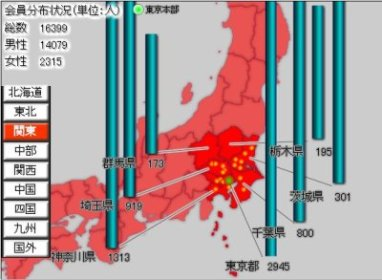
\includegraphics[width=.8\textwidth]{images/zaitokukai_user_base.jpg}
    \caption{Screenshot van het ledendistributiediagram van de Zaitokukai. (Screenshot genomen op 18/04/2017 om 13:35)}
\end{figure}

\begin{figure}[!htb]
  \centering
    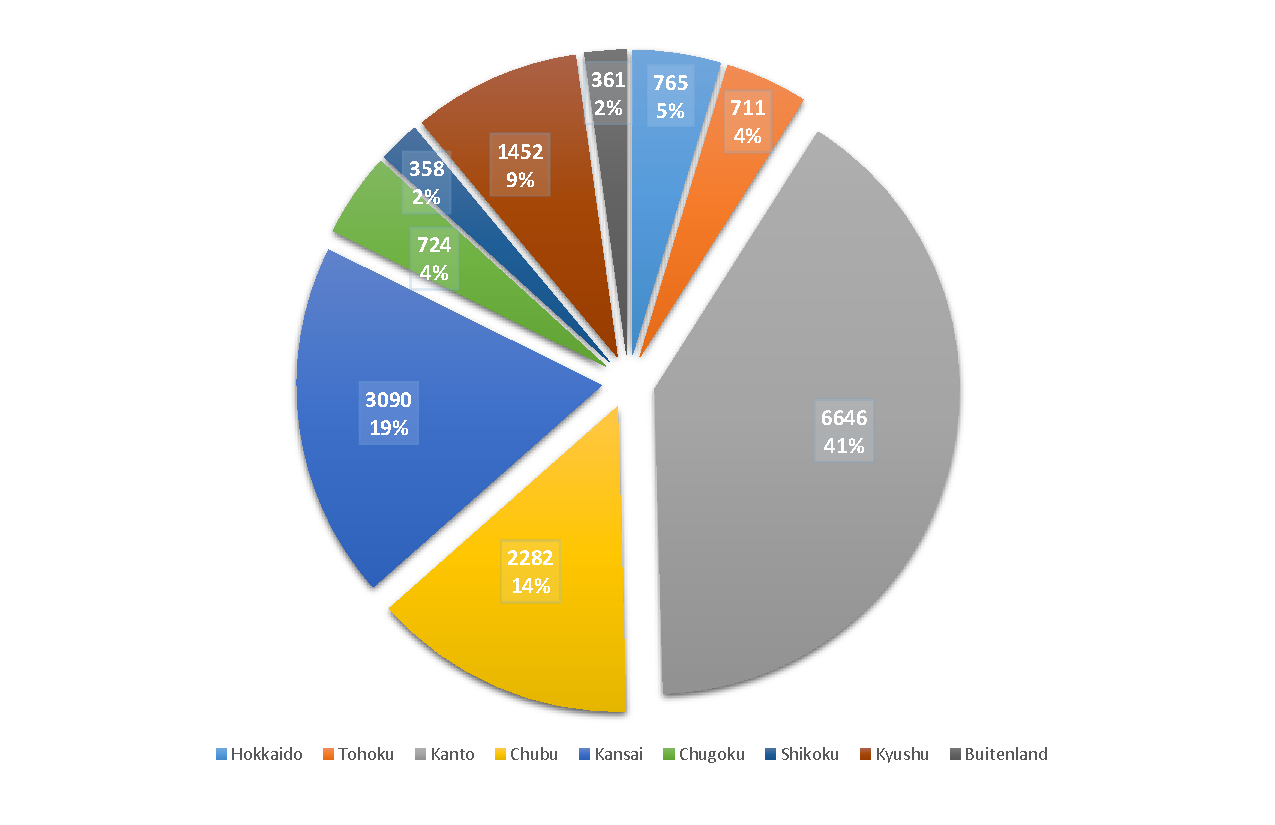
\includegraphics[width=.8\textwidth]{images/Zaitokukai_members.pdf}
    \caption{Cirkeldiagram van het aantal leden per regio.}
\end{figure}

\subsubsection{Betogingen}\label{betogingen}

Betogingen staan vooral in teken van eerdergenoemde speciale rechten
voor zainichi Koreanen, maar ook tegen andere ervaarde anti-Japanse
elementen wordt geprotesteerd. In 2011, na de kernramp van Fukushima,
hield Sakurai bijvoorbeeld een protestactie genaamd `Betoging om het het
Vuur van Nucleaire Reactoren Niet te Laten Doven' (\emph{Genpatsu no hi
o kesasenai demo kōshin} 「原発の火を消させないデモ行進」) als reactie
op antikernenergiebewegingen, wat live werd uitgezonden op Niconico. Hij
deed dat uit geloof dat die bewegingen zijn opgericht uit anti-Japans
sentiment, met de intentie om een tekort aan stroom te bekomen en aldus
Japan te verzwakken (Sakurai
\protect\hyperlink{ref-sakuraiux5fnihonux5f2011}{2011}).

In 2009 haalde de Zaitokukai voor het eerst sterke kritiek over zich
door een protestactie tegen het verblijf van een illegale Filipijnse
middelbare studente die in Japan mocht verblijven onder een speciaal
statuut.\footnote{Het was tevens de eerste protestactie van de
  Zaitokukai die een tegenprotest langs linkse kant uitlokte en een
  startpunt in de ontwikkeling van nieuwe sociale tegenwegingen
  (Shibuichi
  \protect\hyperlink{ref-shibuichiux5fstruggleux5f2016}{2016}).} In een
2009 protest tegen het illegaal gebruik van een openbaar park door een
\emph{chōsen gakkō}\footnote{\emph{Chōsen gakkō} (朝鮮学校) zijn
  Koreaanse scholen opgericht voor de Koreaanse diaspora in Japan,
  gesubsidieerd door Chongryon, een organisatie gekoppeld aan
  Noord-Korea.} lagere school als oefenterrein, organiseerde de
Zaitokukai op aanvraag van lokale inwoners, in samenwerking met
ultranationalistische volksbewegingen Shukenkai en Team Kansai een
betoging voor de poorten van de school. Door het roepen van racistische
en haatzaaiende slogans werden enkele leden aangeklaagd wegens
obstructie van openbare orde en laster met een boete van 12 miljoen yen
tot gevolg.\footnote{Het verdict werd op 9 december 2014 uitgesproken.
  De school zelf werd voor 100,000 yen beboet en werd voor
  veiligheidsredenen in 2012 gesloten.} Yasuda, in een interview met die
lokale inwoners, rapporteert anderzijds wel een dankbaarheid om het
probleem, al was het op extreme wijze, in de kijker te brengen (Yasuda
\protect\hyperlink{ref-yasudaux5fnettoux5f2012}{2012}), wat kan duiden
op een bepaalde reputatie van vigilantisme.

Ook in een protest tegen een fundraising gehouden door de
onderwijsvakbond in Tokushima ten voordele van arme jongeren hield de
Zaitokukai een betoging, op dat moment in het kantoor van de vakbond
zelf. Dat deden ze omdat een deel van het geld gedoneerd werd aan een
\emph{chōsen gakkō}. Het resultaat was een aanklacht en boete van 4,36
miljoen yen. In augustus 2014 volgde er een aanklacht wegens laster en
racisme door freelance-auteur en anti-hatespeech activiste Lee Sinhae.
Ze klaagde respectievelijk de Zaitokukai en een blog gerelateerd aan
2channel aan voor 5,5 miljoen yen en 22 miljoen yen. De zaak wordt
momenteel nog onderzocht.

\subsubsection{Reactie}\label{reactie}

In 2012 sprak een LDP-kandidaat\footnote{Advocaat Okazaki Akira
  (岡崎晃), op aanbeveling van de Komeito een kandidaat in het twaalfde
  district van Hyogo. Hij verloor met een tweede plaats tegen toenmalig
  regerend DPJ-lid Yamaguchi Tsuyoshi (山口壮).} zich op Twitter nog
positief uit over de groep (Okazaki
\protect\hyperlink{ref-okazakiux5ftwitterux5f2012}{2012}). Ook leden van
`The Party for the Japanese Kokoro' (\emph{Nippon no kokoro}
日本のこころ, oorspronkelijk `The Party for Future Generations',
\emph{Jisedai no tō} 次世代の党) en de `Osaka Restoration Association'
(\emph{Ōsaka ishin no kai} 大阪維新の会) spraken steun uit, maar die
werd later weer teruggetroken. Door die aaneenloping van bovenstaande
accidenten besloot Osaka burgemeester Hashimoto Tōru echter een
opiniemeeting te houden met Sakurai Makoto, wat uitmondde in een
scheldpartij langs beide kanten (2021 summer
\protect\hyperlink{ref-2021ux5fsummerux5fhashimotoux5f2014}{2014}).
Tijdens een live broadcast op Niconico verklaarde Sakurai in 2014 dat
hij zich als president zou terugtrekken\footnote{Sakurai Makoto beweert
  tevens vlak voor hij uit de Zaitokukai stapte, een uitnodiging te
  hebben ontvangen om naar een congres van nationalistische bewegingen
  als de Griekse Golden Dawn in Budapest te komen. Hoogstwaarschijnlijk
  gaat het over een geplande `National Policy Institute Conference' dat
  gepland werd in Budapest maar grondwettelijk werd tegengehouden en
  leidde tot een deportatie van NPI-oprichter Richard Spencer (Sankei News
  \protect\hyperlink{ref-sankeiux5fnewsux5ftokyochiji-senux5f2016-1}{2016}\protect\hyperlink{ref-sankeiux5fnewsux5ftokyochiji-senux5f2016-1}{b}).}
na het beëindigen zijn ambtstermijn\footnote{Vice-president Yagi
  Yasuhiro (八木康洋) heeft sindsdien telkens de Zaitokukai
  presidentsverkiezingen gewonnen en dient als huidig president.} om zo
meer tijd te hebben om nieuwe jonge conservatieve politici beter te
ondersteunen.\footnote{In 2016 richtte hij om die reden de `Beweging van
  Actief-Conservatieven' (\emph{kōdō suru hoshu undō}
  「行動する保守運動」) op.}

In december 2015 komt het Ministerie van Justitie, na een eerder vermeld
onderzoek naar hate speech, tot het besluit dat de opnames van
Zaitokukai-acties jegens zainichi Koreanen aanleiden tot haat en
racisme, en aldus in overtreding treden met mensenrechten. Het
ministerie vorderde daarom een eis uit aan Niconico en dergelijke
video-uploadsites tot verwijdering van deze videos. In mei 2016 voerde
het ministerie in een eerste poging om hate speech te bestrijden de
`Hate Speech Act of 2016' door, met voorbeelden van hatespeech verspreid
naar ongeveer 70 lokale overheden in maart 2017 (Times
\protect\hyperlink{ref-theux5fjapanux5ftimesux5fjusticeux5f2017}{2017}).

\subsubsection{Internet}\label{internet}

\begin{figure}[htbp]
\centering
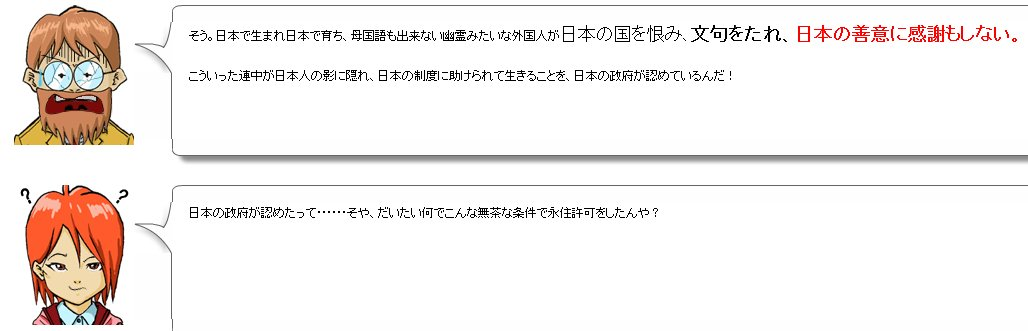
\includegraphics{images/zaitokukai_site_qa.jpg}
\caption{screenshot van een `vragenronde' over speciale rechten voor
Zaitokukai. (Bron: Zaitokukai.info
\protect\hyperlink{ref-zaitokukai.infoux5fzaitokukaiux5f2017}{2017})}
\end{figure}

Zaitokukai maakt sterk gebruik van sociale media en het internet. Naast
verschillende actieve accounts op Twitter, Facebook, enzovoort worden
activiteiten vaak live uitgezonden of achteraf geplaatst op
video-uploadsites als Niconico,\footnote{Dwango, het bedrijf achter
  Niconico, heeft onder invloed van de nieuwe wetgeving Zaitokukai's
  Niconico-account geblokkeerd (Furuya
  \protect\hyperlink{ref-furuyaux5fcanux5f2016}{2016}).} Channel Sakura
en Youtube.

De huigige webpagina heeft een eigen discussieruimte toegankelijk tot
geregistreerde leden, en hanteert een gelijkaardige visuele stijl aan
die van 2channel, met een toegankelijke, zelfs schattig design (zoals
een banner die lijkt op de profielfoto's gebruikt door de `Hinomari
clique' op Twitter). In de vorm van een cartoonesque Q\&A sessie (zie
\textbf{figuur 6}) tussen een fictieve professor en een zainichimeisje
\emph{Zaiko-chan} (ザイ子ちゃん) beschrijft een gids ten slotte de
voornaamste punten van de Zaitokukai.

\subsubsection{Strategie}\label{strategie}

Volgens Higuchi
(\protect\hyperlink{ref-higuchiux5fjapansux5f2014}{2014}\protect\hyperlink{ref-higuchiux5fjapansux5f2014}{a})
werft de Zaitokukai potentiële leden aan door net rechtsen te
contacteren die frequent anti-Koreaanse berichten plaatsen, of door een
latent wantrouwen jegens buitenlanders naar buiten te brengen met
haatwekkende videos. In Higuchi
(\protect\hyperlink{ref-higuchiux5fned:ux5f2014}{2014}\protect\hyperlink{ref-higuchiux5fned:ux5f2014}{b})
legt hij door middel van interviews een verdere band tussen activisten
en het internet. In die interviews blijken leden in aanraking te komen
met rechts-populistische ideologieën door op het internet te browsen
naar informatie die in gaat tegen massamedia-narratieven
(\protect\hyperlink{ref-higuchiux5fned:ux5f2014}{2014}\protect\hyperlink{ref-higuchiux5fned:ux5f2014}{b},
96). De filterbubbel van zoekmachines past resultaten verder aan aan de
politieke voorkeuren van de zoeker en brengt de zoeker verder in
aanraking met grassroots-bewegingen als de Zaitokukai. Murai
(\protect\hyperlink{ref-muraiux5fnetux5f2012}{2012}) stelt dat op die
wijze de organisatie leden kan ronselen die gevestigde politici niet
kunnen bereiken,\footnote{Anderzijds ontstaan er, door het aansporen tot
  haat en verspreiden van extreem-nationalistische propaganda, ook
  anti-Zaitokukai tegenbewegingen zoals norikoe-net (afkorting van
  International Netwerk om Hatespeech en Racisme te Overkomen,
  \emph{heitosupīchi to reishizumu o norikoeru kokusai nettowāku}
  ヘイトスピーチとレイシズムを乗り越える国際ネットワーク), met
  prominente leden als voormalig premier Murayama Tomiichi (Shibuichi
  \protect\hyperlink{ref-shibuichiux5fstruggleux5f2016}{2016}).} en
aldus levert het internet, met kenmerken aangehaald in het tweede deel,
een ideale omgeving ter `propagatie van ideologie', om het in Murai's
woorden te stellen (\protect\hyperlink{ref-muraiux5fnetux5f2012}{2012},
373).\footnote{Rumi nuanceert die visie echter door te stellen dat
  dergelijke pogingen onder net rechtsen wel vaak genegeerd of mikpunt
  van cynische spot worden (Rumi
  \protect\hyperlink{ref-rumiux5fkoreansux5f2011}{2011}).}

Tamura en Kobayashi
(\protect\hyperlink{ref-tamuraux5fnigglingux5f2014}{2014}) plaatsen de
Zaitokukai door hun aanpak van confrontatie via straatdemonstraties,
volgens \textbf{Tabel 1.2}, onder de categorie van strijdbare democratie
(`\emph{Contentious Democracy}')
(\protect\hyperlink{ref-tamuraux5fnigglingux5f2014}{2014}, 127).
Anderzijds maken Sakurai Makoto en de Zaitokukai sterk gebruik van
sociale media om Japanse burgers tot (passieve) politieke participatie
aan te moedigen, wat past binnen het eerder gedefiniëerde model van
\emph{Internet Democracy}. Tenslotte beantwoordt de gehandhaafde
ideologie ook dusdanig aan het model van populisme als gedefiniëerd door
Mudde (\protect\hyperlink{ref-muddeux5foxfordux5f2013}{2013}) om te
passen binnen het model van \emph{Populist Democracy}.

\subsection{Politieke carrière}\label{politieke-carriuxe8re}

\subsubsection{Gouverneursverkiezingen}\label{gouverneursverkiezingen}

In 2016 stelde Sakurai zich als onafhankelijke kandidaat voor in de
gouverneursverkiezingen van Tokio na het ontslag van Yoichi
Masuzoe.\footnote{de Asahi Shinbun (朝日新聞) bekritiseerde zijn campagne
  omdat het gebruik zou maken van de verkiezingen om hate speech te
  verspreiden. Sankei News ( 産経ニュース) daarentegen rapporteerde op
  frequente basis over Sakurai's campagne en hield ook een diepgaand
  interview.}$^{,}$\footnote{Hij trad af wegens misbruik van publieke
  fondsen.} Hij eindigde als vijfde van 21 kandidaten, met een totaal
aan 14,171 stemmen (1.74\% van het totaal aantal stemmen, wat vrij
gelijk loopt met het percentage stemmen per kiesdistric)t\footnote{Het
  meeste aantal stemmen haalde hij in Setagaya City, met 7,020 stemmen
  of 1.56\% van het geheel. Het hoogste percentage haalde hij in
  Mikurajima, een dorp uit Miyake, Tokio met 4.10\% van het totaal (wat
  overeenkomt met 8 stemmen).}$^{,}$\footnote{Met 44.49\% van het totaal
  aantal stemmen werd Koike Yuriko, vice secretaresse van de Nippon
  Kaigi (日本会議) en o.a. minister van defensie onder de LDP, eerste
  vrouwelijke gouverneur van Tokio.} (Asahi Shinbun
\protect\hyperlink{ref-asahiux5fshimbunux5felectionsux5f2016}{2016}). Na
die verkiezingen bevestigde hij de intentie om deel te nemen aan de
Tokyo Assembly Elections (\emph{togi-sen} 都議選) in 2017 met de kennis
daaruit verworven.

\textbf{7 campagnepunten}

\begin{quote}
\begin{enumerate}
\def\labelenumi{\arabic{enumi}.}
\tightlist
\item
  ``Stop het betalen van financiële overheidssteun aan buitenlanders die
  verblijven in Tokio en beperk ontvangers daarvan tot het Japanse
  volk.''
\end{enumerate}
\end{quote}

\begin{quote}
\begin{enumerate}
\def\labelenumi{\arabic{enumi}.}
\setcounter{enumi}{1}
\tightlist
\item
  ``Verminder binnen vier jaar het aantal overschrijdingen van de
  toegelate verblijftijd met de helft.''
\end{enumerate}
\end{quote}

\begin{quote}
\begin{enumerate}
\def\labelenumi{\arabic{enumi}.}
\setcounter{enumi}{2}
\tightlist
\item
  ``Verbied opdringerige anti-Japanse hate speech gebaseerd op een door
  buitenlanders verzonnen fictieve Japanse geschiedenis.''
\end{enumerate}
\end{quote}

\begin{quote}
\begin{enumerate}
\def\labelenumi{\arabic{enumi}.}
\setcounter{enumi}{3}
\tightlist
\item
  ``Ontwerp een belastingsverhoging voor het hoofdkantoor en de
  bijhorende faciliteiten van Chongryon en Mindan (die een oneerlijke
  belastingsverlaging krijgen).''
\end{enumerate}
\end{quote}

\begin{quote}
\begin{enumerate}
\def\labelenumi{\arabic{enumi}.}
\setcounter{enumi}{4}
\tightlist
\item
  ``Implementeer een wetgeving met betrekking tot pachinko als illegaal
  gokken.''
\end{enumerate}
\end{quote}

\begin{quote}
\begin{enumerate}
\def\labelenumi{\arabic{enumi}.}
\setcounter{enumi}{5}
\tightlist
\item
  ``Stop het bouwen van scholen voor Koreanen.''
\end{enumerate}
\end{quote}

\begin{quote}
\begin{enumerate}
\def\labelenumi{\arabic{enumi}.}
\setcounter{enumi}{6}
\tightlist
\item
  ``Ontwerp ter verbetering van het huidig `Tokyo Olympics'-plan een
  meer compacte Tokyo Olympics.''
\end{enumerate}
\end{quote}

(Bron: shiminjichi 3rd
\protect\hyperlink{ref-shiminjichiux5f3rdux5ftokyochijiux5f2016}{2016};
Sankei News
\protect\hyperlink{ref-sankeiux5fnewsux5ftokyochiji-senux5f2016}{2016}\protect\hyperlink{ref-sankeiux5fnewsux5ftokyochiji-senux5f2016}{a})

\subsubsection{\texorpdfstring{Japan First Party (\emph{Nippon daiichi
tō}
日本第一党)}{Japan First Party (Nippon daiichi tō 日本第一党)}}\label{japan-first-party-nippon-daiichi-tux14d-ux65e5ux672cux7b2cux4e00ux515a}

Volgens Sankei News opende de partij op 26 maart 2017 voor een APA
hotel\footnote{APA Group haalde begin 2017 het nieuws nadat bekend
  raakte dat de CEO gebruik maakt van zijn hotels om eigen publicaties
  te verspreiden. Die publicaties ontkennen `de Slachting van Nanjing'
  en het bestaan van de zogenaamde `Troostmeisjes'.} in Tokio een
conventie ter oprichting van de Japan First Party (JFP) met 270 mensen
aanwezig en reeds 1600 leden aangesloten tot de partij. De partijtop
bestaat voornamelijk uit Zaitokukai-leden, waaronder Hiroyuki Seto als
adviseur. Het programma van de JFP is opgesteld uit tien
categorieën\footnote{Grondwet (\emph{kenpō} 憲法), nationale defensie en
  diplomatie (\emph{kokubō} 国防 · \emph{gaikō} 外交), immigratie en
  buitenlanders (\emph{imin} 移民 · \emph{gaikokujin} 外国人) onderwijs
  (\emph{kyōiku} 教育), economie (\emph{keizai} 経済), landbouw, bosbouw
  en visserij, milieu (\emph{nōrin gyogyō} 農林漁業 · \emph{kankyō}
  環境), maatschappij (\emph{shakai} 社会), openbare orde (\emph{chian}
  治安), welzijn (\emph{fukushi} 福祉) en politiek (\emph{seiji} 政治)}
met een totaal aan 145 beleidspunten en een samenvatting in vijf
hoofdpunten (Party
\protect\hyperlink{ref-japanux5ffirstux5fpartyux5fjapanux5f2016}{2016}).
Hieronder volgt een vertaling van de vijf hoofdpunten van de JFP:

\begin{quote}
\textbf{Hoofdpunten van de JFP (\emph{Nippon daiichi tō kōryō}
日本第一党綱領)}
\end{quote}

\begin{quote}
``Onze partij zal de in deze wereld ongeëvenaarde, ongebroken
keizerlijke lijn van de Japanse keizer beschermen als belichaming van de
natiestaat Japan.''
\end{quote}

\begin{quote}
``Onze partij hanteert een Japan First doctrine, verdedigt de nationale
belangen van Japan, beschermt de rechten van het Japanse volk en streeft
naar geluk voor heel Japan.''
\end{quote}

\begin{quote}
``Onze partij is gericht op het herstel van een essentieel
conservatisme, en om de traditie, cultuur en geschiedenis van ons land
te beschermen zijn we bereid om, in sommige gevallen, niet te aarzelen
en buitenlandse vijanden te bestrijden.''
\end{quote}

\begin{quote}
``Onze partij zal zijn ogen niet sluiten voor een urgente internationale
crisis en zal zo spoedig mogelijk een door Japanse handen ontworpen
nieuwe grondwet creëren met als doel een eigen nationaal leger te
beheren.''
\end{quote}

\begin{quote}
``Onze partij zal de misvormde (\emph{crooked}) administratie van
sociale zekerheid voor buitenlanders afschaffen en een verbeterde
sociale zekerheid voor Japanners ontwerpen.''
\end{quote}

(Bron: Party
\protect\hyperlink{ref-japanux5ffirstux5fpartyux5fjapanux5f2016}{2016})

\subsection{Ideologieën}\label{ideologieuxebn}

Sakurai's politieke campagnepunten alsook de acties van de Zaitokukai
onthullen al een vaak terugkomend narratief van beide Korea's en de
Koreaanse burgers in Japan als vijand van Japan. Ook een kwantitatieve
tekstanalyse van de Twitteraccount van Sakurai\footnote{\url{https://twitter.com/doronpa01}.
  Op 18/05/2017 had hij 67.535 volgers en 11.636 geplaatste berichten.
  Sakurai onderhoudt ook een actief Twitteraccount voor de Japan First
  Party te vinden op \url{https://twitter.com/nippondaiichi}.} bevestigt
dat.\footnote{Voor een beschrijving van de gehanteerde methodologie
  alsook beschrijving van de methode tot verwerven van deze data
  verwijst deze paper naar \textbf{bijlage 1}.} \textbf{Figuur 7}
weergeeft door middel van frequentieanalyse de tien meest gebruikte
termen\footnote{Met exclusie van vaak voorkomende werkwoorden als
  \emph{suru} (する).} in het verworven Twittercorpus en niet geheel
verrassend ligt ook daar de focus op Japan (\emph{nihon} 日本) en
(Zuid-)Korea (\emph{kankoku} 韓国 en \emph{kan} 韓). Door de relatie met
termen \emph{han'nichi} 反日 (anti-Japan), \emph{iya} 嫌 (haat) en
\emph{hantai} 反対 (oppositie) suggereert \textbf{Figuur 8} een
wij/zij-narratief tussen Japan en Zuid-Korea. Ook de linkervleugel in
het politiek spectrum wordt geantagoniseerd onder de pejoratieve term
\emph{payoku} (パヨク). Daar wordt vooral verwezen naar het zogenaamde
Shibaki Corps\footnote{\emph{Shibaki-tai} (しばき隊), een afkorting voor
  \emph{Reishisuto o shibaki-tai} (「レイシストをしばき隊」, het huidige
  C.R.A.C. (Counter-Racist Action Collective, \emph{Tai reishisuto kōdō
  shūdan} 「対レイシスト行動集団」).} dat verder in verband wordt
gebracht met DPJ politicus Arita Yoshifu (有田芳生).\footnote{De
  berichten betreffen enkele incidenten verbonden aan C.R.A.C.,
  waaronder een datalek van persoonlijke gegevens door een F-Secure
  werknemer die handelde uit politieke overtuigingen.}$^{,}$\footnote{Ten
  slotte lijkt een aanzienlijk deel van Sakurai's Twitteractiviteit te
  dienen ter promotie van zijn politieke activiteiten, en lijkt ook de
  Amerikaanse presidentsverkiezingen een belangrijk thema te zijn.} De
inclusie van \emph{wara} (笑, `haha') tenslotte lijkt de politieke
oppositie te reduceren tot een grap of iets dat niet serieus genomen
hoeft te worden.

\begin{figure}
  \centering
    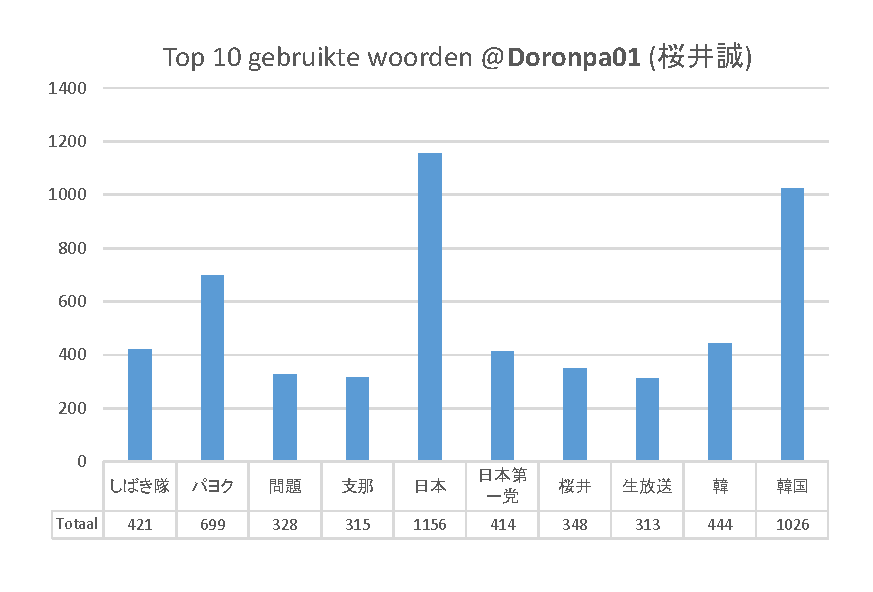
\includegraphics[width=.8\textwidth]{images/frequency.pdf}
    \centering\caption{Grafiek van de top tien meest gebruikte woorden uit de verworven Twittergegevens van Sakurai als corpus.}
\end{figure}

\begin{figure}
  \centering
    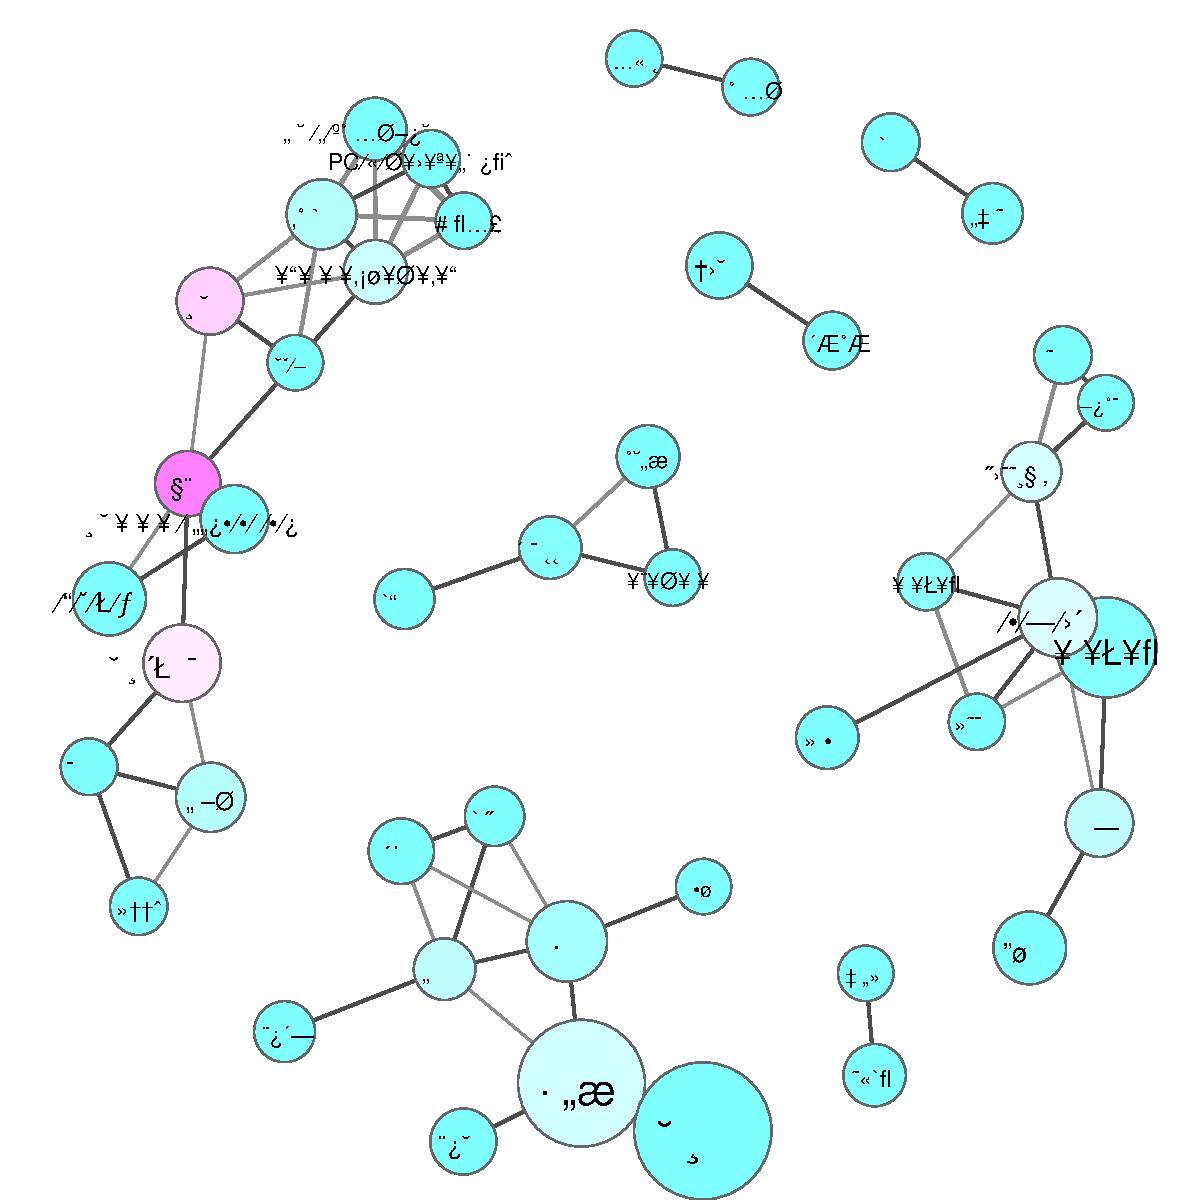
\includegraphics{images/co-occurance_network.pdf}
    \centering\caption{Co-occurrence netwerk van termen uit het Sakurai Twittercorpus met een hoge frequentie.}
\end{figure}

Als verwacht sluiten Sakurai's voorname politieke standpunten aan bij
die van de net rechtse stem als gedefinieerd in deel twee. Ook
terugblikkend naar \textbf{Tabel 1.2} lijken Sakurai's voorname
politieke standpunten aansluiting te vinden bij nativisme en
revisionisme als \emph{thick-centred} ideologieën. Historische problemen
worden gebagatelliseerd, en in een nulsomspel worden de rechten die
gegund worden aan minderheden gezien als een verlies van rechten voor
`de Japanner' (wat in deze context gezien kan worden als `leeg omhulsel'
of \emph{empty signifier}). Daaruit volgt een antagonisering van
minderheden, politieke entiteiten als de DPJ, en instituten als
massamedia. Sakurai, als nieuwe politieke speler en invloedrijke
\emph{netizen}, representeert aldus de `volkswil' van de net rechtse
beweging om tegen die anti-Japanse bewegingen te strijden, en kan zo
volgens de definitie in het eerste deel geclassificeerd worden als
populist. Daarboven maakt hij niet enkel sterk gebruik van
computerondersteunde communicatie om zijn ideologieën te propageren,
maar lijken die zelf deels te zijn gevormd uit het
\emph{netizen}-discours.

In analogie naar \textbf{Tabel 1.3} en de idee van een
internetdemocratie, blijft steun buiten de digitale regionen echter
relatief gering. Deelnames aan protestacties door de Zaitokukai blijven
veeleer beperkt tot internetdiscussies en het bekijken van
video-opnames. Politieke steun leidde in gouverneursverkiezingen van
2016 in Tokio tot een vijfde plaats als nieuwkomer uit 21 deelnemers,
maar dan nog betreft het slechts 1.74\% van het totaal aantal stemmen.
Het wordt afwachten naar de verkiezingen van juni 2017 om enige
mogelijke groei van Sakurai's Japan First Party waar te nemen en om echt
van een verschuiving op het Japanse politieke landschap te spreken.

\newpage

\section{Conclusie en Verder
Onderzoek}\label{conclusie-en-verder-onderzoek}

De notie van `digitaal populisme' is er een die nood heeft aan verdere
theoretische conceptualisatie, wat vermoeilijkt wordt door de fluïditeit
van de term `populisme' zelf. In een poging tot verdere theoretische
uitwerking van `digitaal populisme' voerde deze paper een sociale
identiteitsbenadering van het te mobiliseren electoraat of
\emph{heartland}, in dit geval de Japanse rechtse internetbeweging. De
synergie tussen demand-side kenmerken van populisme die leiden tot een
identiteitscrisis, en supply-side kenmerken als internet-democratie,
creëert een spiraal van nationalisme waaruit populisten kunnen ontstaan
of waarop ze kunnen inspelen. Enerzijds wordt, mede door het internet,
een latente visie van buitenlandse elementen als een dreigende `Ander'
naar boven gebracht en discursief in stand gehouden, anderzijds werkt
internetanonimiteit ook een versterkende band van \emph{netizens} in de
hand. Rumi (\protect\hyperlink{ref-rumiux5fkoreansux5f2011}{2011})
argumenteerde zo dat de ideologieën van net rechtsen niet onmiddellijk
gerelateerd hoeven te zijn aan economische redenen maar dat een
identiteit als iemand uit de net rechtse beweging discursief wordt
gecreëerd door middel van anonieme fora als 2channel.

Deze bachelorpaper dient voornamelijk tot het aantonen van enige
correlatie tussen internetcommunicatie en de groei aan populisten, met
mogelijke verschuivingen in het politieke landschap als gevolg. Stemmen
als Funabashi (\protect\hyperlink{ref-funabashiux5fjapanux5f2017}{2017})
stellen dat een rechtspopulisme als ervaren in West-Europa en de
Verenigde Staten heeft gefaald in Japan, maar een dergelijke stelling
lijkt echter te kort door te bocht. Het opentrekken van het Japans
politiek systeem en een sterke groei aan massamedia heeft tot een aantal
extreemrechtse grassrootsbewegingen en politieke partijen met
populistische ideologieën geleid. Individueel bekeken hebben die geen
sterke impact op het politiek landschap, maar als geheel lijken ze wel
een zekere trend in politiek denken te vormen. Als case-study spitste
deze paper zich toe op Sakurai Makoto, een spilfiguur binnen de net
rechtse beweging wiens ideologieën geboren lijken te zijn uit de het
\emph{netizens}-discours maar ook aan alle kenmerken van de opgestelde
definitie van populisme voldoen. Dat omdat hij bekend staat als net
rechtse internetpersonaliteit, en oprichter van beide
ultranationalistische volksbeweging Zaitokukai en de politieke Japan
First Party. Om Sakurai empirisch te bewijzen als iemand met
populistische ideologieën werd er een frequentieanalyse gemaakt over een
substantiële portie van zijn Twitter-activiteit. Daaruit vertrekkend kan
Sakurai's populisme, niet ongelijk aan dat in West-Europa en de
Verenigde Staten, als nativistisch en reactionair beschreven worden,
eerder als een neoliberaal populisme.

Populisme in Japan blijft een relatief nieuw studiegebied. Japanse
politicologen hebben al eerder gepoogd om het Japans populisme in kaart
te brengen met een vernieuwde focus op het belang van media, maar de rol
van het internet in het politieke landschap vanaf 2000 tot vandaag
blijft zo goed als onbesproken. De jaartallen 2002 en 2011 worden echter
zowel in de lectuur als in het mainstream discours beschouwd als
keerpunt in de perceptie van mainstream media en groei van de net
rechtse stem. Het zal een uitdaging zijn dat empirisch te bewijzen. Een
optie daarvoor is het verder utiliseren van de relatief nieuwe
mogelijkheden die sociale netwerkanalyse (SNA) biedt aan sociologisch
onderzoek. Een eerste stap zou kunnen zijn om massaal gegevens van
sociale netwerkdiensten te verzamelen over een periode vóór en ná 2011
en, via een frequentie-analyse van aan net rechts verbonden
terminologie, een (potentiële) relatieve stijging aan te tonen.

Verder kan het thema ook verder opengegooid worden door het
internetgebruik van de andere kant van het politieke spectrum te
bekijken. De linkse internetbeweging wordt vaak aangeduid met termen als
\emph{netto-sayoku} (ネット左翼) of pejoratief \emph{netopayo}
(ネトぱよ). Die internetbeweging wordt geassocieerd met linkse
volksbewegingen als C.R.A.C. en SealDs, en aanhangers van de CPJ en DPJ.
Tenslotte loont het de moeite om digitaal populisme in China en
Zuid-Korea te onderzoeken en enige synergie met die bewegingen in Japan
in kaart te brengen. Het Koreaanse anonieme forum ILBE (일베) heeft
bijvoorbeeld veel overeenkomstige kenmerken met 2channel en wordt
geassocieerd met uiterst rechtse, patriottische ideologieën en
anti-buitenlandse meningen (Kim
\protect\hyperlink{ref-kimux5filbeux5f2013}{2013}; Lew, Cho, en Park
\protect\hyperlink{ref-lewux5fpoliticizationux5f2014}{2014}). De vraag
kan dan gesteld worden of dat digitaal populisme in die drie landen
verdere dispersie van extreem-nationalisme, escalatie van conflicten en
wantrouwen jegens elkaar in gang zet.

\newpage

\appendix

\section{Bijlagen}\label{bijlagen}

\subsection{Methodologie}\label{methodologie}

(Kwantitatieve) tekstanalyse van Japanse teksten wordt vermoeilijkt door
de structuur van de Japanse taal (Catalinac
\protect\hyperlink{ref-catalinacux5fquantitativeux5f2014}{2014}). Om
tekstanalyse uit te voeren is er nood aan software die Japanse teksten
morfologisch kan analyseren. Daarin is de keuze relatief beperkt:
historisch wordt vooral verwezen naar JUMAN\footnote{\url{http://nlp.ist.i.kyoto-u.ac.jp/?JUMAN}}
en ChaSen,\footnote{\url{http://chasen.naist.jp/hiki/ChaSen/}} maar deze
paper maakt gebruik van de \emph{open-source}-applicatie MeCab\footnote{\url{http://taku910.github.io/mecab/}}
die verderbouwt op ChaSen en zowel sneller werkt als meer betrouwbare
resultaten oplevert (Den e.a.
\protect\hyperlink{ref-denux5fproperux5f2008}{2008}). Vervolgens
gebruikt deze paper voor tekstanalyse zelf de
\emph{open-source}-applicatie KH Coder.\footnote{Ontwikkeld door Higuchi
  Kōichi (樋口耕一), associate professor of Social Sciences aan
  Ritsumeikan Universiteit in Kioto. Beschikbaar op
  \url{http://khc.sourceforge.net/en/}. Maakt achterliggend gebruikt van
  de \textbf{R} programmeeromgeving, gericht op statistisch onderzoek en
  data-analyse.} Zoals eerder aangegeven bestaat het corpus van de
tekstanalyse uit data gehaald uit Twitter, een proces dat in het
volgende deel wordt beschreven.

\subsubsection{Twitter Datamining}\label{twitter-datamining}

De achterliggende software van Twitter is op dergelijke wijze gebouwd
dat het gebruik daarvan, en aldus de mogelijkheid tot dataverwerving, op
relatief eenvoudige wijze kan worden uitgevoerd. Die software is, uit
commerciële redenen, zo opgebouwd om aangesproken te kunnen worden door
andere software en dus om interactiviteit tussen (web)applicaties te
verhogen. Grote commerciële bedrijven gebruiken die mogelijkheden vooral
om patronen en verbanden te leggen in grote hoeveelheden aan data en op
die manier economische strategieën op te stellen of om vooruitzichten te
creëren.

Het analyseren van data gehaald uit sociale netwerken kent ook een
opmars in academisch onderzoek. De enorme hoeveelheid aan openbaar
beschikbare data leunt daar daar goed bij aan: sinds 2013 worden elke
dag worden door 238 miljoen actieve gebruikers ongeveer 500 miljoen
Tweets verzonden. Tweets bevatten naast de tekstuele inhoud
meta-informatie als demografische gegevens van de zender, het aantal
keer dat het bericht gedeeld werd, enzovoort. Het gebruik daarvan is
echter nog beperkt door de limitaties die Twitter op de software
plaatst. Berichten zijn in principe openbaar maar enkel een deel daarvan
is gratis beschikbaar. Zowel toegang tot historische data als tot wat
Twitter de \emph{firehose} noemt (toegang tot 100\% van de berichten die
\emph{real-time} geplaatst worden) vereist licenties met
\emph{resellers} als Gnip die ver boven het budget liggen van een
gemiddelde academicus.

Indien volledigheid van data, of nauwkeurigheid over de periode van het
aantal berichten niet van belang zijn voor het onderzoek daarop
uitgevoerd, kan de software gratis aangesproken. Wel zijn er enige
limitaties: het ophalen van de berichten (met de Streaming API) die
\emph{real-time} geplaatst worden kan beperkt worden tot 1\% van het
totaal, en ook het historisch ophalen met de Search API wordt beperkt in
aantal (3200 berichten per individu) of periode (maximaal 7 dagen terug
voor opzoekingen op kernwoorden).

\subsubsection{Dataset van Makato
Sakurai}\label{dataset-van-makato-sakurai}

De dataset die gebruikt wordt in de kwantitatieve inhoudsanalyse bevat
de laatste 3200 publieke berichten en \emph{retweets} geplaatst door
Sakurai Makoto op Twitter-account \textbf{@Doronpa01}
(\url{https://twitter.com/doronpa01}) en werd samengesteld om 4/04/2017
14:00. De dataset werd samengesteld door de Twitter (Search) API
recursief aan te spreken met Python tot elk tweet-bestand verzameld werd
in een JSON-bestand. De limitatie van 3200 berichten werd opgelegd door
de API van Twitter -- naast het webscrapen van elk individueel bericht
(wat een hoop moeilijkheden oplevert door de opbouw van het platform
zelf, berichten worden gegenereerd door JavaScript) is er nog geen
mogelijkheid om die te omzeilen. Het Python-script (licht gewijzigd om
enige Twitter-identificatie weg te laten) is online als digitale bijlage
te raadplegen op
\url{https://github.com/steviepoppe/bachelor_paper/tree/master/python}.

De dataset werd vervolgens opgekuist met \textbf{Open Refine} door voor
deze paper overbodige meta-informatie te verwijderen. Voor de
tekstanalyse werd enkel de tekst van het Twitterobject zelf gebruikt,
met omissie van enige bijlagen en externe URL's.

\subsubsection{Frequentieanalyse}\label{frequentieanalyse}

De frequentieanalyse als weergegeven in \textbf{figuur 7} en
\textbf{figuur 8} werd uitgevoerd met KH Coder, gebruikmakend van MeCab
om de tekst morfologisch te analyseren. Een bijkomende lijst werd
opgesteld om samenstellingen, afkortingen en vaak voorkomende elementen
(zoals \emph{kōdōsuru hoshu undō} 行動する保守運動 en \emph{kitachō}
北鮮) niet uit elkaar te trekken. Die lijst, alsook de volledige
frequentieanalyse als CSV zijn beschikbaar als digitale bijlage op
\url{https://github.com/steviepoppe/bachelor_paper/tree/master/textanalysis}.

Vervolgens werd er een verbindingsmatrix van kernwoorden uit de
frequentieanalyse opgesteld, gebaseerd op het gelijktijdig optreden
daarvan. Die matrix werd in KH Coder geplot aan de hand van het
Fruchterman-Reingold layout-algoritme. Kleuren per node worden berekend
aan de hand van betweenness-centraliteit: hoe sterker de kleur hoe
korter het pad tussen de termen.

Ten slotte werd door middel van \textbf{Tableau} een interactieve
visuele weergave samengesteld van de gebruikte dataset. Dat werd gedaan
door enerzijds de oorspronkelijke, volledige Tweet-dataset en anderzijds
de daarvan afgeleide frequentielijst (gelimiteerd tot 150 kernwoorden)
te gebruiken. Bezoekers kunnen de Twitterdata sorteren en filteren op
kernwoorden, eigen zoekacties, een tijdspanne, succes (op basis van
\emph{retweets} en \emph{favorites}) of een combinatie daarvan. Het
resultaat valt te raadplegen op \url{https://steviepoppe.net/bachelor/}.

\newpage

\section*{Referenties}\addcontentsline{toc}{section}{Referenties}

\setlength{\parindent}{-0.2in} \setlength{\leftskip}{0.2in}
\setlength{\parskip}{0em} \noindent

Als standaard in de sociale wetenschappen hanteert dit document
\textbf{Chicago B} (`auteur-jaarsysteem') als verwijzingssysteem.

\vspace{4mm}

\setlength{\parskip}{0em} \footnotesize

\hypertarget{refs}{}
\hypertarget{ref-2021ux5fsummerux5fhashimotoux5f2014}{}
2021 summer. 2014. 「橋下徹vs在特会・桜井誠 【全】10/20」 (\emph{“Hashimoto Tōru vs Zaitokukai ・Sakurai Makoto [zen] 10/20”}, Ned: Hashimoto Tōru VS Zaitokukai  en Sakurai Makoto [Volledig] 10/20). YouTube video, 07:59. Gepubliceerd op [20 okt. 2014]. \url{https://youtu.be/ACRxHAC-tyg} (Geraadpleegd op 17 april 2017).

\hypertarget{ref-2ch.netux5fsuzumeux5f2017}{}
2ch.net. 2017. 「すずめ」 \emph{(“suzume”)}. \emph{2ch.net}. \url{http://stats.2ch.net/suzume.cgi?yes} (Geraadpleegd op 16 april 2017).

\hypertarget{ref-abtsux5fpopulismux5f2007}{}
Abts, K., en S. Rummens. 2007. “Populism versus Democracy”. 
\emph{Political Studies} 55 (2): 405--24.
doi:\href{https://doi.org/10.1111/j.1467-9248.2007.00657.x}{10.1111/j.1467-9248.2007.00657.x}.

\hypertarget{ref-alexa.comux5fnicovideo.jpux5f2017}{}
Alexa.com. 2017a. “Nicovideo.jp Traffic, Demographics and Competitors - Alexa”. \emph{alexa.com}. \url{http://www.alexa.com/siteinfo/nicovideo.jp} (Geraadpleegd op 15 april 2017).

\hypertarget{ref-alexa.comux5ftopux5f2017}{}
Alexa.com. 2017b. “Top Sites in Japan - Alexa”.  \emph{alexa.com}. \url{http://www.alexa.com/topsites/countries/JP} (Geraadpleegd op 15 april 2017).

\hypertarget{ref-alvaresux5fpopulismux5f2016}{}
Alvares, Claudia, en Peter Dahlgren. 2016. “Populism, extremism and
media: Mapping an uncertain terrain.”  \emph{European Journal of
Communication} 31 (1): 46--57.

\hypertarget{ref-andersonux5fimaginedux5f2006}{}
Anderson, Benedict R. O'G. 2006. \emph{Imagined communities: Reflections
on the origin and spread of nationalism}. Rev. ed. London ; New York:
Verso.

\hypertarget{ref-appaduraiux5fmodernityux5f1996}{}
Appadurai, Arjun. 1996. \emph{Modernity at large: Cultural dimensions of
globalization}. Public worlds, v. 1. Minneapolis, Minn: University of
Minnesota Press.

\hypertarget{ref-baleux5fthrownux5f2011}{}
Bale, Tim, Stijn Van Kessel, en Paul Taggart. 2011. “Thrown around with
abandon? Popular understandings of populism as conveyed by the print
media: A UK case study.”  \emph{Acta Politica; Basingstoke} 46 (2):
111--31.
doi:\href{https://doi.org/10.1057/ap.2011.3}{10.1057/ap.2011.3}.

\hypertarget{ref-betzux5ftwoux5f1993}{}
Betz, Hans-Georg. 1993. “The two faces of radical right-wing populism in
Western Europe.”  \emph{The Review of Politics} 55 (04): 663--86.

\hypertarget{ref-bimberux5finternetux5f1998}{}
Bimber, Bruce. 1998. “The Internet and Political Transformation:
Populism, Community, and Accelerated Pluralism.” \emph{Polity} 31 (1):
133--60. doi:\href{https://doi.org/10.2307/3235370}{10.2307/3235370}.

\hypertarget{ref-catalinacux5fquantitativeux5f2014}{}
Catalinac, Amy. 2014. “Quantitative Text Analysis with Asian Languages:
Some Problems and Solutions.”  \emph{Polimetrics} 1 (1): 14--17.

\hypertarget{ref-denux5fproperux5f2008}{}
Den, Yasuharu, Junpei Nakamura, Toshinobu Ogiso, en Hideki Ogura. 2008.
“A Proper Approach to Japanese Morphological Analysis: Dictionary, Model,
and Evaluation.”  In \emph{LREC}.

\hypertarget{ref-engesserux5fpopulismux5f2017}{}
Engesser, Sven, Nicole Ernst, Frank Esser, en Florin Büchel. 2017.
“Populism and social media: How politicians spread a fragmented ideology.”  
\emph{Information, Communication \& Society} 20 (8): 1109--26.
doi:\href{https://doi.org/10.1080/1369118X.2016.1207697}{10.1080/1369118X.2016.1207697}.

\hypertarget{ref-facklerux5fnewux5f2010}{}
Fackler, Martin. 2010. “New Dissent in Japan Is Loudly Anti-Foreign”.  \emph{The New York Times}, augustus 28. \url{http://www.nytimes.com/2010/08/29/world/asia/29japan.html} (Geraadpleegd op 10 april 2016).

\hypertarget{ref-funabashiux5fjapanux5f2017}{}
Funabashi, Yoichi. 2017. “Japan, Where Populism Fails”.  \emph{The New York Times}, februari 8. \url{https://www.nytimes.com/2017/02/08/opinion/japan-where-populism-fails.html} (Geraadpleegd op 5 april 2017).

\hypertarget{ref-furuyaux5fcanux5f2016}{}
Furuya, Tsunehira. 2016. “Can Laws Control Japan’s Hate Epidemic?”.  \emph{nippon.com}. \url{http://www.nippon.com/en/currents/d00224/} (Geraadpleegd op 25 mei 2017).

\hypertarget{ref-gottliebux5fjapaneseux5f2003}{}
Gottlieb, Nanette, en Mark J. McLelland, red. 2003. \emph{Japanese
cybercultures}. Asia's transformations. London ; New York: Routledge.

\hypertarget{ref-hackux5fsubcultureux5f2016}{}
Hack, Brett. 2016. “Subculture as social knowledge: A hopeful reading of
otaku culture.”  \emph{Contemporary Japan} 28 (1).
doi:\href{https://doi.org/10.1515/cj-2016-0003}{10.1515/cj-2016-0003}.

\hypertarget{ref-haleux5fpoliticalux5f2016}{}
Hale, Scott, Peter John, Helen Margetts, en Taha Yasseri. 2016.
Political turbulence: How social media shape collective action.

\hypertarget{ref-higuchiux5fjapansux5f2014}{}
Higuchi, Naoto. 2014a. “Japan's Far Right in East Asian Geopolitics: The
Anatomy of New Xenophobic Movements.”  \emph{Social Science Research,
University of Tokushima} 28: 163--83.

\hypertarget{ref-higuchiux5fned:ux5f2014}{}
Higuchi, Naoto (樋口直人). 2014b. 『日本型排外主義 : 在特会・外国人参政権・東アジア地政学』 (\emph{Nihon-gata haigai shugi: Zaitokukai, gaikokujin sanseiken, Higashi Ajia chiseigaku}, Ned: \emph{Het Japans Model van Xenofobisch Exclusionisme: Zaitokukai, Kiesrecht voor Buitenlanders en Oost-Aziatische geopolitiek}). Nagoya: Nagoya Daigaku Shuppankai (名古屋大学出版会).

\hypertarget{ref-hollihanux5fdisputeux5f2014}{}
Hollihan, Thomas A. 2014. \emph{The dispute over the Diaoyu/Senkaku
Islands: How media narratives shape public opinion and challenge the
global order}. Palgrave macmillan series in international political
communication.

\hypertarget{ref-horiuchiux5fpublicux5f2014}{}
Horiuchi, Toru. 2014. “Public Opinion in Japan and the Nationalization of
the Senkaku Islands.”  \emph{East Asia} 31 (1): 23--47.
doi:\href{https://doi.org/10.1007/s12140-014-9202-6}{10.1007/s12140-014-9202-6}.

\hypertarget{ref-hosyuux5fzaitokukaiux5f2013}{}
HoSyu. 2013.  「在特会会長、しばき隊ら逮捕の件 アサヒの報道は・・・」 \emph{(“Zaitokukai kaichō, shiba ki-tai-ra taiho no kudan Asahi no hōdō wa”)}. Niconico Video, 0:59. Gepubliceerd op [16 jun. 2013]. \url{http://www.nicovideo.jp/watch/sm21136388} (Geraadpleegd op 16 april 2017).

\hypertarget{ref-theux5fchosunux5filboux5fjapaneseux5f2011}{}
The Chosun Ilbo. 2011. “Japanese March Against Korean Soap Operas”, chosun.com, augustus 22.\url{ http://english.chosun.com/site/data/html_dir/2011/08/22/2011082200679.html} (Geraadpleegd op 12 april 2016).

\hypertarget{ref-theux5fdongaux5filboux5fjapansux5f2011}{}
The Dong-a Ilbo. 2011. “Japan’s right-wing groups hold rallies vs. Korean pop culture”, donga.com, augustus 9. \url{http://english.donga.com/List/3/all/26/401888/1} (Geraadpleegd op 12 april 2016).

\hypertarget{ref-itagakiux5fanatomyux5f2015}{}
Itagaki, Ryuta. 2015. “The Anatomy of Korea-phobia in Japan.” 
\emph{Japanese Studies} 35 (1): 49--66.
doi:\href{https://doi.org/10.1080/10371397.2015.1007496}{10.1080/10371397.2015.1007496}.

\hypertarget{ref-itoux5ffandomux5f2012}{}
Itō, Mizuko, Daisuke Okabe, en Izumi Tsuji. 2012. \emph{Fandom unbound:
Otaku culture in a connected world}.

\hypertarget{ref-jooeunux5fgreatux5f2011}{}
Jooeun, Noh. 2011. “The Great Kantō Earthquake, the Korean Massacre and
its Aftermath: The Responsibility of the Japanese Government and People
\textbar{} Harvard-Yenching Institute.” 
\url{https://www.harvard-yenching.org/the-great-kanto-earthquake} (Geraadpleegd op 6 mei 2017).

\hypertarget{ref-katayamaux5f2-channelux5f2007}{}
Katayama, Lisa. 2007. “2-Channel Gives Japan’s Famously Quiet People a Mighty Voice”. \emph{WIRED}, april 19. \url{http://archive.wired.com/culture/lifestyle/news/2007/04/2channel} (Geraadpleegd op 11 april 2017).

\hypertarget{ref-kieslerux5fsocialux5f1984}{}
Kiesler, Sara, Jane Siegel, en Timothy W. McGuire. 1984. “Social
psychological aspects of computer-mediated communication.”  \emph{American
Psychologist} 39 (10): 1123--34.
doi:\href{https://doi.org/10.1037/0003-066X.39.10.1123}{10.1037/0003-066X.39.10.1123}.

\hypertarget{ref-kimux5filbeux5f2013}{}
Kim, Jong-mok. 2013. “Ilbe and Japan’s Net Right: Resemblances Triggered by the Little Hatred and Despair in the Hearts of Ordinary People”. \emph{The Kyunghyang Shinmun}, juni 4.  \url{http://english.khan.co.kr/khan_art_view.html?artid=201306041754247&code=710100l} (Geraadpleegd op 20 mei 2017).

\hypertarget{ref-kimux5fdigitalux5f2009}{}
Kim, Youngmi. 2009. “Digital Populism in South Korea? Internet Culture
and the Trouble with Direct Participation.”  \emph{On Korea: Academic
Papers Series} 3 (8): 1--6.

\hypertarget{ref-koboriux5fpopulismux5f2013}{}
Kobori, Masahiro. 2013. “Populism as Rhetorical Politics in Britain and
Japan : 'Devil take the hindmost'.” \emph{Ritsumeikan law review}, juli,
107--22.

\hypertarget{ref-kramerux5fmediaux5f2014}{}
Krämer, Benjamin. 2014. “Media Populism: A Conceptual Clarification and
Some Theses on its Effects: Media Populism.” \emph{Communication Theory}
24 (1): 42--60. 
doi:\href{https://doi.org/10.1111/comt.12029}{10.1111/comt.12029}.

\hypertarget{ref-laclauux5fpopulistux5f2005}{}
Laclau, Ernesto. 2005. \emph{On populist reason}. London ; New York:
Verso.

\hypertarget{ref-leaux5fcomputer-mediatedux5f1991}{}
Lea, Martin, en Russell Spears. 1991. “Computer-mediated communication,
de-individuation and group decision-making.”  \emph{International Journal
of Man-Machine Studies} 34 (2): 283--301.
doi:\href{https://doi.org/10.1016/0020-7373(91)90045-9}{10.1016/0020-7373(91)90045-9}.

\hypertarget{ref-leaux5fsocialux5f1992}{}
Lea, Martin, red. 1992. “Social influence and the influence of the
'social' in computer-mediated communication.”  In \emph{Contexts of
computer-mediated communication}, pp. 30--65. New York: Harvester
Wheatsheaf.

\hypertarget{ref-leeux5fdeindividuationux5f2007}{}
Lee, Eun-Ju. 2007. “Deindividuation Effects on Group Polarization in
Computer-Mediated Communication: The Role of Group Identification,
Public-Self-Awareness, and Perceived Argument Quality.” \emph{Journal of
Communication} 57 (2): 385--403.
doi:\href{https://doi.org/10.1111/j.1460-2466.2007.00348.x}{10.1111/j.1460-2466.2007.00348.x}.

\hypertarget{ref-lewux5fpoliticizationux5f2014}{}
Lew, Seok-jin, Hee-jung Cho, en Seol-ah Park. 2014. “Politicization of
Online Neo-nationalism in Korea, China and Japan.”  \emph{Institute of
Korean Political Studies, Seoul National University} 22 (13): 62--75.

\hypertarget{ref-lieux5fzainichiux5f2008}{}
Lie, John. 2008. \emph{Zainichi (Koreans in Japan): Diasporic
nationalism and postcolonial identity}. Global, area, and international
archive. Berkeley: University of California Press.

\hypertarget{ref-lindgrenux5fdevelopingux5f2015}{}
Lindgren, Petter Y. 2015. “Developing Japanese Populism Research through
Readings Of European Populist Radical Right Studies: Populism As An
Ideological Concept, Classifications Of Politicians And Explanations For
Political Success.” \emph{Japanese Journal of Political Science} 16 (04):
574--92.
doi:\href{https://doi.org/10.1017/S1468109915000328}{10.1017/S1468109915000328}.

\hypertarget{ref-maslowux5fnationalismux5f2011-1}{}
Maslow, Sebastian. 2011. “Nationalism 2.0 in Japan (http://www.2ch.net/):
Electronic Media Reviews.”  \emph{Asian Politics \& Policy} 3 (2):
307--10.
doi:\href{https://doi.org/10.1111/j.1943-0787.2011.01265.x}{10.1111/j.1943-0787.2011.01265.x}.

\hypertarget{ref-matsumuraux5fdynamismux5f2005}{}
Matsumura, Naohiro, Asako Miura, Yasufumi Shibanai, Yukio Ohsawa, en
Toyoaki Nishida. 2005. “The dynamism of 2channel.”  \emph{AI \& SOCIETY} 19
(1): 84--92.
doi:\href{https://doi.org/10.1007/s00146-004-0302-5}{10.1007/s00146-004-0302-5}.

\hypertarget{ref-matsutaniux5fwakamonoux5f2009}{}
Matsutani, Mitsuru (松谷満). 2009. 「若者におけるポピュリズムの支持基盤: ミリュー・アプローチによる実証的検討」 (\emph{“Wakamono ni okeru popyurizumu no shiji kiban: Miryū apu rōchi ni yoru jisshō-teki kentō”}, Ned: Draagvlak van het Populisme Onder de Jeugd: een Empirisch Onderzoek van Milieu Benadering).  『茨城大学地域総合研究所年報』(\emph{Ibarakidaigaku chiiki sōgōkenkyūsho nenpō}, Ibaraki Universiteit Regionale Onderzoeksinstituut Jaarverslag), 42 (maart): 41–59.

\hypertarget{ref-matsutaniux5fnihon-gataux5f2010}{}
Matsutani, Mitsuru (松谷満). 2010. 「日本型ポピュリズムの論理と心情--大都市無党派層の実証研究」 (\emph{“Nihon-gata popyurizumu no ronri to shinjō -- daitoshi mutōha-sō no jisshō kenkyū”}, Ned: De Logica en Emotie van de Japanse Stijl van Populisme: een Empirisch Onderzoek naar Onafhankelijke Kiezers in de Japanse Metropolen. \emph{KAKEN}. \url{https://kaken.nii.ac.jp/grant/KAKENHI-PROJECT-21730428/} (Geraadpleegd op 8 april 2017).

\hypertarget{ref-matsutaniux5fpopyurizumuux5f2011}{}
Matsutani, Mitsuru (松谷満). 2011. 「ポピュリズムの台頭とその源泉 (特集 政党への幻滅の中の地方選--何が台頭するか)」 (\emph{Popyurizumu no taitō to sono gensen (tokushū seitō e no genmetsu no naka no chihō-sen -- nani ga taitō suru ka)”}, Ned: De Logica en Emotie van de Japanse Stijl van Populisme: een Empirisch Onderzoek naar Onafhankelijke Kiezers in de Japanse Metropolen).   『世界 』(\emph{sekai}, Wereld), nr. 815 (april): 133–41.

\hypertarget{ref-mieux5fxenophobiaux5f2013}{}
Mie, Ayako. 2013. “Xenophobia Finds Fertile Soil in Web Anonymity”. \emph{The Japan Times Online}, januari 8. \url{http://www.japantimes.co.jp/news/2013/01/08/reference/xenophobia-finds-fertile-soil-in-web-anonymity/} (Geraadpleegd op 31 maart 2016).

\hypertarget{ref-izumiux5fmihashiux5fconfessionsux5f2015}{}
Mihashi, Izumi. 2015. “Confessions of Former Japanese ‘Netto-Uyoku’ Internet Racists \(\cdot\) Global Voices”. \emph{Global Voices}. \url{https://globalvoices.org/2015/03/23/confessions-of-former-japanese-netto-uyo-internet-racists/} (Geraadpleegd op 19 maart 2016).

\hypertarget{ref-morris-suzukiux5fre-imaginingux5f2011}{}
Morris-Suzuki, Tessa. 2011. “Re-Imagining Japan-North Korea Relations.”
\emph{The Japan Institute}.

\hypertarget{ref-morris-suzukiux5ffreedomux5f2013}{}
Morris-Suzuki, Tessa. 2013. “Freedom of Hate Speech; Abe Shinzo and Japan’s Public Sphere”, The asia-pacific journal, Volume 11, Issue 8, Number 1
(februari).

\hypertarget{ref-morris-suzukiux5fbeyondux5f2015}{}
Morris-Suzuki, Tessa. 2015.  “Beyond Racism: Semi-Citizenship and Marginality in Modern Japan” \emph{Japanese Studies} 35 (1): 67--84.
doi:\href{https://doi.org/10.1080/10371397.2015.1014469}{10.1080/10371397.2015.1014469}.

\hypertarget{ref-muddeux5fpopulistux5f2007}{}
Mudde, Cas. 2007. \emph{Populist Radical Right Parties in Europe}.
Cambridge, UK ; New York: Cambridge University Press.

\hypertarget{ref-muddeux5foxfordux5f2013}{}
Mudde, Cas. 2013. \emph{The Oxford handbook of political ideologies}.
Bewerkt door Michael Freeden, Lyman Tower Sargent, en Marc Stears. First
edition. Oxford handbooks in politics \& international relations.
Oxford, United Kingdom: Oxford University Press.

\hypertarget{ref-muraiux5fnetux5f2012}{}
Murai, Shusuke. 2012. “Net Uyoku: A Global Confrontation of Radical
Nationalism in the Borderless World.” \emph{The Asian Conference on Media
and Mass Communication}, MediAsia.

\hypertarget{ref-mutsuoux5ftoiux5fhigashinihonux5f2011}{}
mutsuo_toi. 2011. 「東日本大震災の直後に広がった人種差別と「レイプ多発」というデマ」\emph{(“Higashinihon daishinsai no chokugo ni hirogatta hito shusabetsu to `reipu tahatsu’ to iu dema”, Ned: Het Racisme dat vlak na de Aardbeving in 2011 Sterk verspreidde en Geruchten over Frequente Verkrachtingen.)}. \emph{Togetter.com} (blog). november 3. \url{https://togetter.com/li/110490} (Geraadpleegd op 6 mei 2017).

\hypertarget{ref-nanakoux5f1892ux5fzainichikankokujinux5f2014}{}
nanako_1892. 2014. 「在日韓国人が東北震災で亡くなった日本人の戸籍を利用している。いわゆる「背のり」だ。」 (\emph{(“Zainichikankokujin ga Tōhoku shinsai de nakunatta nihonjin no koseki o riyō shite iru. Iwayuru `hainori’ da.”}, Ned: Zainichi Koreanen gebruiken het familieregister van Japanners die overleden zijn na de Tohoku Aardbeving. Dat is met andere woorden "hainori".). \emph{Yahoo! Japan} (blog). januari 24. \url{https://detail.chiebukuro.yahoo.co.jp/qa/question_detail/q14119924654} (Geraadpleegd op 6 mei 2017).

\hypertarget{ref-nikkeiux5fnewsux5fdemo-meguriux5f2013}{}
Nikkei News. 2013. 「デモ巡り乱闘、男女8人を暴行容疑で逮捕 東京・新宿」 (\emph{( “Demo-meguri rantō, danjo 8-ri o bōkō yōgi de taiho Tōkyō Shinjuku”} Ned: Uitgebroken Gevechten tijdens een Demonstratie, 8 Mensen Gearresteerd op Verdenking van Geweld in Tokio en Shinjuku). Nikkei.com, juni 17. \url{http://www.nikkei.com/article/DGXNASDG1601P_W3A610C1CC1000/} (Geraadpleegd op 15 april 2017).

\hypertarget{ref-sankeiux5fnewsux5ftokyochiji-senux5f2016}{}
Sankei News. 2016a. 「 【東京都知事選】「都内在住外国人への生活保護費支給打ち切り、受給者は日本国民限定」 在特会の桜井誠前会長が7つの公約」 (\emph{( “tonai zaijū gaikokujin e no seikatsu hogo-hi shikyū uchikiri, jukyū-sha wa nihonkokumin gentei’ zaitokkai no sakurai makoto zen kaichō ga nanatsu no kōyaku”} Ned: [Tokyo Gouverneursverkiezing] Stop het Betalen van Welzijnskosten aan Buitenlandse Bewoners in Tokio, en Beperk Begunstigden tot Enkel Japanners" De 7 Beloftes van ex-Zaitokukai Voorzitter Sakurai Makoto). Sankei.com, juni 30. \url{http://www.sankei.com/politics/news/160629/plt1606290061-n1.html} (Geraadpleegd op 12 april 2017).

\hypertarget{ref-sankeiux5fnewsux5ftokyochiji-senux5f2016-1}{}
Sankei News. 2016b. 「【東京都知事選】桜井誠氏が激白!「間違ったことはしていない」「来年の都議選に10~20人立候補させます」」 (\emph{( “(Tōkyōto chiji-sen) sakurai makoto-shi ga gekihaku! `Machigatta koto wa shite inai’`rainen no togi-sen ni 10 ~ 20-jin rikkōho sasemasu’”} Ned: (Tokio Gouverneursverkiezingen) De Heer Makoto Sakurai Onthult! 'Ik Doe Geen Verkeerde Dingen', 'In de Tokio Grootstedelijke Verkiezingen Volgend jaar zal Ik 10-20 Personen Laten Deelnemen'). Sankei.com, juli 13. \url{http://www.sankei.com/premium/news/160713/prm1607130011-n1.html} (Geraadpleegd op 11 april 2017).

\hypertarget{ref-nicovideo.jpux5fpuremiamuux5f2015}{}
Nicovideo.jp. 2015. 「プレミアム会員数250万、総登録会員数5,000万を突破 - ニコニコ動画 開発者ブログ(新着情報)」\emph{(“Puremiamu kaiin sū 250 man, sō tōroku kaiin sū 5, 000 man o toppa - nikoniko dōga kaihatsu-sha burogu (shinchaku jōhō)”, Ned: Premium lidmaatschap 2,5 miljoen, totaal geregistreerde leden 50 miljoen, een doorbraak - Nico Nico Douga developers blog (Nieuws).)}. \emph{Nicovideo.jp} (blog). augustus 6. \url{http://blog.nicovideo.jp/2015/08/2505000.php} (Geraadpleegd op 15 april 2017).

\hypertarget{ref-ux5fheitosupiichiux5f2016}{}
Nikaido, Yuki. 2016. 「ヘイトスピーチ、3年半で1152件 政府が初の調査」 (\emph{( “Heitosupīchi, 3-nen han de 1152-ken seifu ga hatsu no chōsa: Asahishinbun dejitaru”} Ned: Aanzetten tot haat, op drie-en-een-half jaar 1152 incidenten, de eerste enquête van de overheid). 『朝日新聞』 (\emph{Asahi Shinbun}), juni 30. \url{http://www.asahi.com/articles/ASJ3X7WYZJ3XUUPI004.html} (Geraadpleegd op 31 april 2016).

\hypertarget{ref-ogiueux5fkenshoux5f2011}{}
Ogiue, Chiki (荻上チキ). 2011. 『検証 東日本大震災の流言・デマ』 (\emph{Kenshō Higashi Nihon Daishinsai no ryūgen, dema}, Ned: \emph{Ned: Geruchten na de 2011}). Tokio: Kōbunsha (光文社).

\hypertarget{ref-okazakiux5ftwitterux5f2012}{}
Okazaki, Akira (岡崎晃). 2012. Twitter Post. \emph{@okazaki\_akira}. 30 apr. 2012 - 17:02. \url{https://twitter.com/okazaki_akira/status/197113816344043523}.

\hypertarget{ref-osakiux5ffujiux5f2015}{}
Osaki, Tomohiro. 2015. “Fuji TV apologizes for subtitles inaccurately quoting South Koreans”. \emph{The Japan Times}, juni 29. \url{http://www.japantimes.co.jp.kuleuven.ezproxy.kuleuven.be/news/2015/06/29/national/social-issues/fuji-tv-apologizes-subtitles-inaccurately-quoting-south-koreans/} (Geraadpleegd op 12 april 2017).

\hypertarget{ref-ottux5fageux5f2017}{}
Ott, Brian L. 2017. “The age of Twitter: Donald J. Trump and the politics
of debasement.” \emph{Critical Studies in Media Communication} 34 (1):
59--68.
doi:\href{https://doi.org/10.1080/15295036.2016.1266686}{10.1080/15295036.2016.1266686}.

\hypertarget{ref-paelinckux5fpost-truthux5f2016}{}
Paelinck, Gianni. 2016. “'Post-truth' is woord van het jaar voor Oxford
Dictionaries”. \emph{deredactie.be}.
\url{http://deredactie.be/cm/vrtnieuws/buitenland/1.2820305} (Geraadpleegd op 18 april 2017).

\hypertarget{ref-japanux5ffirstux5fpartyux5fjapanux5f2016}{}
Japan First Party. 2016. 「日本第一党」 \emph{(“Nihon daiichi-tō”)}, \emph{japan-first.net}.\url{http://japan-first.net/policy.html} (Geraadpleegd op 16 april 2017).

\hypertarget{ref-penneyux5fracistsux5f2013}{}
Penney, Matthew. 2013. “``Racists Go Home!'', ``Go Crawl Back to the
Net!'' -Racism Protestors Confront the Zaitokuka”, The asia-pacific
journal, Issue 16 (april).

\hypertarget{ref-bbcux5fworldux5fserviceux5fpollux5f2014ux5f2014}{}
BBC World Service Poll. 2014. “2014 Country Rating Poll”. \url{http://www.globescan.com/images/images/pressreleases/bbc2014_country_ratings/2014_country_rating_poll_bbc_globescan.pdf} (Geraadpleegd op 6 mei 2017).

\hypertarget{ref-ricardoux5fbuettnerux5fsystematicux5f2016}{}
Ricardo Buettner. 2016. “A Systematic Literature Review of Twitter
Research from a Socio-Political Revolution Perspective.”
doi:\href{https://doi.org/10.13140/RG.2.1.4239.9442}{10.13140/RG.2.1.4239.9442}.

\hypertarget{ref-rimmerux5fjapaneseux5f1999}{}
Rimmer, P J, en T Morris-Suzuki. 1999. “The Japanese Internet:
Visionaries and Virtual Democracy.” \emph{Environment and Planning A} 31
(7): 1189--1206.
doi:\href{https://doi.org/10.1068/a311189}{10.1068/a311189}.

\hypertarget{ref-rolfeux5freinventionux5f2016}{}
Rolfe, Mark. 2016. \emph{The Reinvention of Populist Rhetoric in The
Digital Age}. Singapore: Springer Singapore.

\hypertarget{ref-rumiux5fkoreansux5f2011}{}
Rumi, Sakamoto. 2011. “'Koreans, Go Home!' Internet Nationalism in
Contemporary Japan as a Digitally Mediated Subculture”, The asia-pacific journal, Volume 9,
Issue 10, Number 2 (maart).

\hypertarget{ref-sakuraiux5fnihonux5f2011}{}
Sakurai, Makoto (桜井誠). 2011. 「 『日本の電力を守ろう! 原発の火を消させないデモ行進のお知らせ』」\emph{(“‘Nihon no denryoku o mamorou! Genpatsu no hi o kesa senai demo kōshin no oshirase’”, Ned:  Laten we Japans Electriciteit Beschermen! Notificatie betreffende de 'Betoging om het het Vuur van Nucleaire Reactoren Niet te Laten Doven'.)}. \emph{ameblo.jp} (blog). november 4. \url{http://ameblo.jp/doronpa01/entry-10856127306.html} (Geraadpleegd op 17 april 2017).

\hypertarget{ref-schillingux5fjapaneseux5f2011}{}
Schilling, Mark. 2011. “Japanese rally against Fuji TV”. \emph{Variety}, augustus 23. \url{http://variety.com/2011/tv/news/japanese-rally-against-fuji-tv-1118041653/} (Geraadpleegd op 12 april 2017).

\hypertarget{ref-schlesingerux5fshadowux5f1999}{}
Schlesinger, Jacob M. 1999. \emph{Shadow shoguns: The rise and fall of
Japan's postwar political machine}. Stanford, Calif: Stanford University
Press.

\hypertarget{ref-shibuichiux5fstruggleux5f2016}{}
Shibuichi, Daiki. 2016. “The Struggle Against Hate Groups in Japan: The
Invisible Civil Society, Leftist Elites and Anti-Racism Groups.”
\emph{Social Science Japan Journal} 19 (1): 71--83.
doi:\href{https://doi.org/10.1093/ssjj/jyv035}{10.1093/ssjj/jyv035}.

\hypertarget{ref-asahiux5fshimbunux5felectionsux5f2016}{}
The Asahi Shinbun. 2016. 「2016都知事選(東京都知事選挙):候補者情報」 (\emph{( “2016 Tochiji-sen (Tōkyōto chiji senkyo): Kōho-sha jōhō”} Ned: 2016 gouverneursverkiezing (Tokio Gouverneursverkiezingen): Kandidaten Informatie). 『朝日新聞』 (\emph{Asahi Shinbun}), juni 30. \url{http://www.asahi.com/senkyo/tochijisen/2016/vote/} (Geraadpleegd op 11 april 2017).

\hypertarget{ref-shiminjichiux5f3rdux5ftokyochijiux5f2016}{}
shiminjichi 3rd. 2016. 「【東京都知事選挙】桜井誠氏 出馬会見 2016-6-29 (コメ付) 」 (\emph{“(Tōkyōto chiji senkyo) sakurai makoto-shi shutsuba kaiken 2016 - 6 - 29 (kome-tsuki)”}, Ned: [Tokio Gouverneursverkiezingen] Sakurai Makoto Onthult zich als Kandidaat op Interview 2016-6-29 (Commentaar Toegevoegd)). YouTube video, 49:02. Gepubliceerd op [28 jun. 2016]. \url{https://youtu.be/-xPgsoaBC1E} (Geraadpleegd op 12 april 2017).

\hypertarget{ref-sismondoux5fpost-truthux3fux5f2017}{}
Sismondo, Sergio. 2017. “Post-truth?” \emph{Social Studies of Science} 47
(1): 3--6.
doi:\href{https://doi.org/10.1177/0306312717692076}{10.1177/0306312717692076}.

\hypertarget{ref-t.ux5fstewartux5fglobalux5f2016}{}
T. Stewart, Devin, en Jeffrey Wasserstrom. 2016. “The Global Populist Surge Is More than Just a Western Story—Just Look at Asia”. \emph{The Diplomat}, december 10. \url{http://thediplomat.com/2016/12/the-global-populist-surge-is-more-than-just-a-western-story-just-look-at-asia/} (Geraadpleegd op 11 april 2017).

\hypertarget{ref-taggartux5fpopulismux5f2000}{}
Taggart, Paul A. 2000. \emph{Populism}. Open University Press.

\hypertarget{ref-takaux5ftwitterux5f2015-1}{}
Taka, Fumiaki (高史明). 2015a. 「日本語Twitterユーザーの中国人についての言説の計量的分析: コリアンについての言説との比較」 (\emph{“Nihongo tsuittā yūzā no chūgokujin ni tsuite no gensetsu no keiryō-teki bunseki: Korian ni tsuite no gensetsu to no hikaku”}, Ned: Kwantitatieve Analyse van het discours tegenover Chinezen door Japanse Twitter Gebruikers: Vergelijking van het Discours Tegenover Koreanen).  『人文学研究所報』(\emph{Hito bungaku kenkyūshohō}, Humanities Institute Report), nr. 53: 73–86.

\hypertarget{ref-takaux5ftwitterux5f2015}{}
Taka, Fumiaki (高史明). 2015b. 「Twitterにおけるコリアンに対する日本語でのレイシズム言説: 高(2014)のさらなる分析 (日本人大学生における排外主義・ポピュリズム傾向の規定囚の検討)」 (\emph{“Tsuittā ni okeru korian ni taisuru nihongode no reishizumu gensetsu: Kō (2014) no saranaru bunseki (nihonjin daigakusei ni okeru haigai shugi popyurizumu keikō no kitei-shū no kentō) mutōha-sō”}, Ned: Racististische Berichten door Japanners tegenover Koreanen op Twitter: Extra Analyse van Taka (2014)).  『龍谷大学国際社会文化研究所紀要』(\emph{Ryūkokudaigaku kokusai shakai bunka kenkyūjo kiyō}, Bulletin of Ryukoku University Institute for International Studies and Social Culture), nr. 17 (juni): 89--102.

\hypertarget{ref-tamuraux5fnigglingux5f2014}{}
Tamura, Tetsuki, en Yasuko H. Kobayashi. 2014. “Niggling New Democracies
in the Age of Individualization in Japan.” \emph{Democratic Theory;
Oxford} 1 (2): 122--30.
doi:\href{https://doi.org/http://dx.doi.org.kuleuven.ezproxy.kuleuven.be/10.3167/dt.2014.010213}{http://dx.doi.org.kuleuven.ezproxy.kuleuven.be/10.3167/dt.2014.010213}.

\hypertarget{ref-taniguchiux5fchangingux5f2007}{}
Taniguchi, Masaki. 2007. “Changing Media, Changing Politics in Japan.”
\emph{Japanese Journal of Political Science} 8 (01): 147.
doi:\href{https://doi.org/10.1017/S1468109907002514}{10.1017/S1468109907002514}.

\hypertarget{ref-theux5fjapanux5ftimesux5fjusticeux5f2017}{}
The Japan Times. 2017. “Justice Ministry distributes examples of hate speech to combat discrimination”. \emph{japantimes.co.jp}, februari 4. \url{http://www.japantimes.co.jp/news/2017/02/04/national/social-issues/justice-ministry-distributes-examples-hate-speech-combat-discrimination/} (Geraadpleegd op 17 april 2017).

\hypertarget{ref-trifuux5fprefecturalux5f2013}{}
Trifu, Ioan. 2013. “Prefectural Governors and Populism in Japan (1990s-2010s)”. Acta Asiatica Varsoviensia, nr. 26: 64–85

\hypertarget{ref-tsujiux5fintanettoux5f2008}{}
Tsuji, Daisuke (辻大介). 2008. 『インターネットにおける「右傾化」現象に関する実証研究』(\emph{Intanetto Ni Okeru ʻukeikaʼ Gensho Ni Kansuru Jissho Kenkyu}, Ned: \emph{Empirisch Onderzoek over het “Verrechtsing” Fenomeen op het Internet}).

\hypertarget{ref-turnerux5freferentux5f1989}{}
Turner, John C., Margaret S. Wetherell, en Michael A. Hogg. 1989.
“Referent informational influence and group polarization.” \emph{British
Journal of Social Psychology} 28 (2): 135--47.
doi:\href{https://doi.org/10.1111/j.2044-8309.1989.tb00855.x}{10.1111/j.2044-8309.1989.tb00855.x}.

\hypertarget{ref-weathersux5freformerux5f2014}{}
Weathers, C. 2014. “Reformer or Destroyer? Hashimoto Toru and Populist
Neoliberal Politics in Japan.” \emph{Social Science Japan Journal} 17
(1): 77--96.
doi:\href{https://doi.org/10.1093/ssjj/jyt029}{10.1093/ssjj/jyt029}.

\hypertarget{ref-yamaguchiux5fxenophobiaux5f2013}{}
Yamaguchi, T. 2013. “Xenophobia in Action: Ultranationalism, Hate Speech,
and the Internet in Japan.” \emph{Radical History Review} 2013 (117):
98--118.
doi:\href{https://doi.org/10.1215/01636545-2210617}{10.1215/01636545-2210617}.

\hypertarget{ref-yasudaux5fnettoux5f2012}{}
Yasuda, Kōichi (安田浩一). 2012. 『ネットと愛国̶ 在特会の「闇」を追いかけて』(\emph{Netto to Aikoku: Zaitokukai
no “yami” o oikakete}, Ned: \emph{Het internet en Vaderlandsliefde: Speurtocht naar de Duisternis van de
Zaitokukai}). G2 book. Tokio: Kōdansha (講談社)

\hypertarget{ref-yoshidaux5fpopyurizumuux5f2011}{}
Yoshida, Tōru (吉田徹). 2011. 『ポピュリズムを考える 民主主義への再入門』(\emph{Popyurizumu o kangaeru: minshu shugi e no sainyūmon}, Ned: \emph{Denken over Populisme: de Herintroductie van de Democratie}). G2 book. Tokio: NHK Bukkusu (NHKブックス)

\hypertarget{ref-z.n.ux5fkokuminux5f2011}{}
Z.N. 2011. 「国民が知らない反日の実態 - ネット右翼の正体」\emph{(“‘Kokumin Ga Shiranai Hannichi No Jittai - Netto Uyoku no Shoutai’”, Ned:  De Anti-Japanse realiteit dat mensen niet weten - de identiteit van de netto rechtervleugel.)}. \emph{Atwiki.jp}. \url{http://www35.atwiki.jp/kolia/pages/446.html} (Geraadpleegd op 1 april 2016).

\hypertarget{ref-zaitokukai.infoux5fzaitokukaiux5f2017}{}
Zaitokukai.info. 2017. 「在日特権を許さない市民の会」\emph{(“‘Zainichi Tokken o Yurusanai Shimin no Kai’”, Ned:  Associatie tegen het erkennen van Speciale Rechten voor zainichi Koreanen)}. \emph{Zaitokukai.info}. \url{http://www.zaitokukai.info} (Geraadpleegd op 18 april 2017).

\hypertarget{ref-zimmermannux5fdigitalux5f2017}{}
Zimmermann, Martin. 2017. “Digital populism as a focus of research”. \emph{Phys.org}, maart 8. \url{https://phys.org/news/2017-03-digital-populism-focus.html} (Geraadpleegd op 3 april 2017).

\hypertarget{ref-otakeux5fnihonux5f2003}{}
Otake, Hideo (大嶽秀夫). 2003. 『日本型ポピュリズム 政治への期待と幻滅』(\emph{Nihon gata popyurizumu: seijihe no kitai to genmetsu}, Ned: \emph{ De Japanse Stijl van Populisme Verwachtingen en Ontgoocheling Tegenover Politiek}). Chūkō Shinsho 1708. Tokio: Chūō kōron shinsha (中央公論新社)

\hypertarget{ref-kimuraux5fpopyurizumuux5f2006}{}
Kimura, Masato (木村正人). 2006. 「ポピュリズム再考:指導者民主制と決断主義」 (\emph{“Popyurizumu saikō: Shidō-sha minshu-sei to ketsudan shugi”}, Ned: Populisme Herbeken: Decisionisme en Leiderschapsdemocratie).  『ポピュリズムとローカリズムの研究:東京の同化・統合のリソース』(\emph{Popyurizumu to rōkarizumu no kenkyū: Tōkyō no dōka tōgō no risōsu}, Studie van Populisme en Lokalisme: Middelen van Assimilatie en Integratie van Tokio), 97–107.

%\newpage

%\makeatletter
%\def\@seccntformat#1{%
%  \expandafter\ifx\csname c@#1\endcsname\c@section\else
%  \csname the#1\endcsname\quad
%  \fi}
%\makeatother


\end{document}
